\documentclass[a4paper]{oblivoir}
\usepackage{amsmath,amssymb,kotex,kswrapfig,mdframed,tabto,paralist,graphicx}
\usepackage{fapapersize}
\usefapapersize{210mm,297mm,10mm,*,10mm,*}

%%% Counters
\newcounter{num}

%%% Commands
\newcommand\defi[1]
{\bigskip\par\noindent\stepcounter{num} \textbf{정의 \thenum) #1}\par\noindent}
\newcommand\theo[1]
{\bigskip\par\noindent\stepcounter{num} \textbf{정리 \thenum) #1}\par\noindent}
\newcommand\exam[1]
{\bigskip\par\noindent\stepcounter{num} \textbf{예시 \thenum) #1}\par\noindent}
\newcommand\prob[1]
{\bigskip\par\noindent\stepcounter{num} \textbf{문제 \thenum) #1}\par\noindent}

\newcommand\pb[1]{\ensuremath{\fbox{\phantom{#1}}}}

\newcommand\ba{\ensuremath{\:|\:}}

\newcommand\procedure[1]{\begin{mdframed}\vspace{#1\textheight}\end{mdframed}\bigskip}

\newcommand\an[1]{\bigskip\par\noindent\textbf{문제 #1)}\par\noindent}

%%% Meta Commands
\let\oldsection\section
\renewcommand\section{\clearpage\oldsection}

\let\emph\textsf

%%% Title
\title{그래프 그리기 : 일차함수}
\date{\today}
\author{}

\begin{document}
\maketitle

\begin{minipage}{0.45\textwidth}\centering
\(y=x\)
\par\bigskip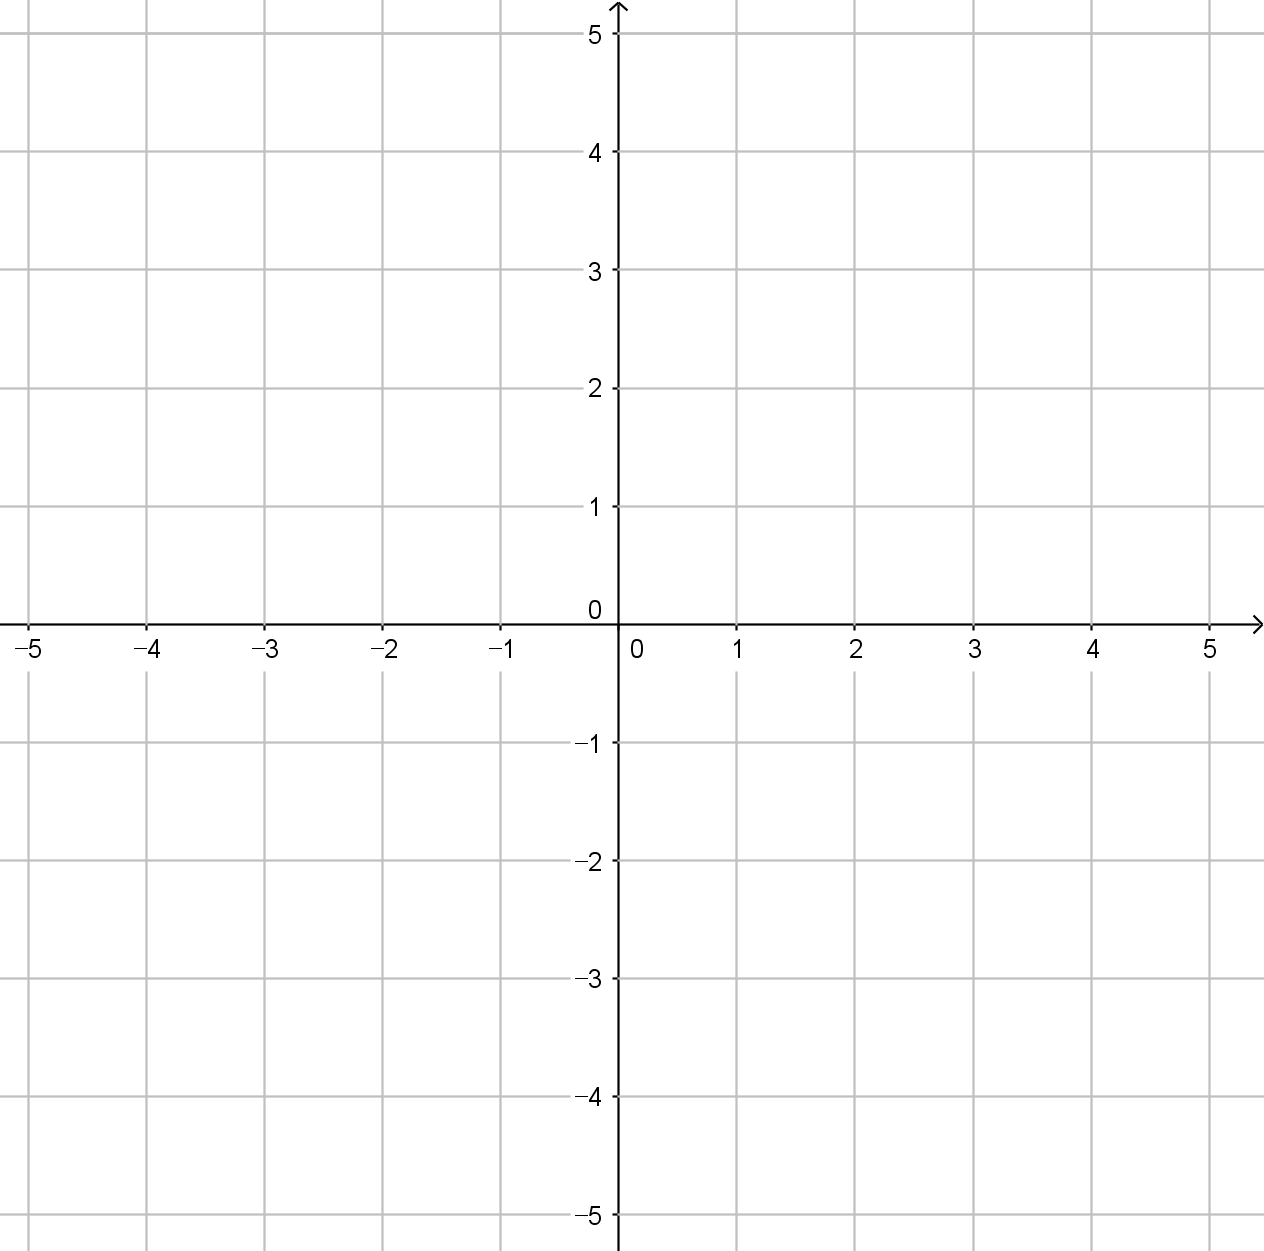
\includegraphics[width=0.9\textwidth]{55}
\end{minipage}
\begin{minipage}{0.45\textwidth}\centering
\(y=-x\)
\par\bigskip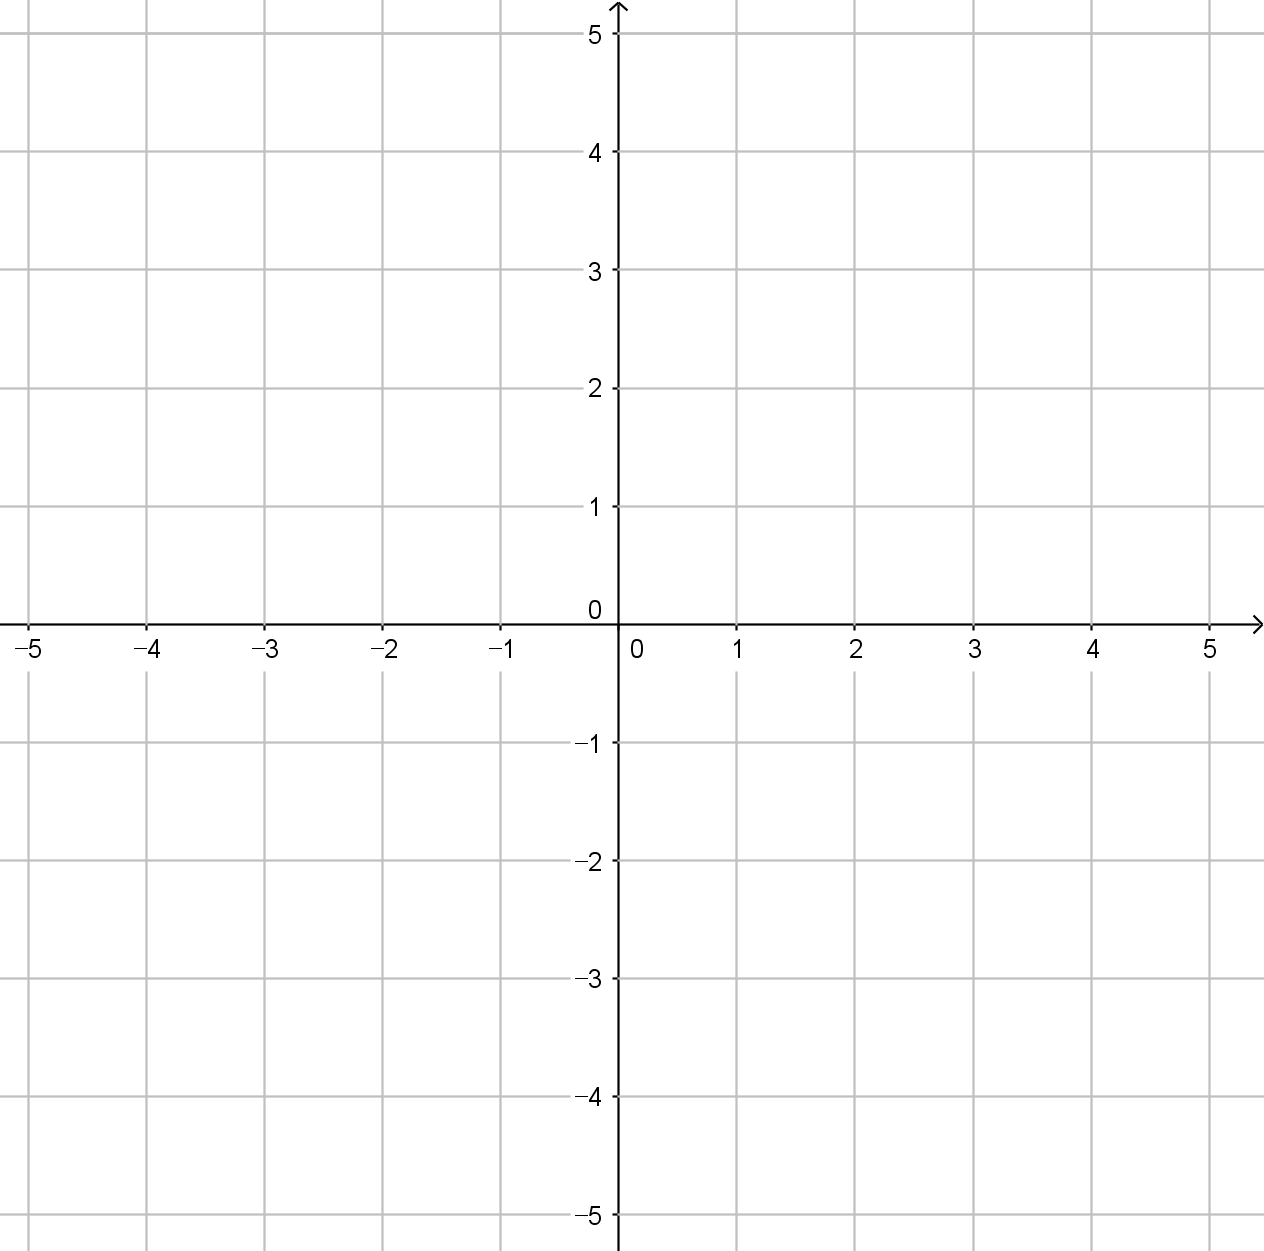
\includegraphics[width=0.9\textwidth]{55}
\end{minipage}\bigskip\bigskip\par
\begin{minipage}{0.45\textwidth}\centering
\(y=2x\)
\par\bigskip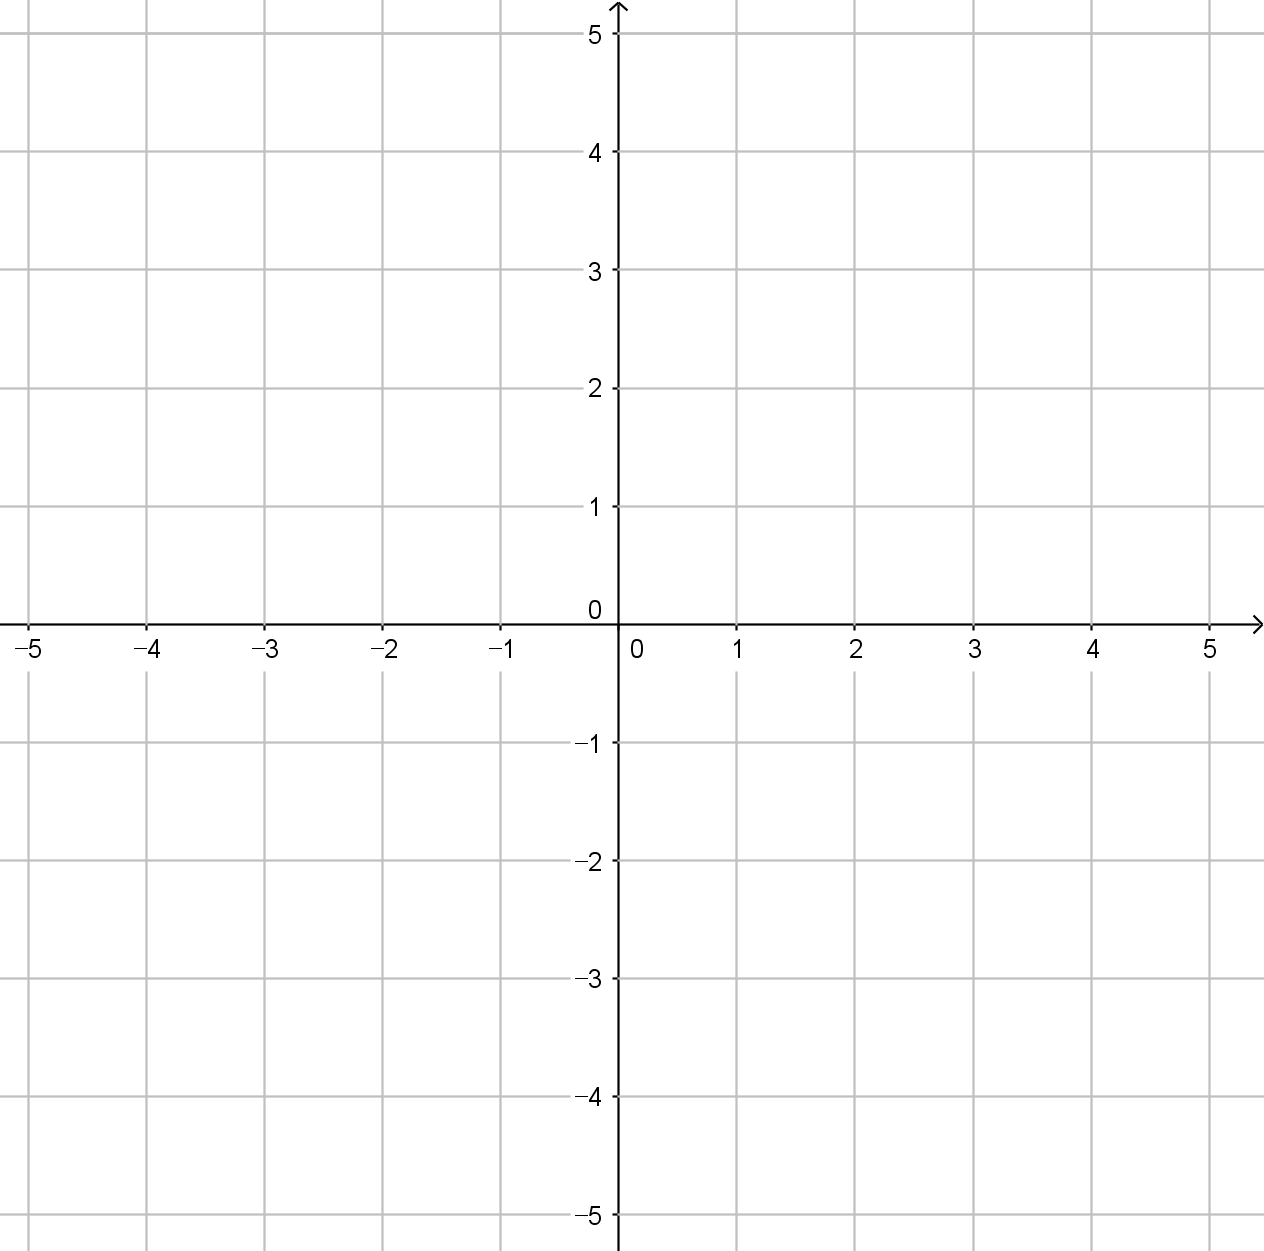
\includegraphics[width=0.9\textwidth]{55}
\end{minipage}
\begin{minipage}{0.45\textwidth}\centering
\(y=-2x\)
\par\bigskip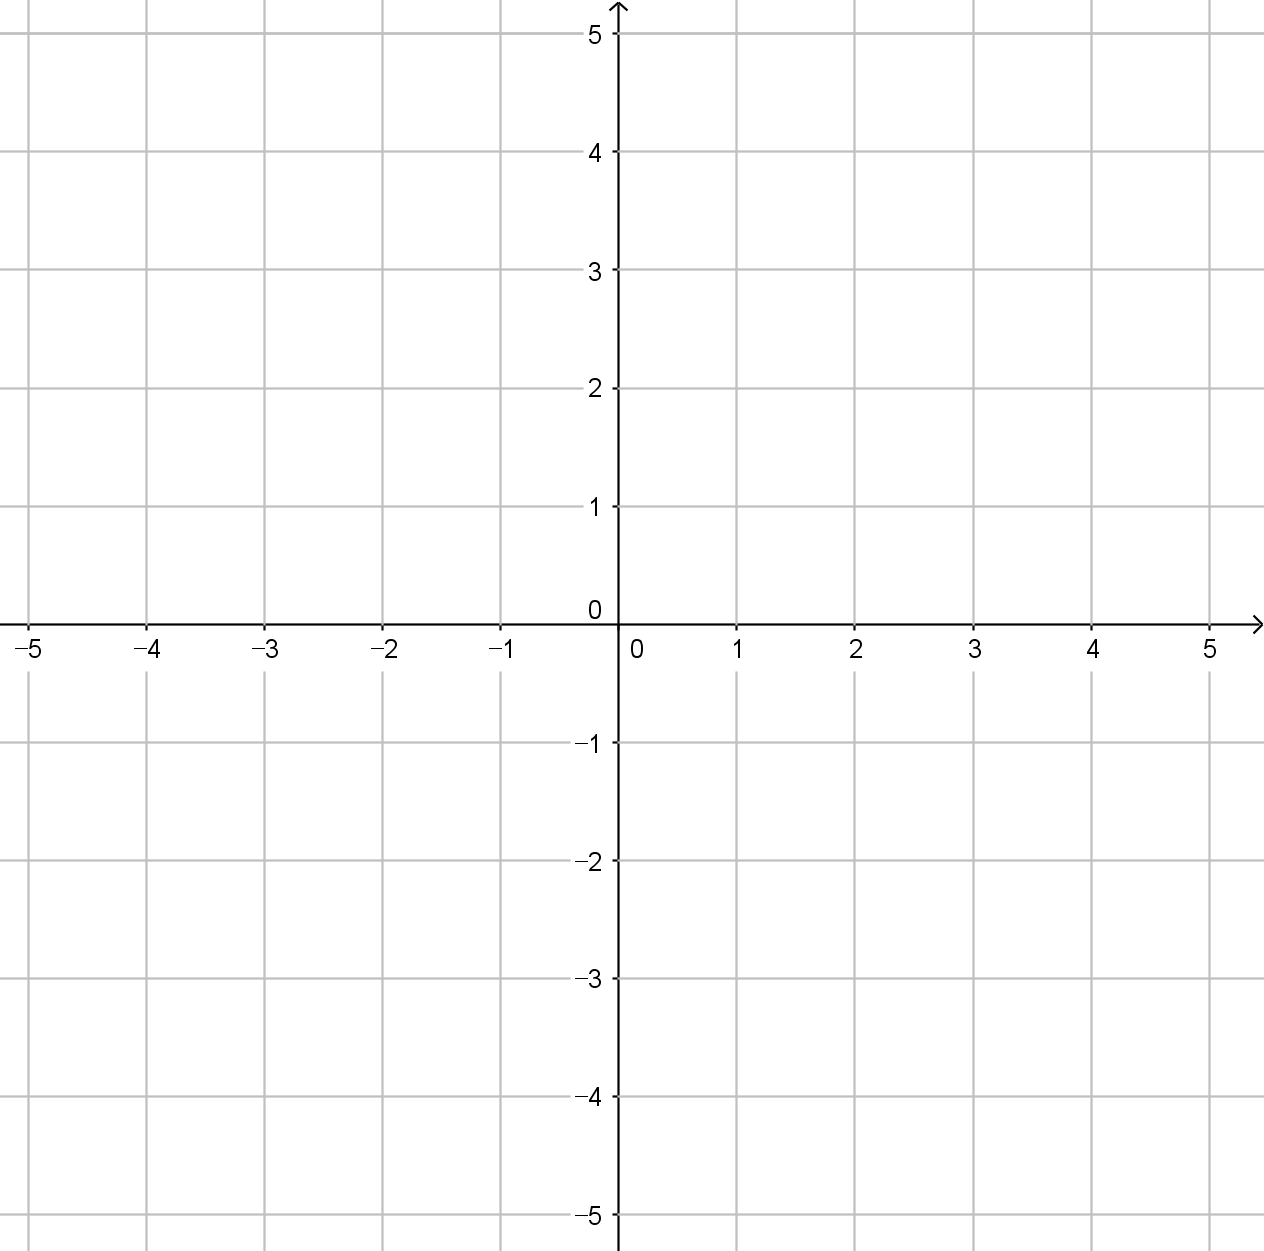
\includegraphics[width=0.9\textwidth]{55}
\end{minipage}\bigskip\bigskip\par

\clearpage
\begin{minipage}{0.45\textwidth}\centering
\(y=x+2\)
\par\bigskip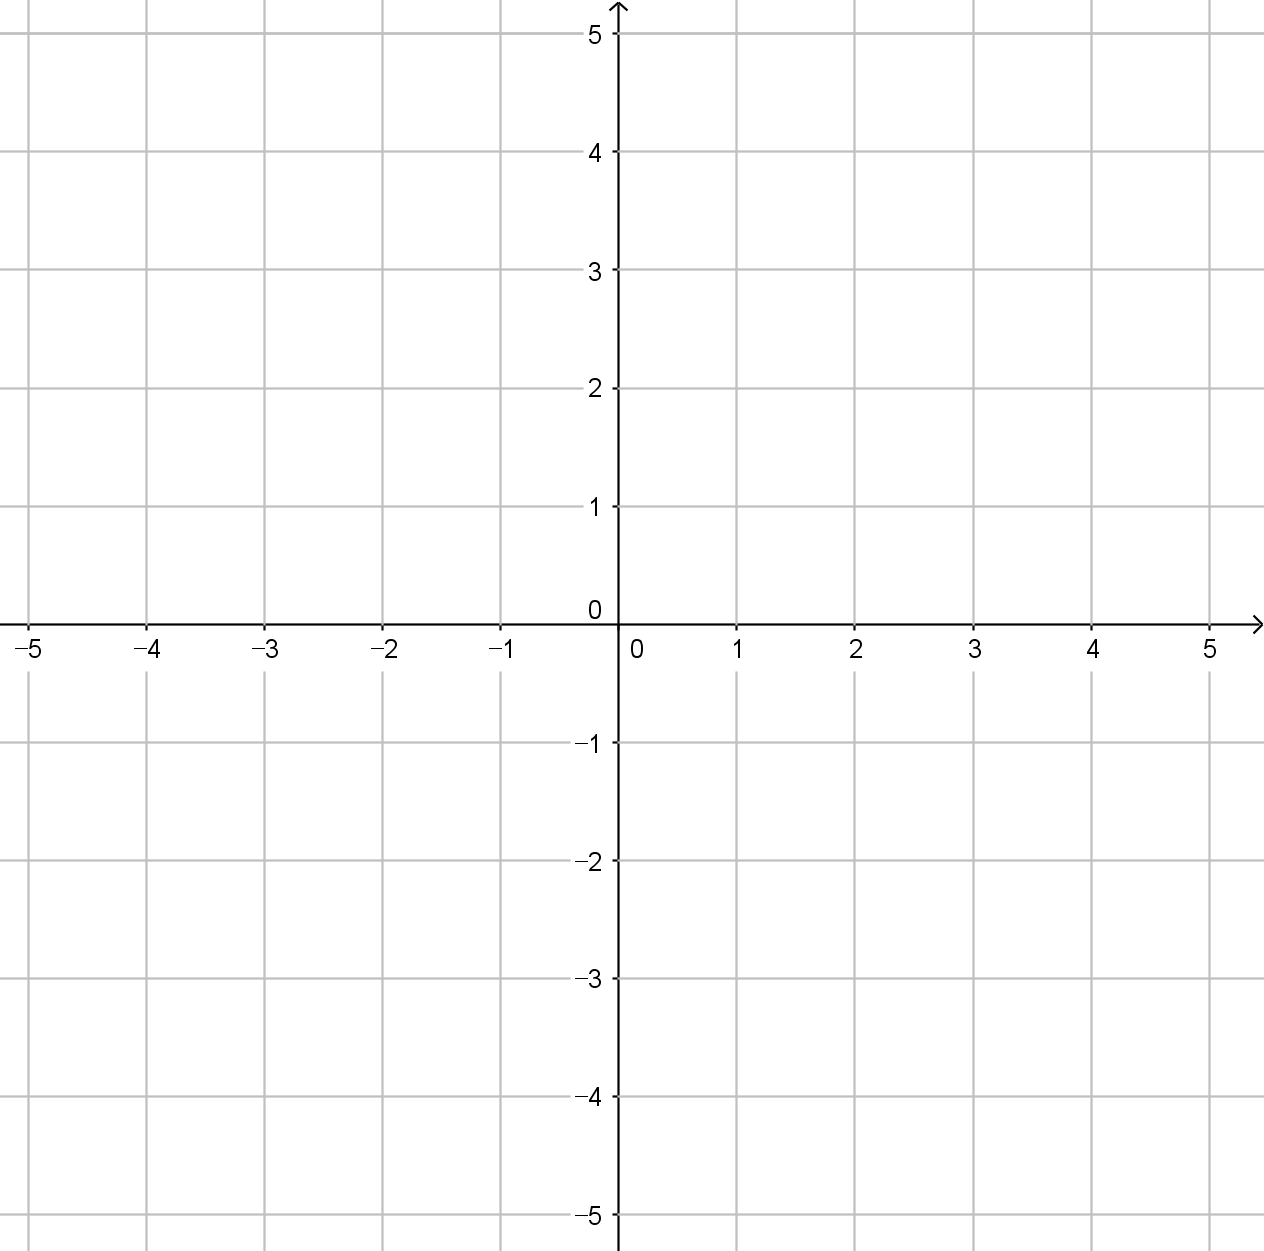
\includegraphics[width=0.9\textwidth]{55}
\end{minipage}
\begin{minipage}{0.45\textwidth}\centering
\(y=x+1\)
\par\bigskip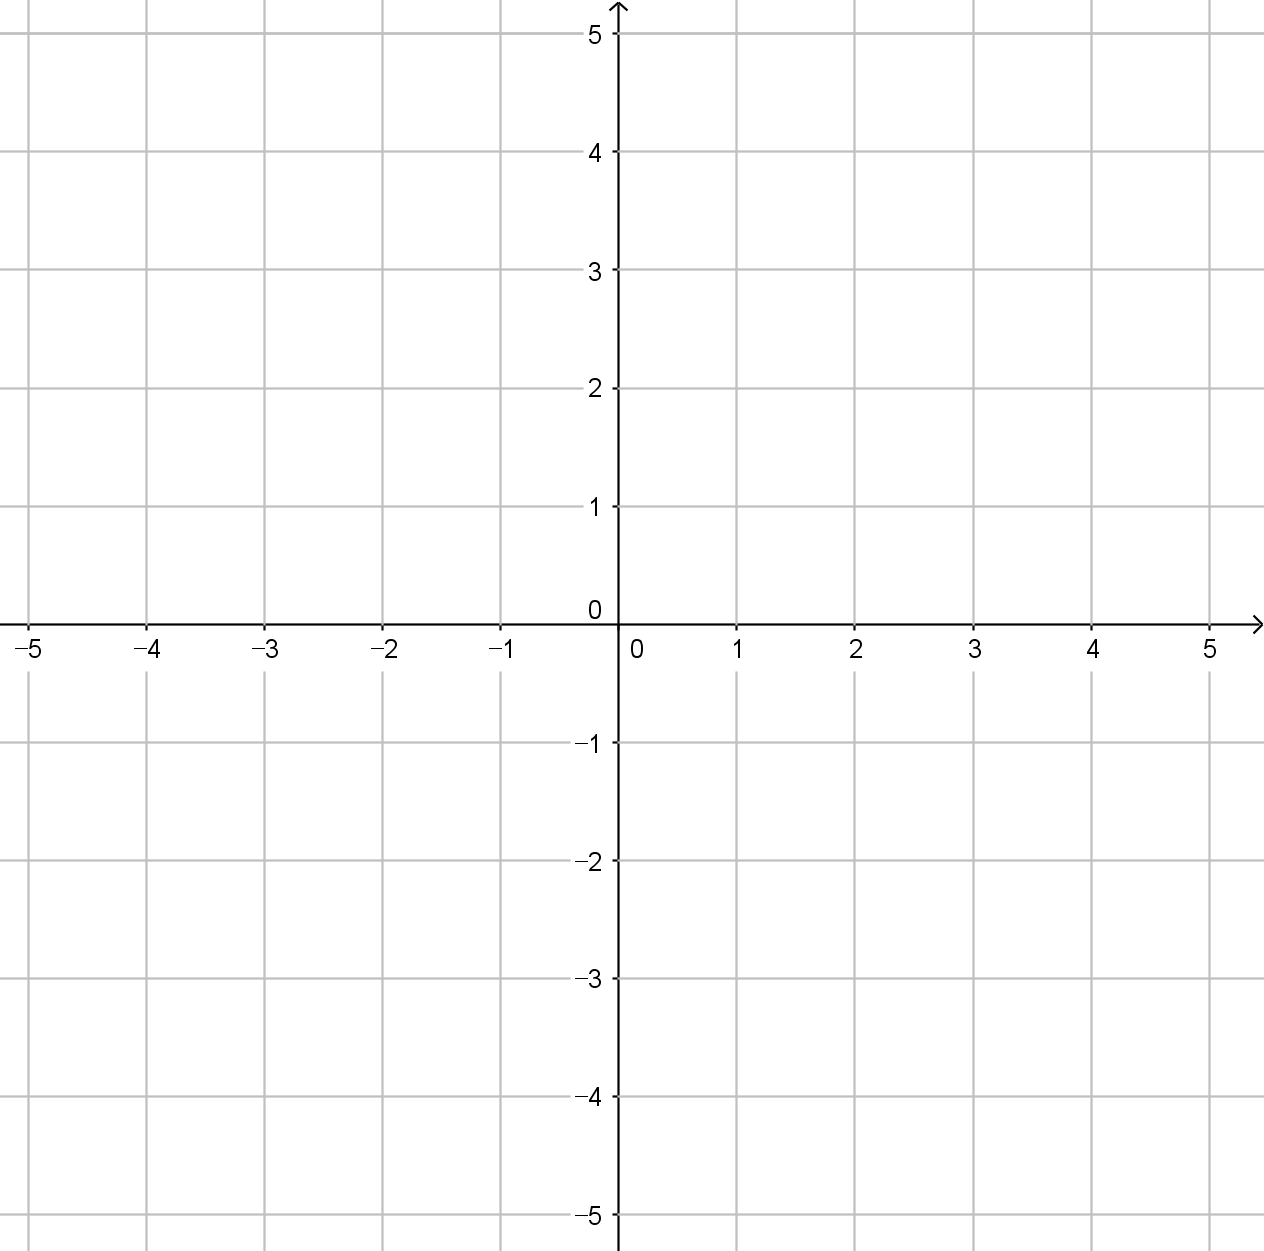
\includegraphics[width=0.9\textwidth]{55}
\end{minipage}\bigskip\bigskip\par
\begin{minipage}{0.45\textwidth}\centering
\(y=x-2\)
\par\bigskip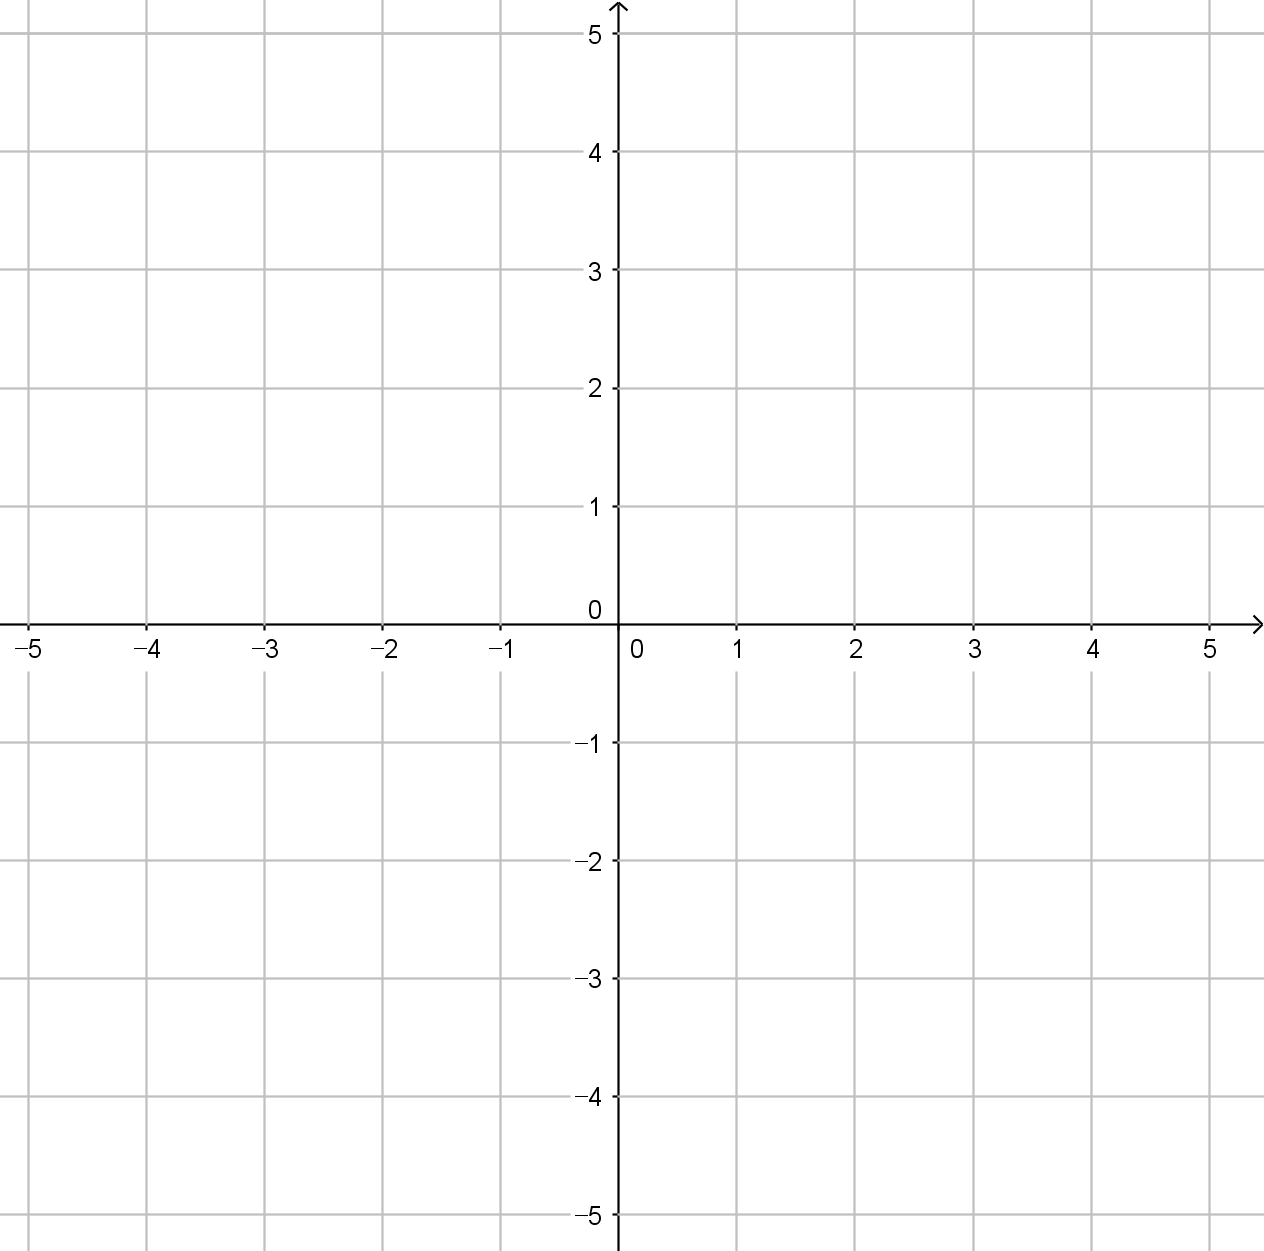
\includegraphics[width=0.9\textwidth]{55}
\end{minipage}
\begin{minipage}{0.45\textwidth}\centering
\(y=2x-2\)
\par\bigskip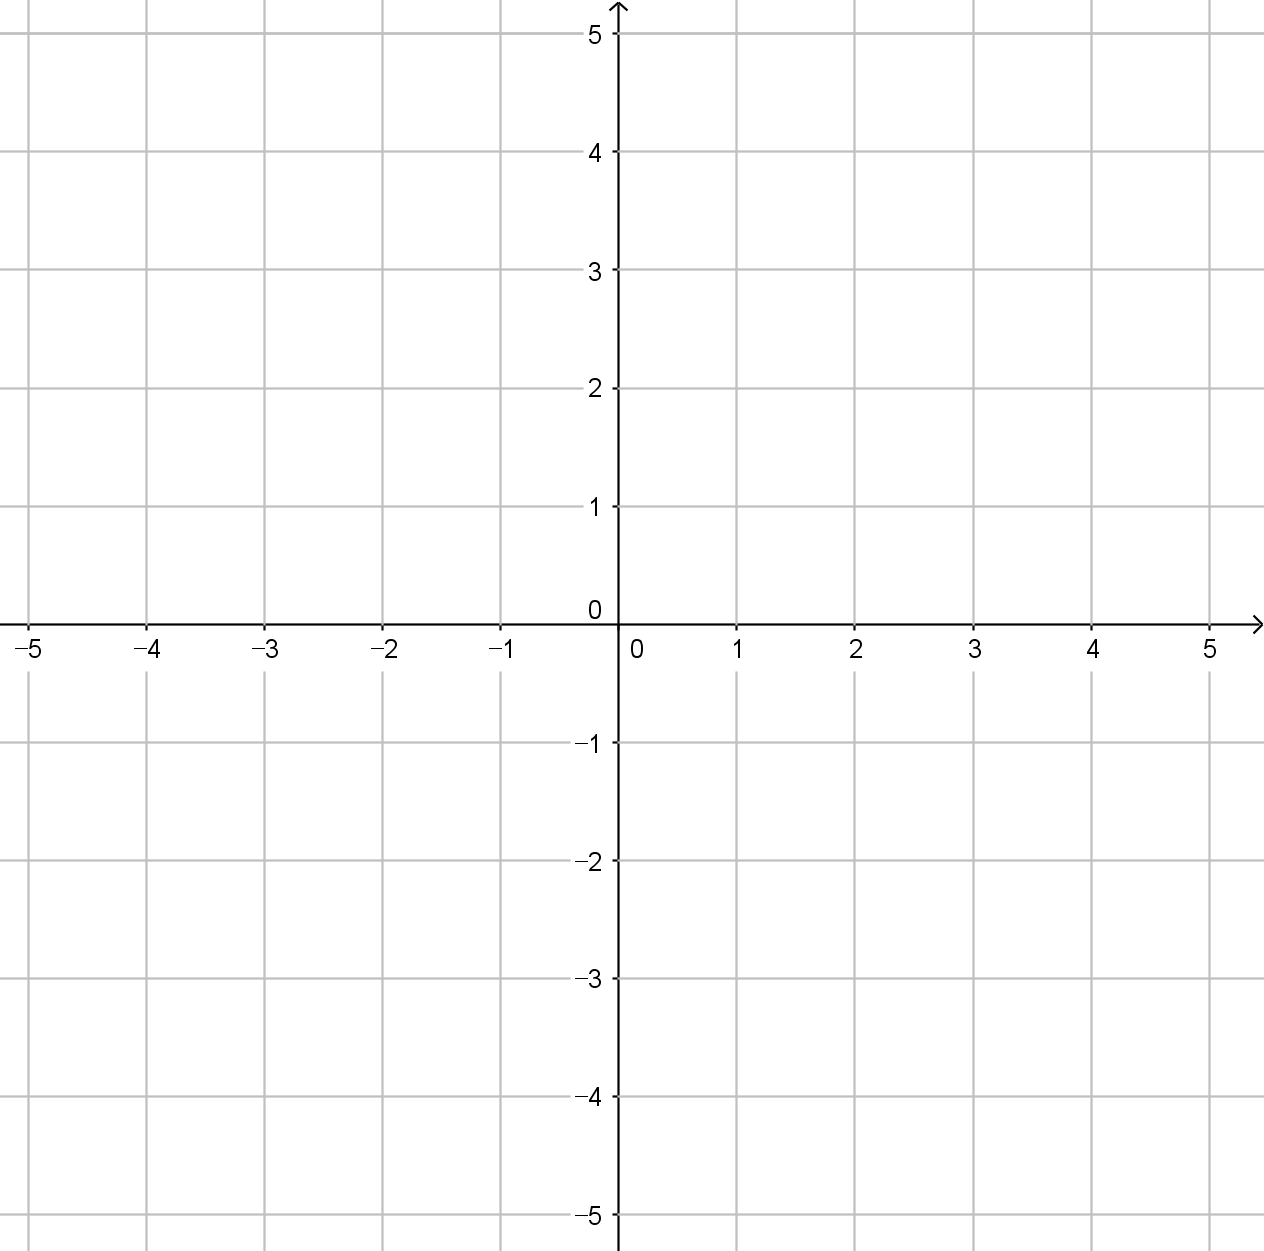
\includegraphics[width=0.9\textwidth]{55}
\end{minipage}\bigskip\bigskip\par
\begin{minipage}{0.45\textwidth}\centering
\(y=2x+1\)
\par\bigskip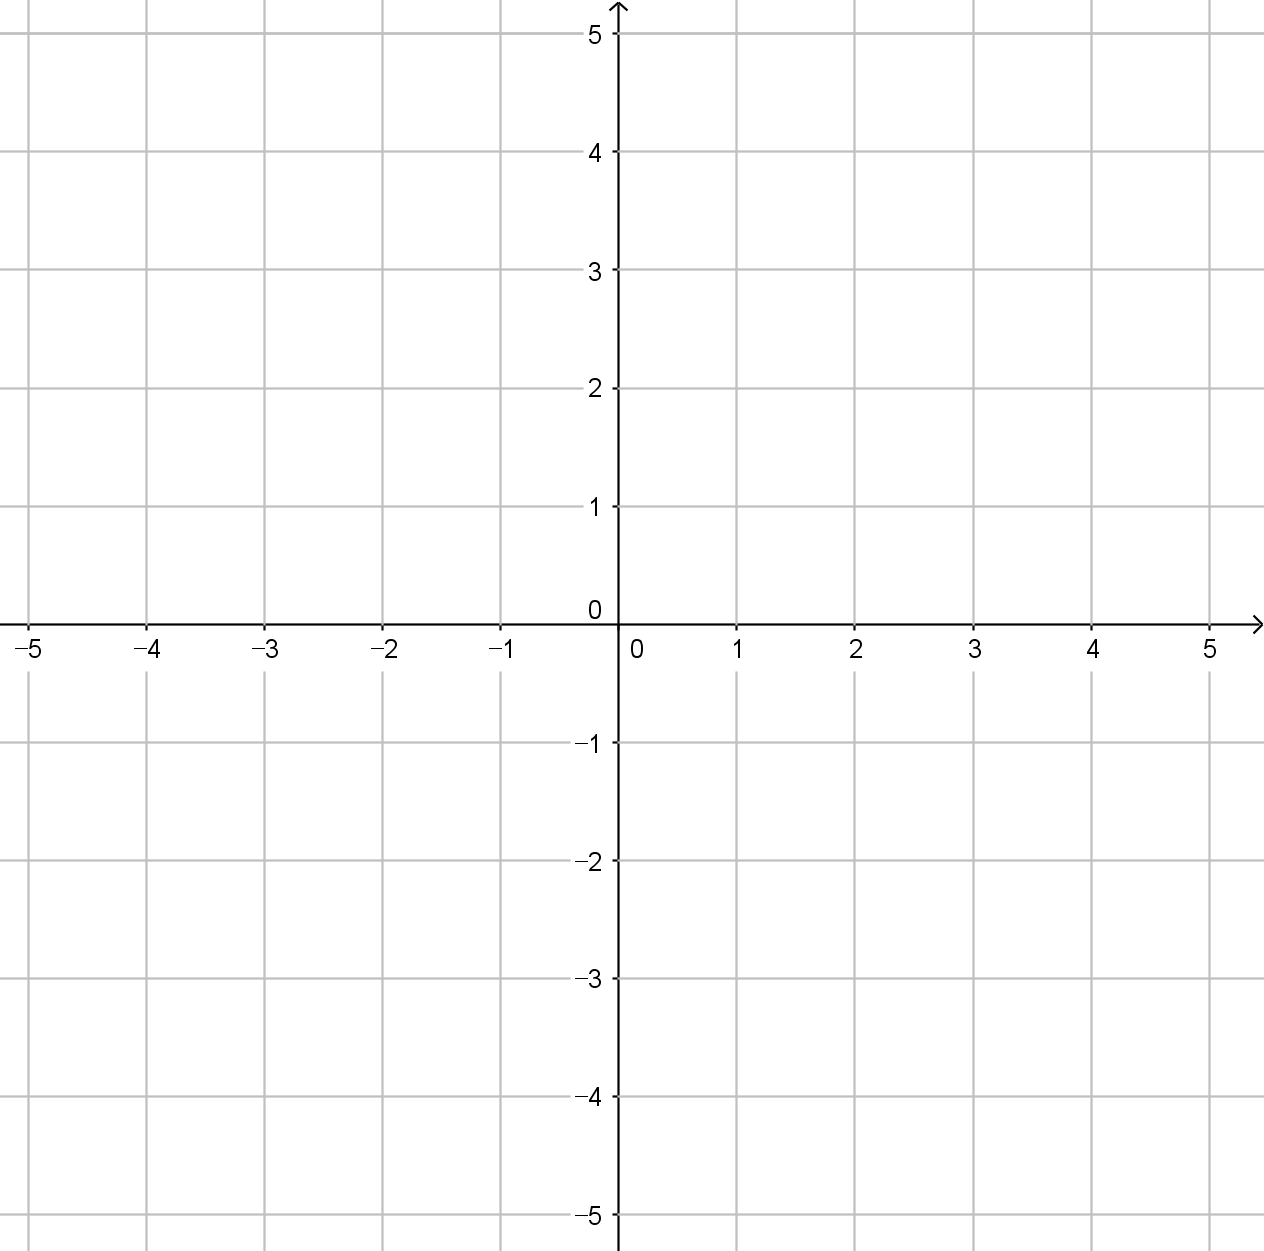
\includegraphics[width=0.9\textwidth]{55}
\end{minipage}
\begin{minipage}{0.45\textwidth}\centering
\(y=2x\)
\par\bigskip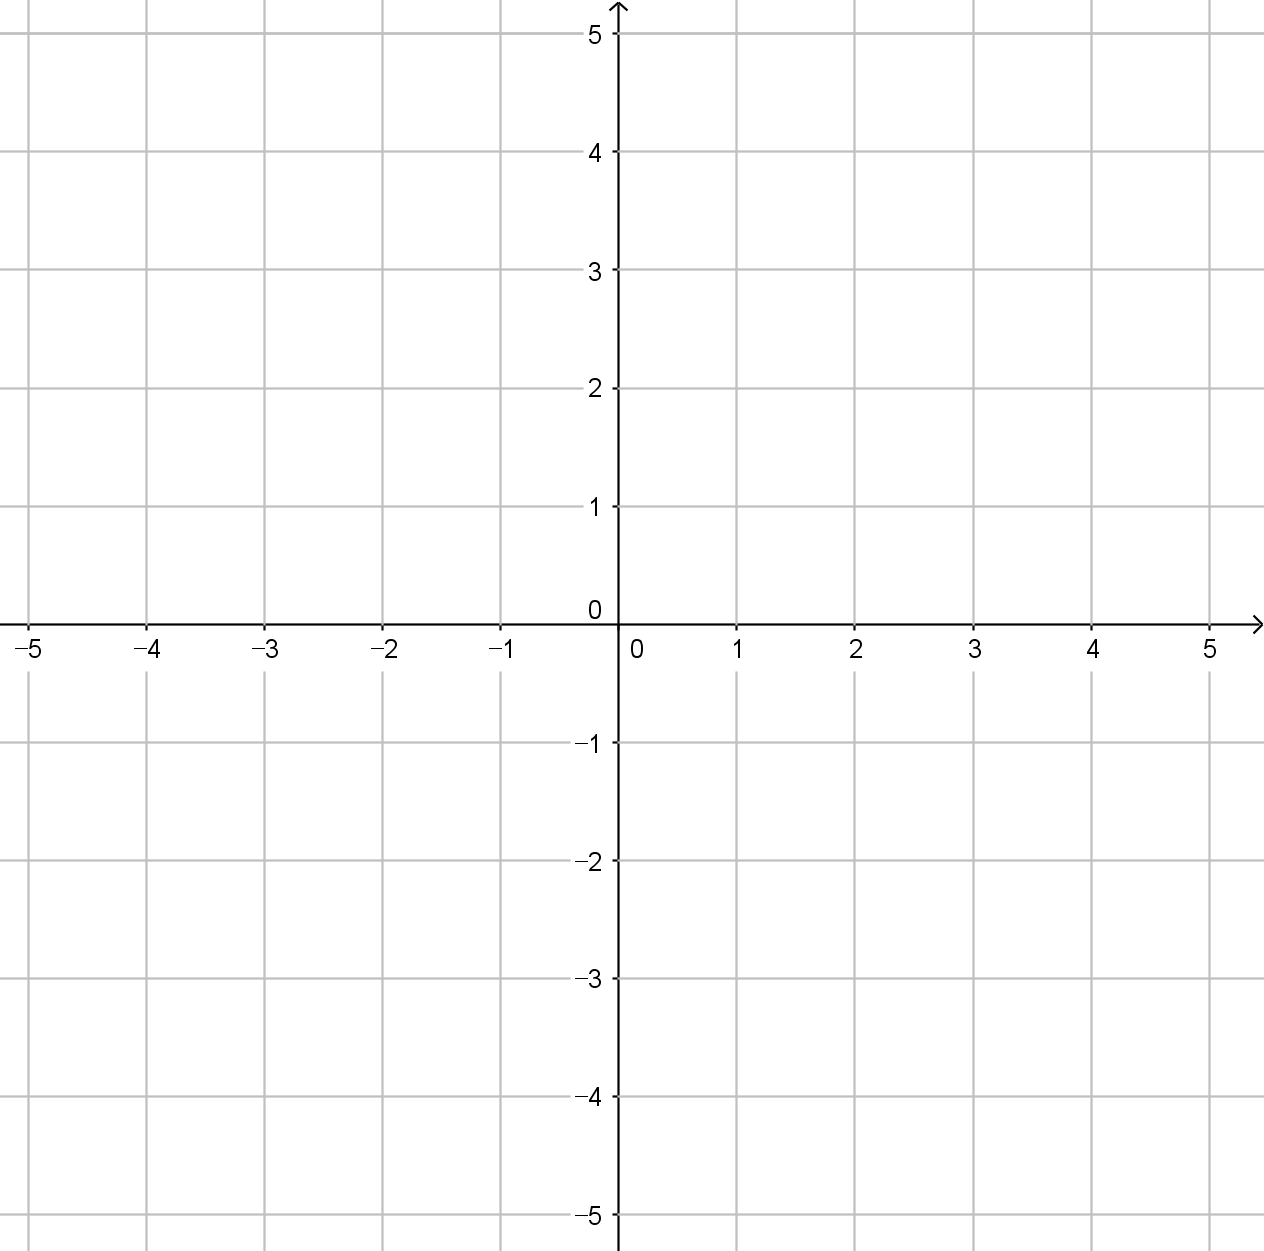
\includegraphics[width=0.9\textwidth]{55}
\end{minipage}\bigskip\bigskip\par

\clearpage
\begin{minipage}{0.45\textwidth}\centering
\(y=3x-3\)
\par\bigskip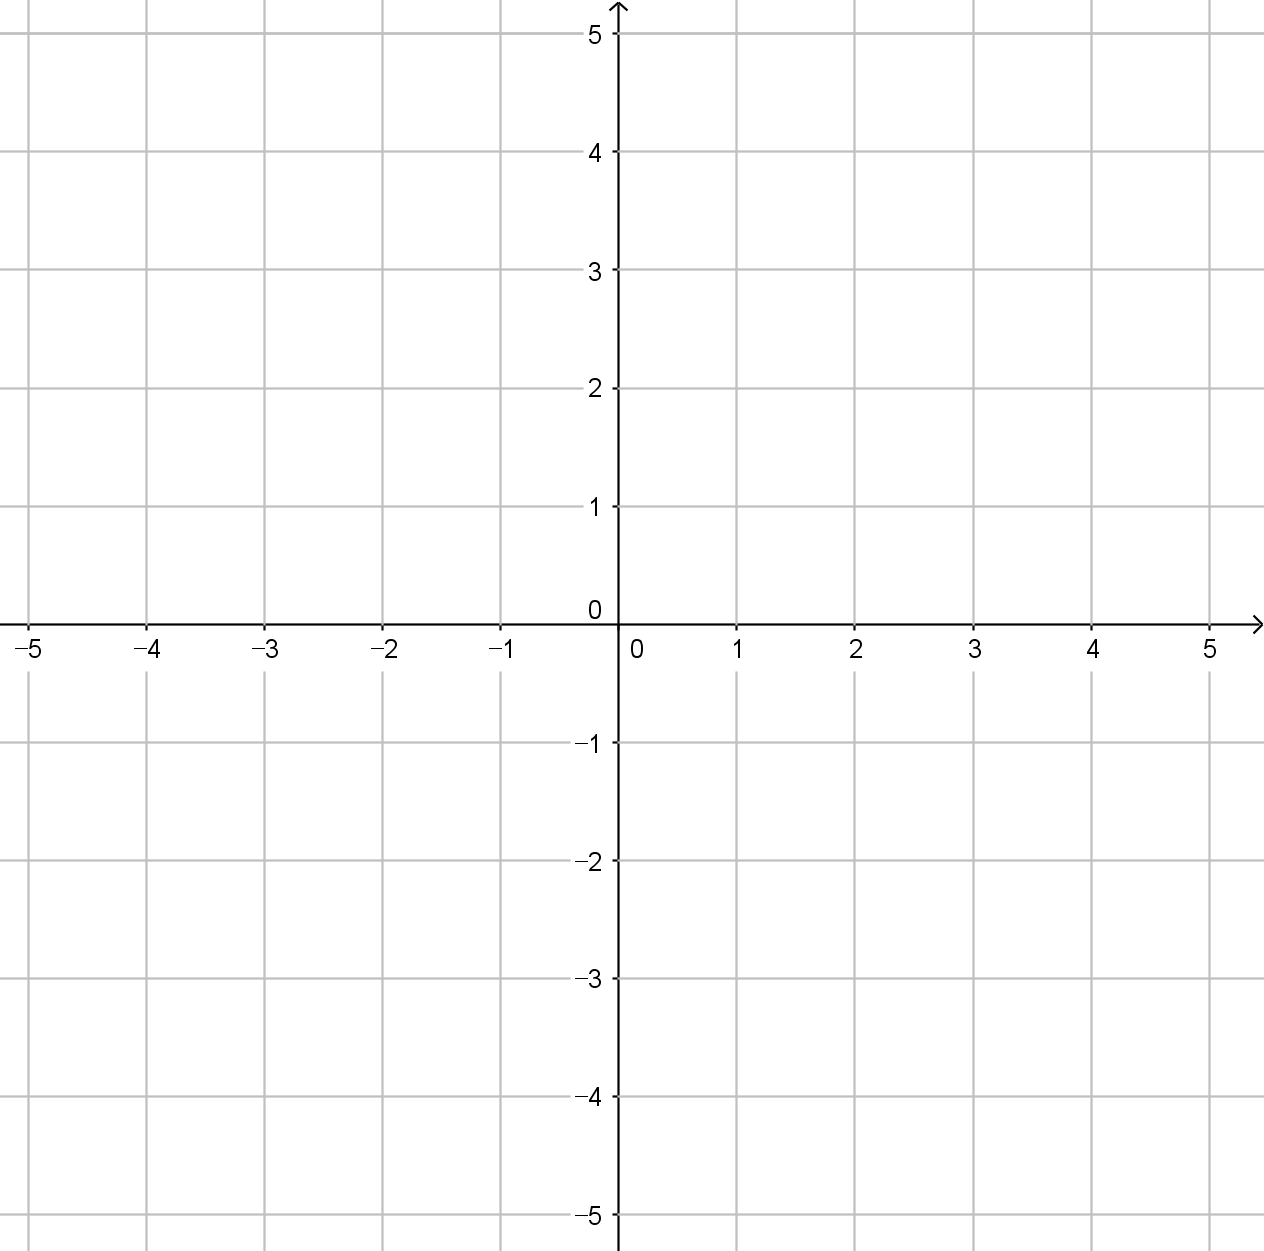
\includegraphics[width=0.9\textwidth]{55}
\end{minipage}
\begin{minipage}{0.45\textwidth}\centering
\(y=3x+2\)
\par\bigskip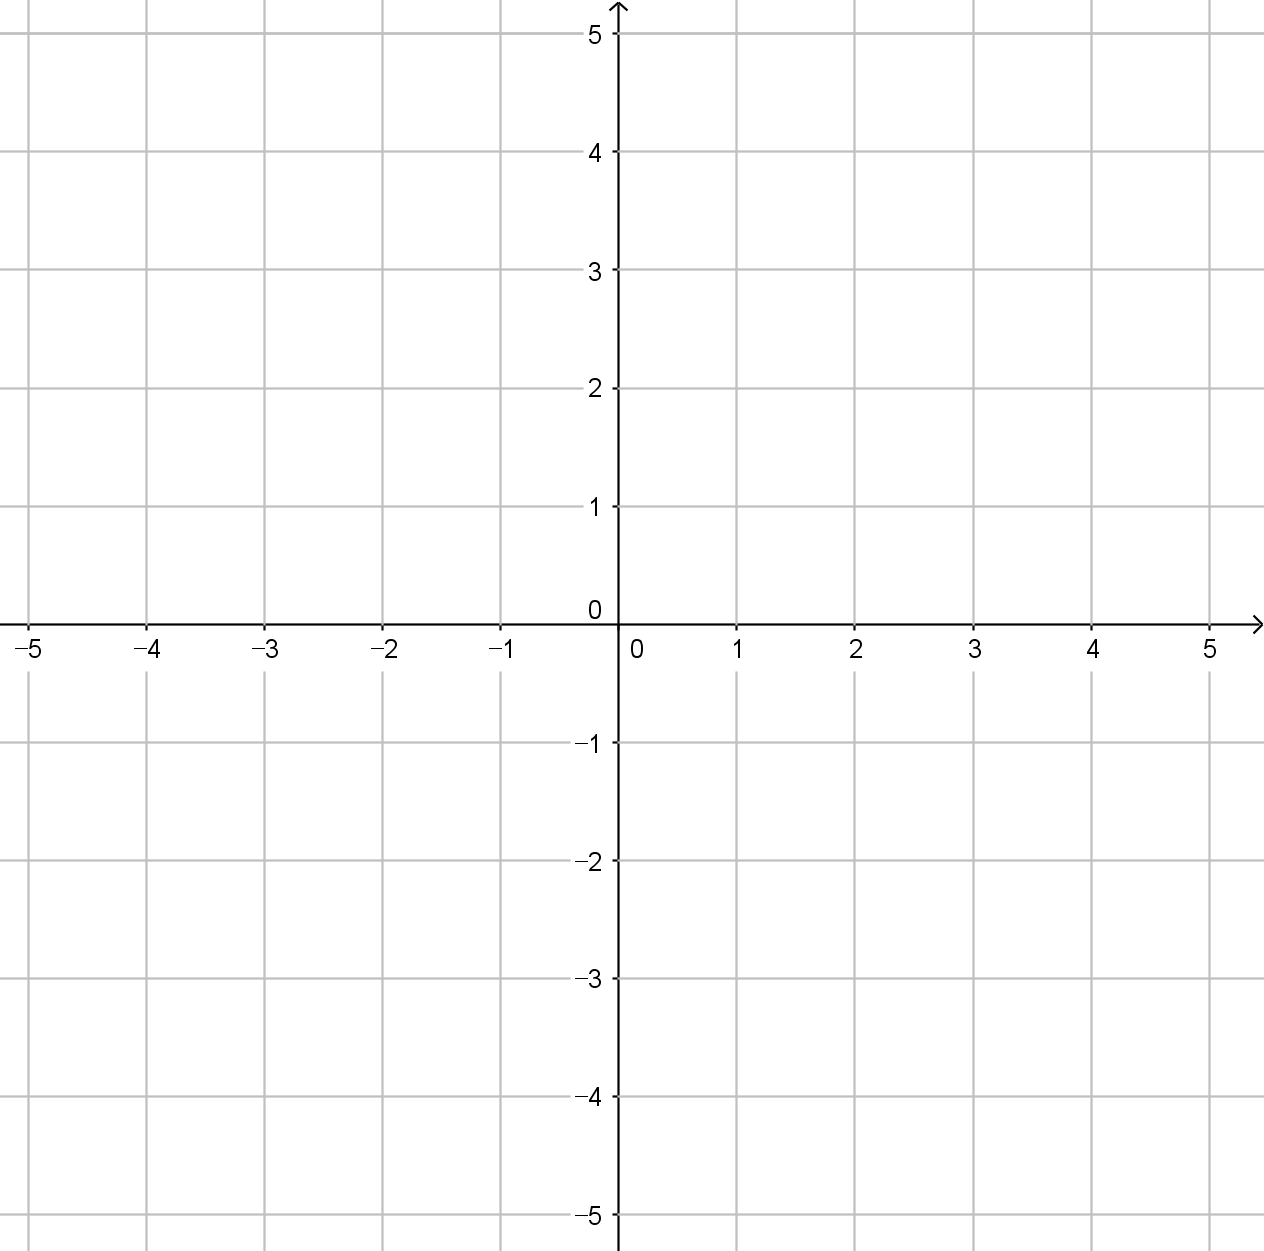
\includegraphics[width=0.9\textwidth]{55}
\end{minipage}\bigskip\bigskip\par
\begin{minipage}{0.45\textwidth}\centering
\(y=-x+2\)
\par\bigskip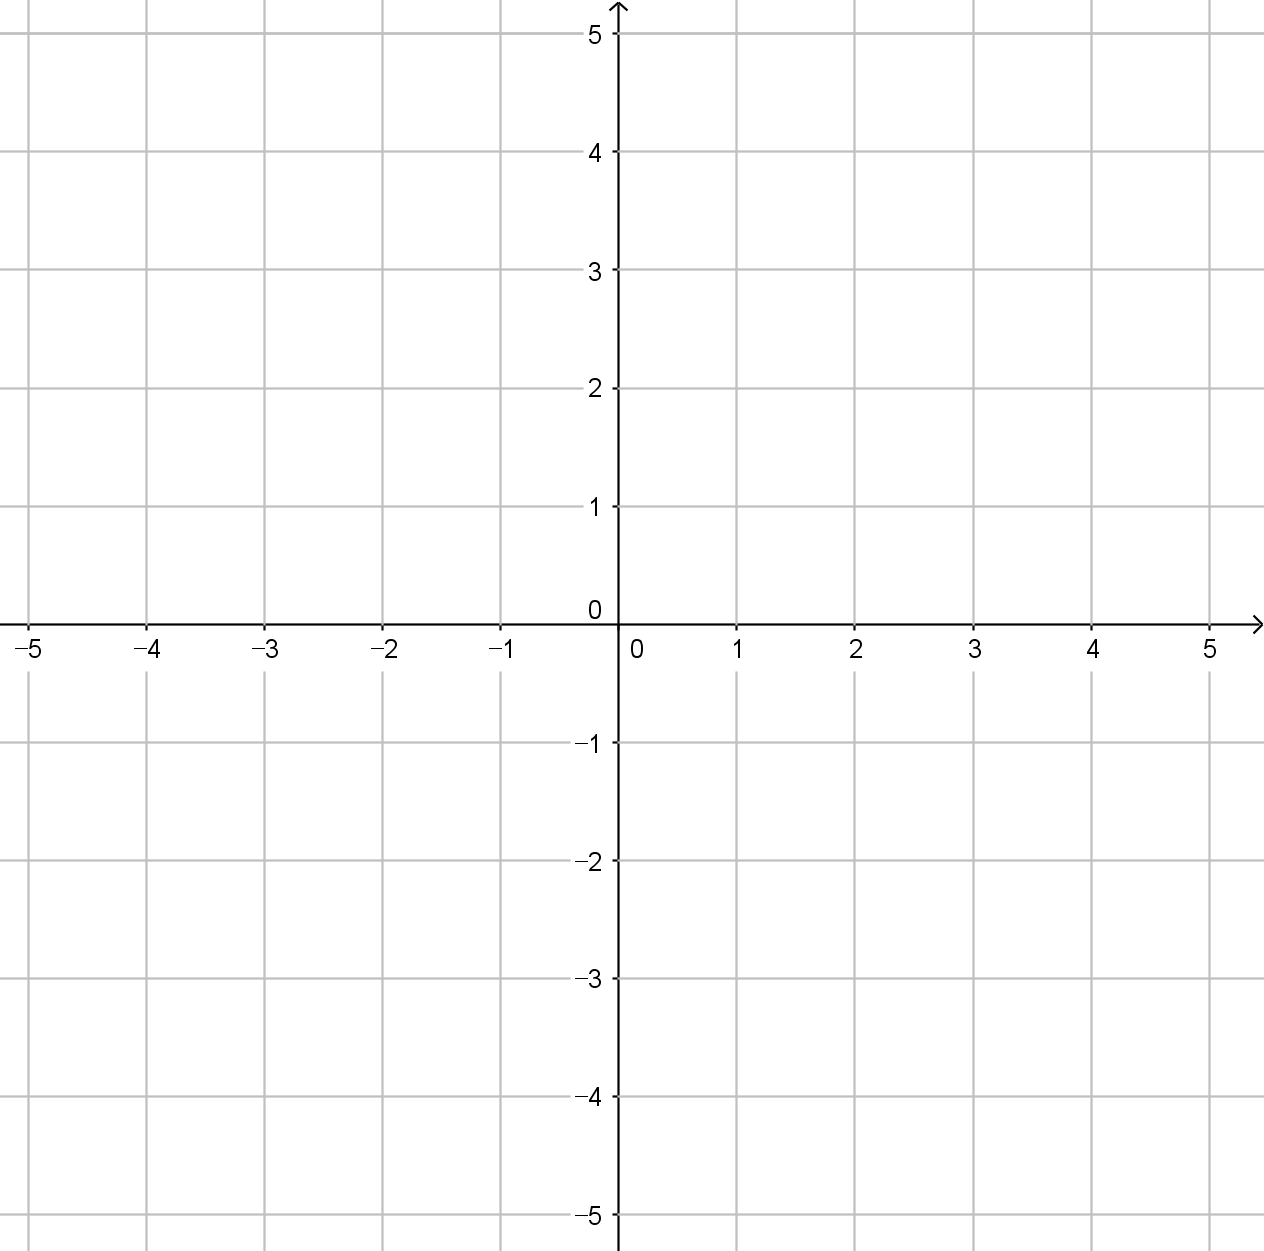
\includegraphics[width=0.9\textwidth]{55}
\end{minipage}
\begin{minipage}{0.45\textwidth}\centering
\(y=-x-3\)
\par\bigskip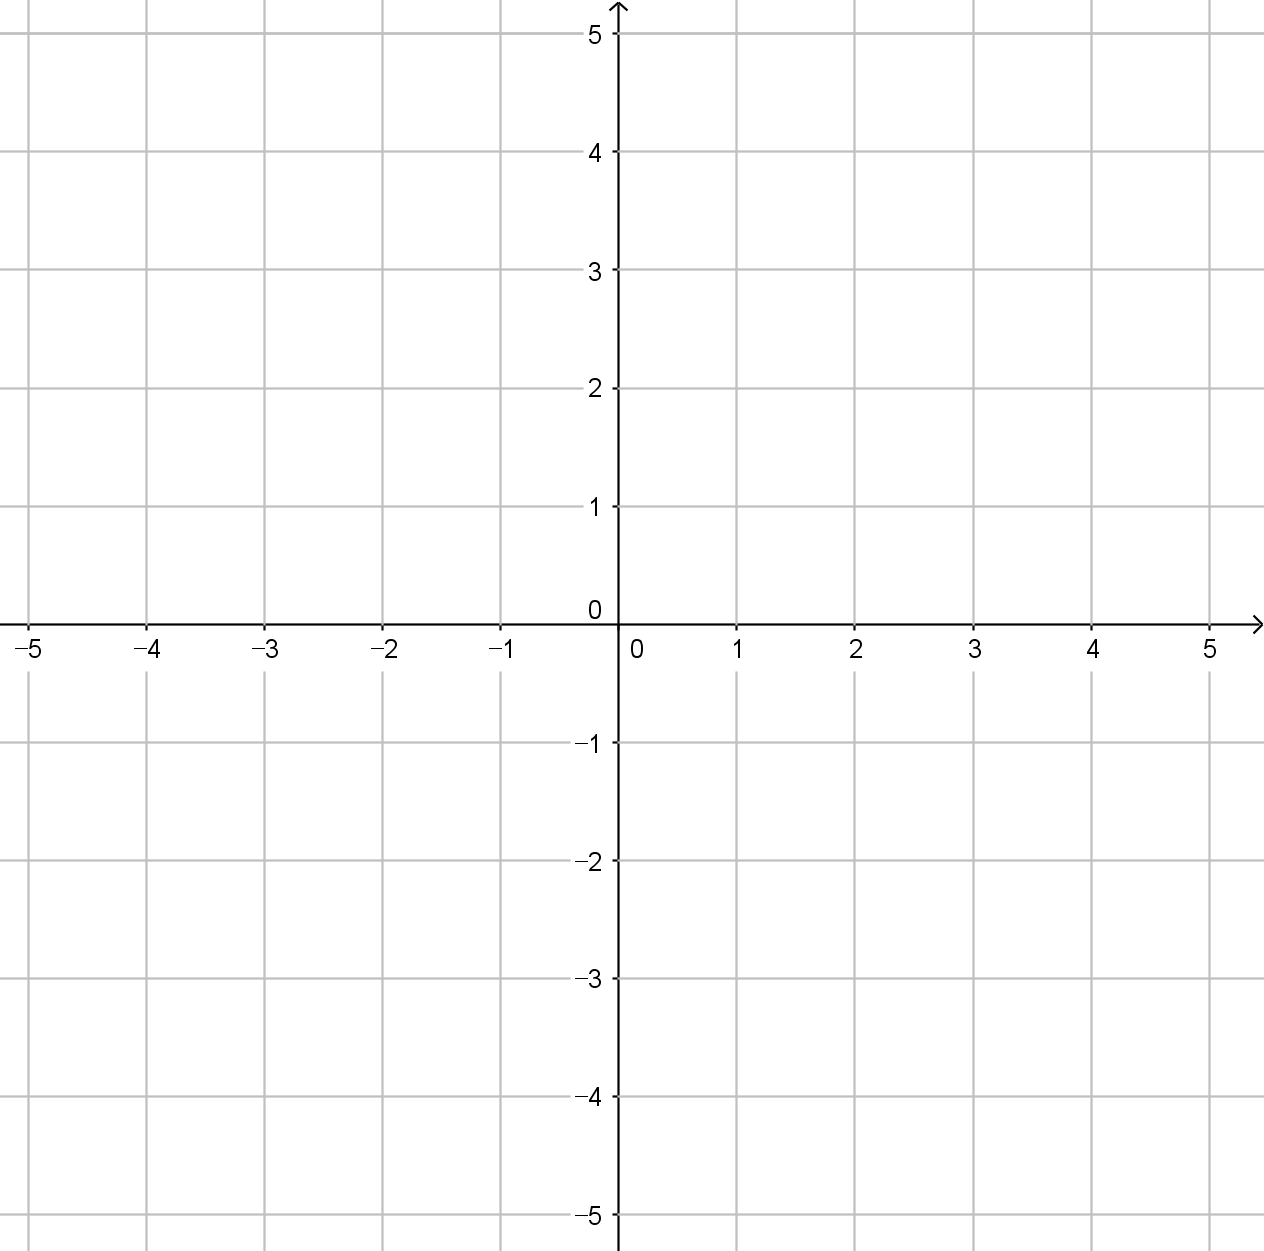
\includegraphics[width=0.9\textwidth]{55}
\end{minipage}\bigskip\bigskip\par
\begin{minipage}{0.45\textwidth}\centering
\(y=-2x+5\)
\par\bigskip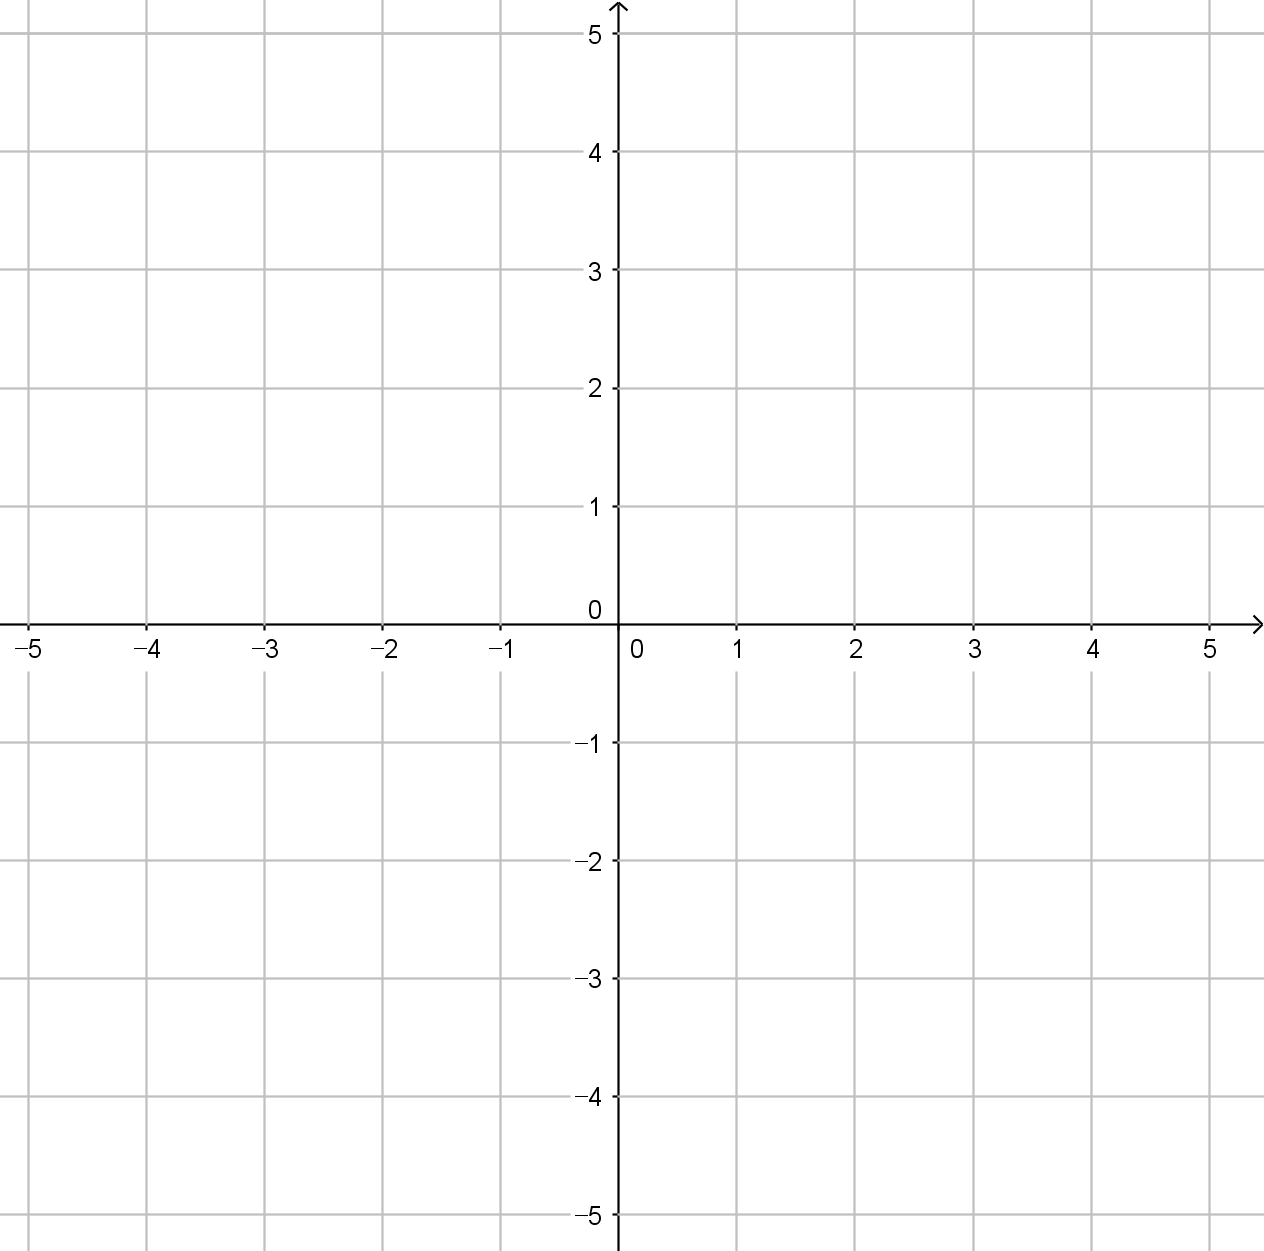
\includegraphics[width=0.9\textwidth]{55}
\end{minipage}
\begin{minipage}{0.45\textwidth}\centering
\(y=-3x+3\)
\par\bigskip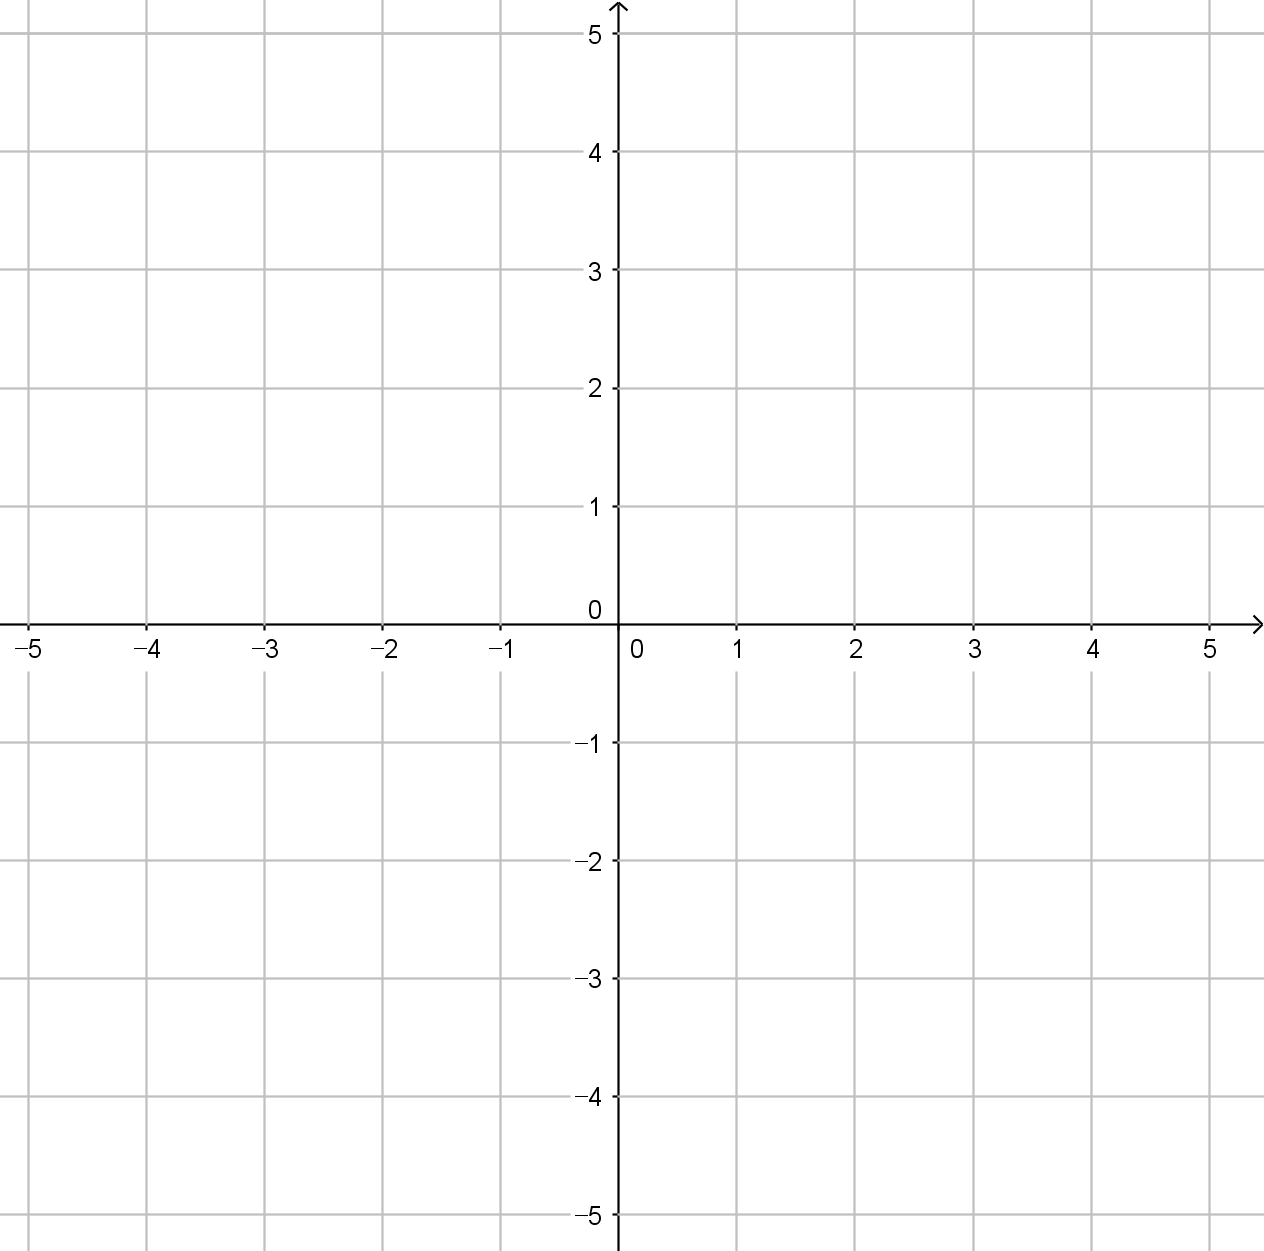
\includegraphics[width=0.9\textwidth]{55}
\end{minipage}\bigskip\bigskip\par


\clearpage
\begin{minipage}{0.45\textwidth}\centering
\(y=\frac12x-2\)
\par\bigskip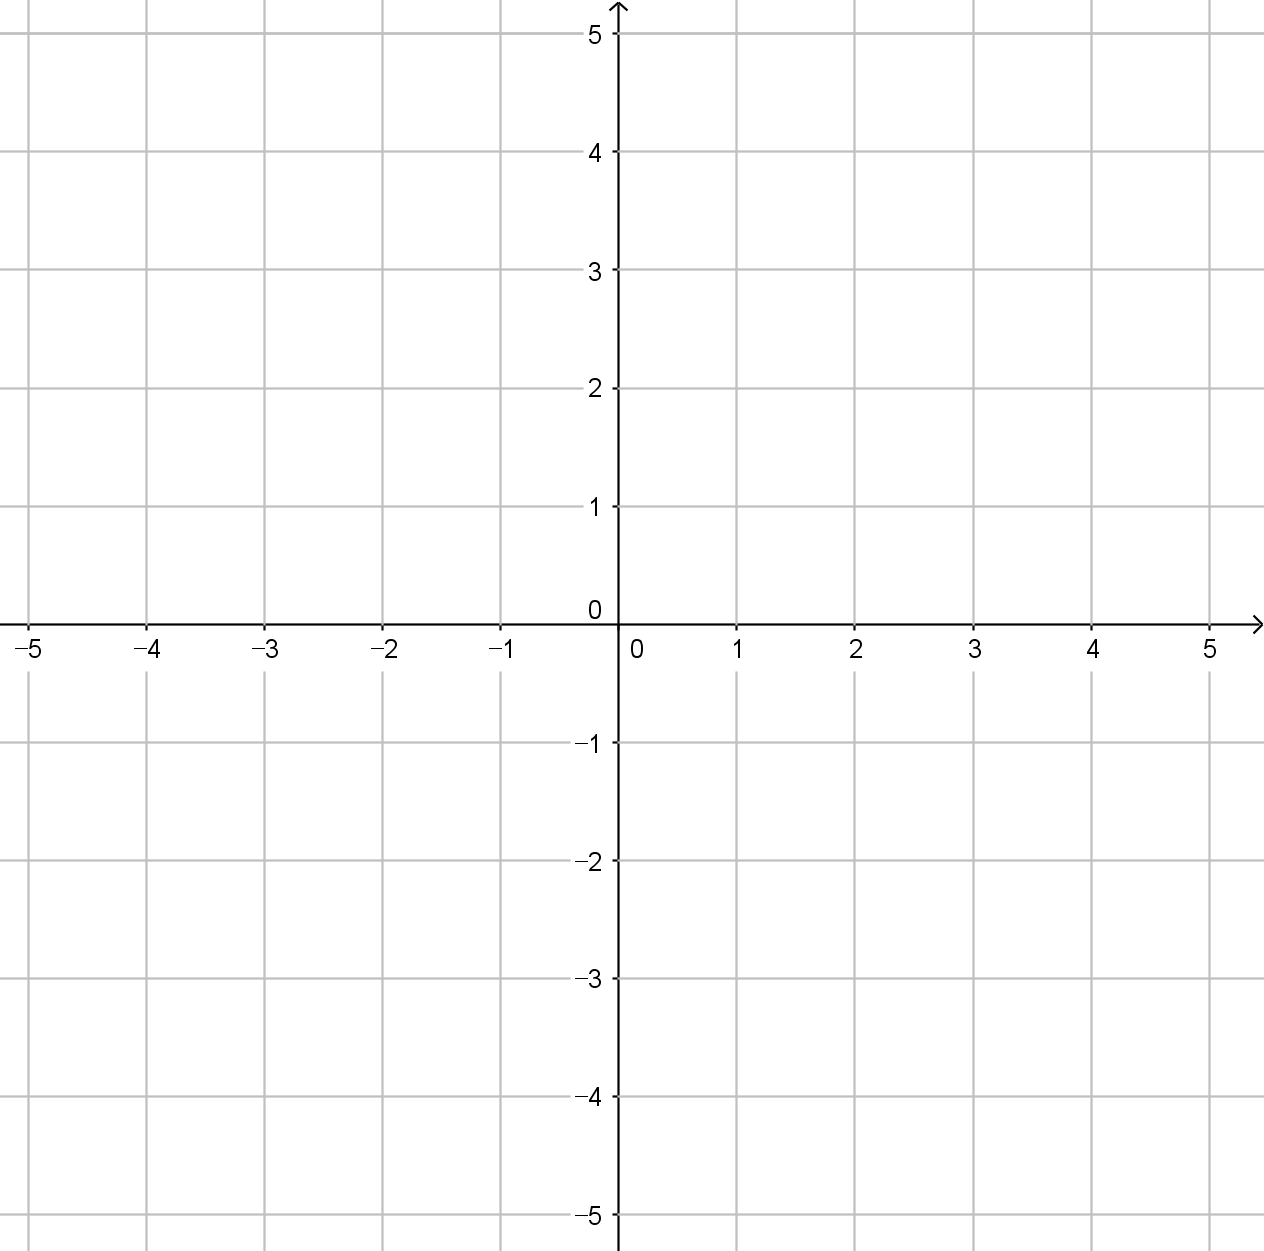
\includegraphics[width=0.9\textwidth]{55}
\end{minipage}
\begin{minipage}{0.45\textwidth}\centering
\(y=\frac12x+1\)
\par\bigskip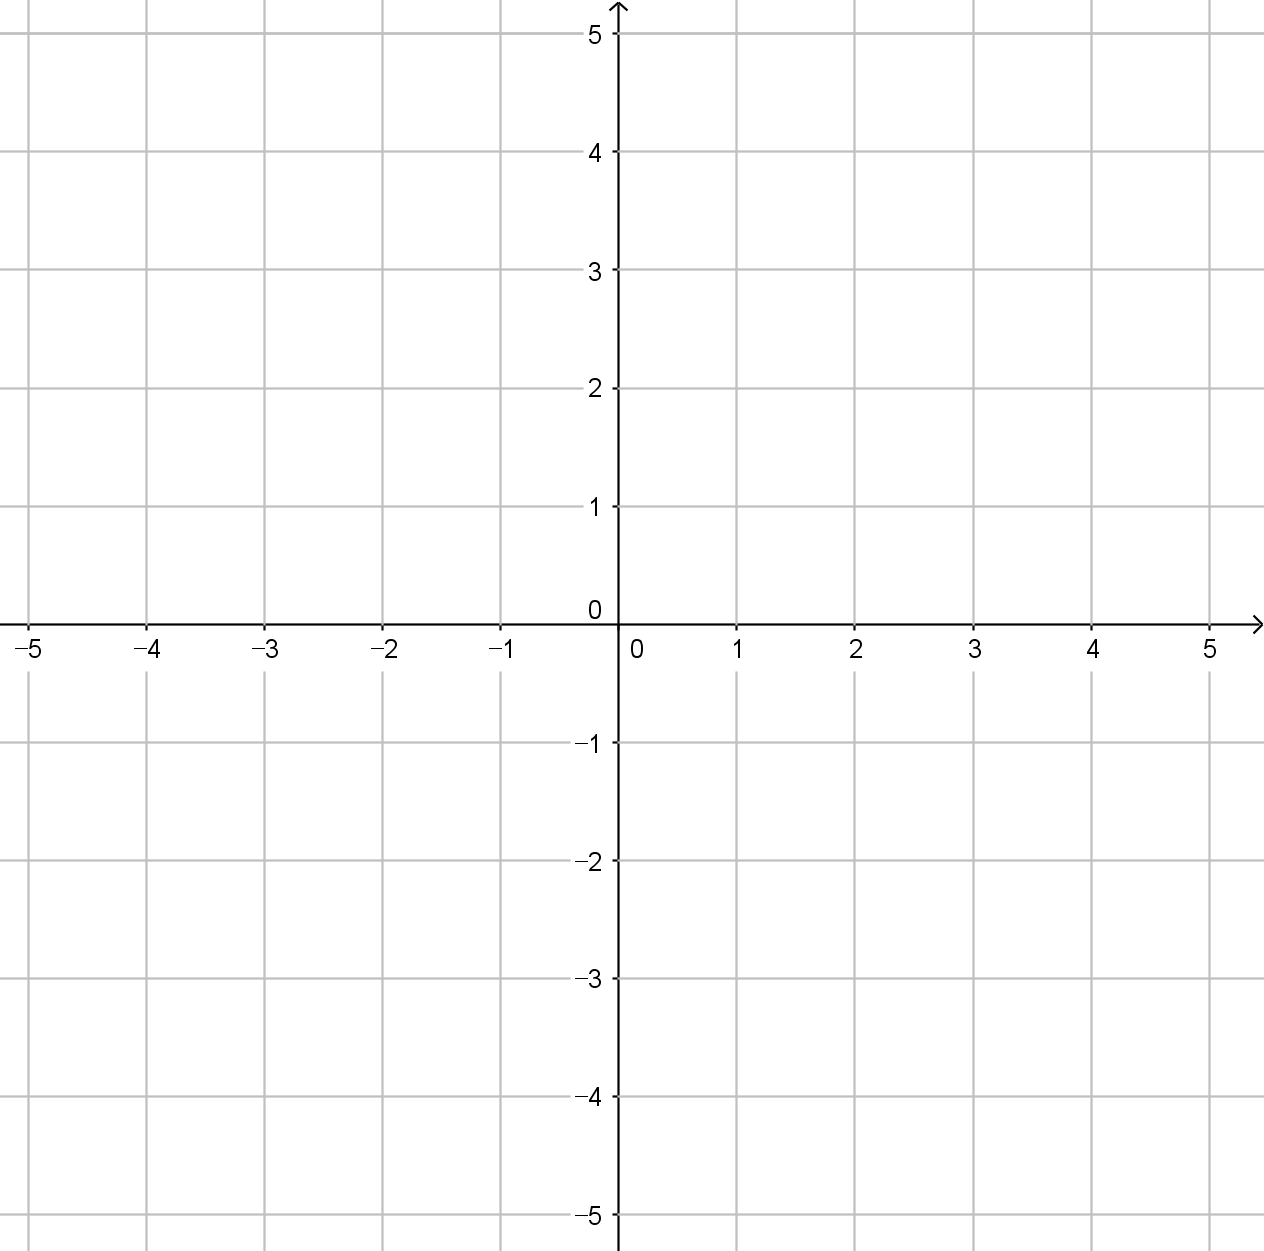
\includegraphics[width=0.9\textwidth]{55}
\end{minipage}\bigskip\bigskip\par
\begin{minipage}{0.45\textwidth}\centering
\(y=-\frac12x\)
\par\bigskip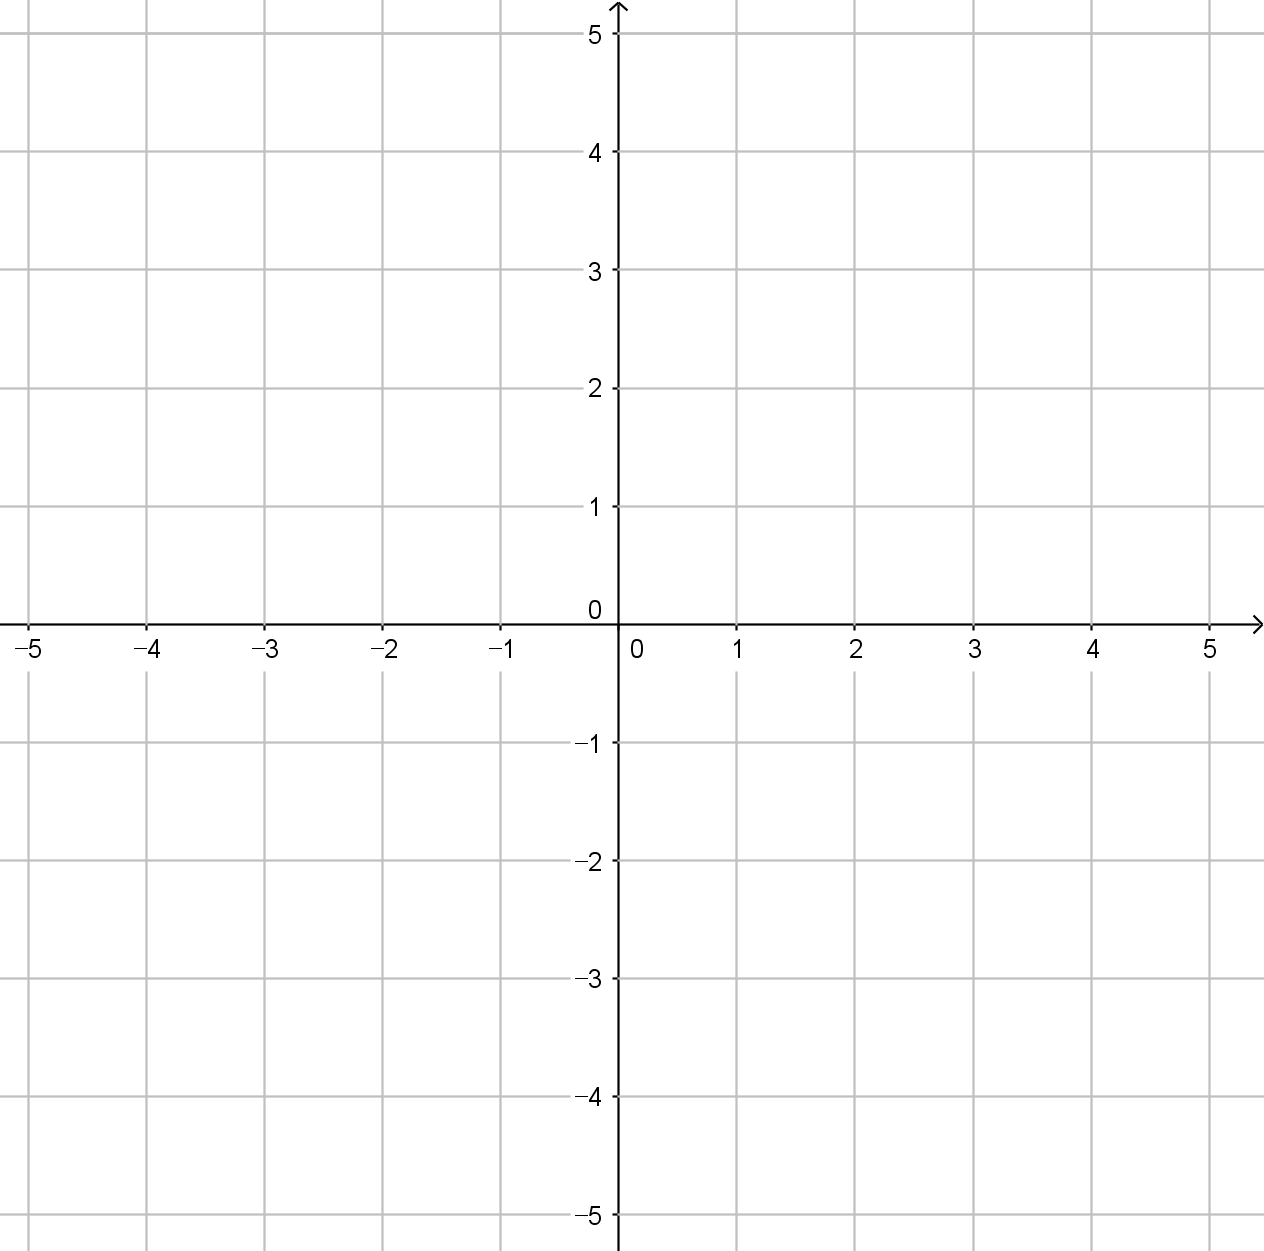
\includegraphics[width=0.9\textwidth]{55}
\end{minipage}
\begin{minipage}{0.45\textwidth}\centering
\(y=\frac13x-1\)
\par\bigskip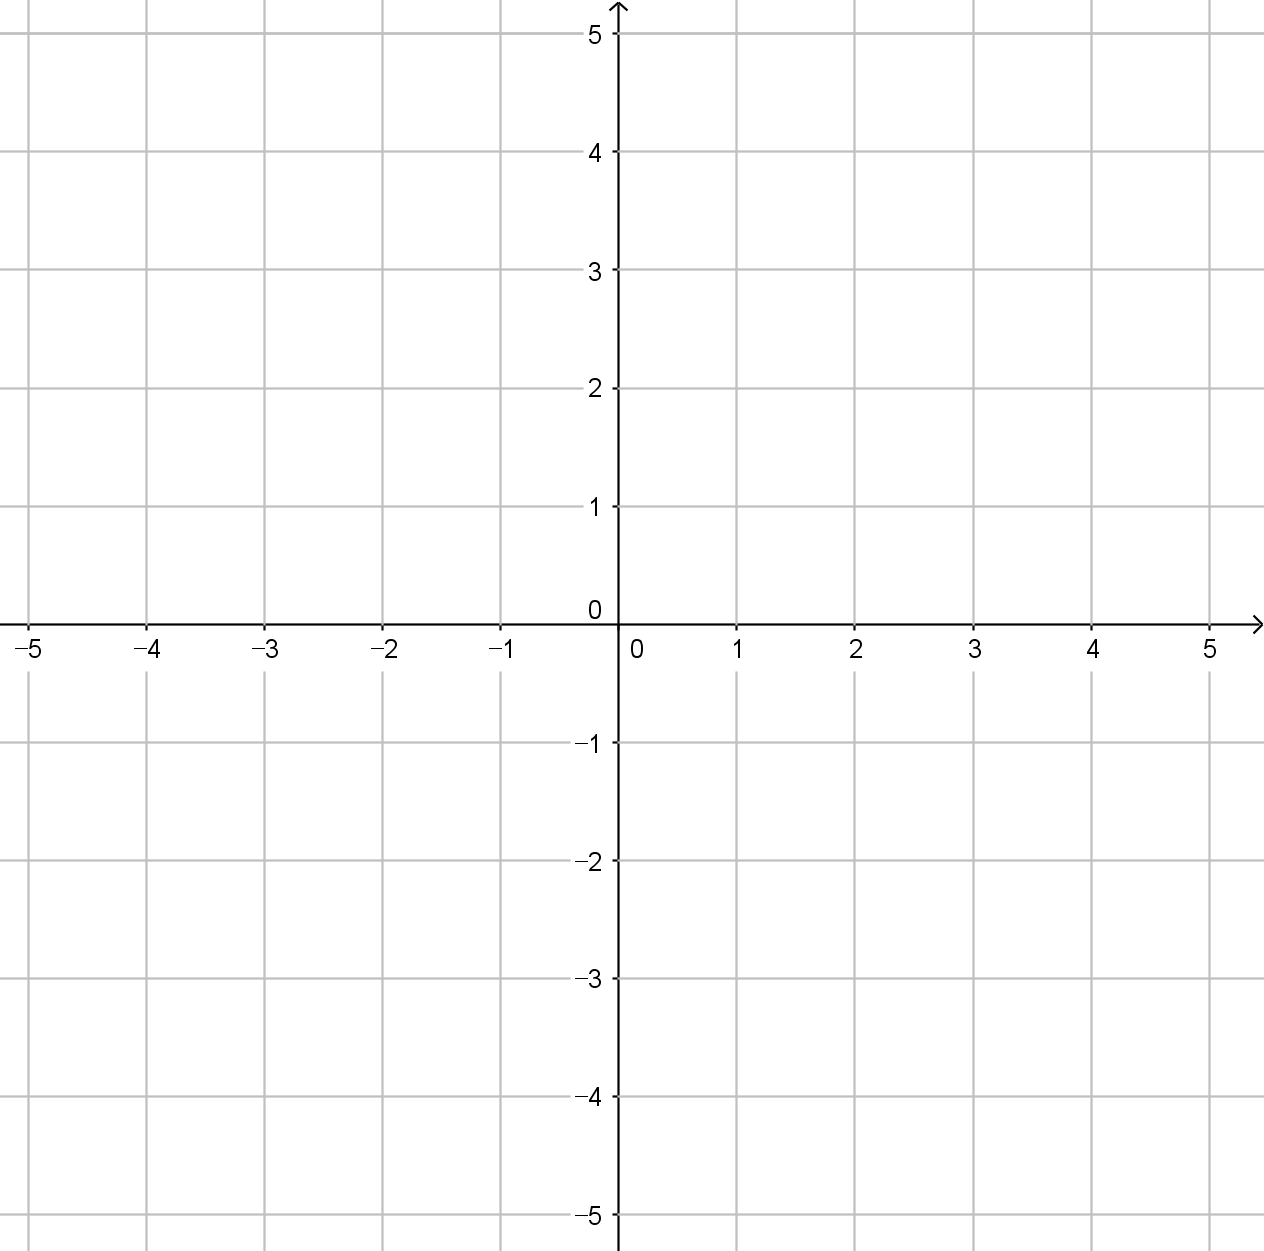
\includegraphics[width=0.9\textwidth]{55}
\end{minipage}\bigskip\bigskip\par
\begin{minipage}{0.45\textwidth}\centering
\(y=\frac23x+2\)
\par\bigskip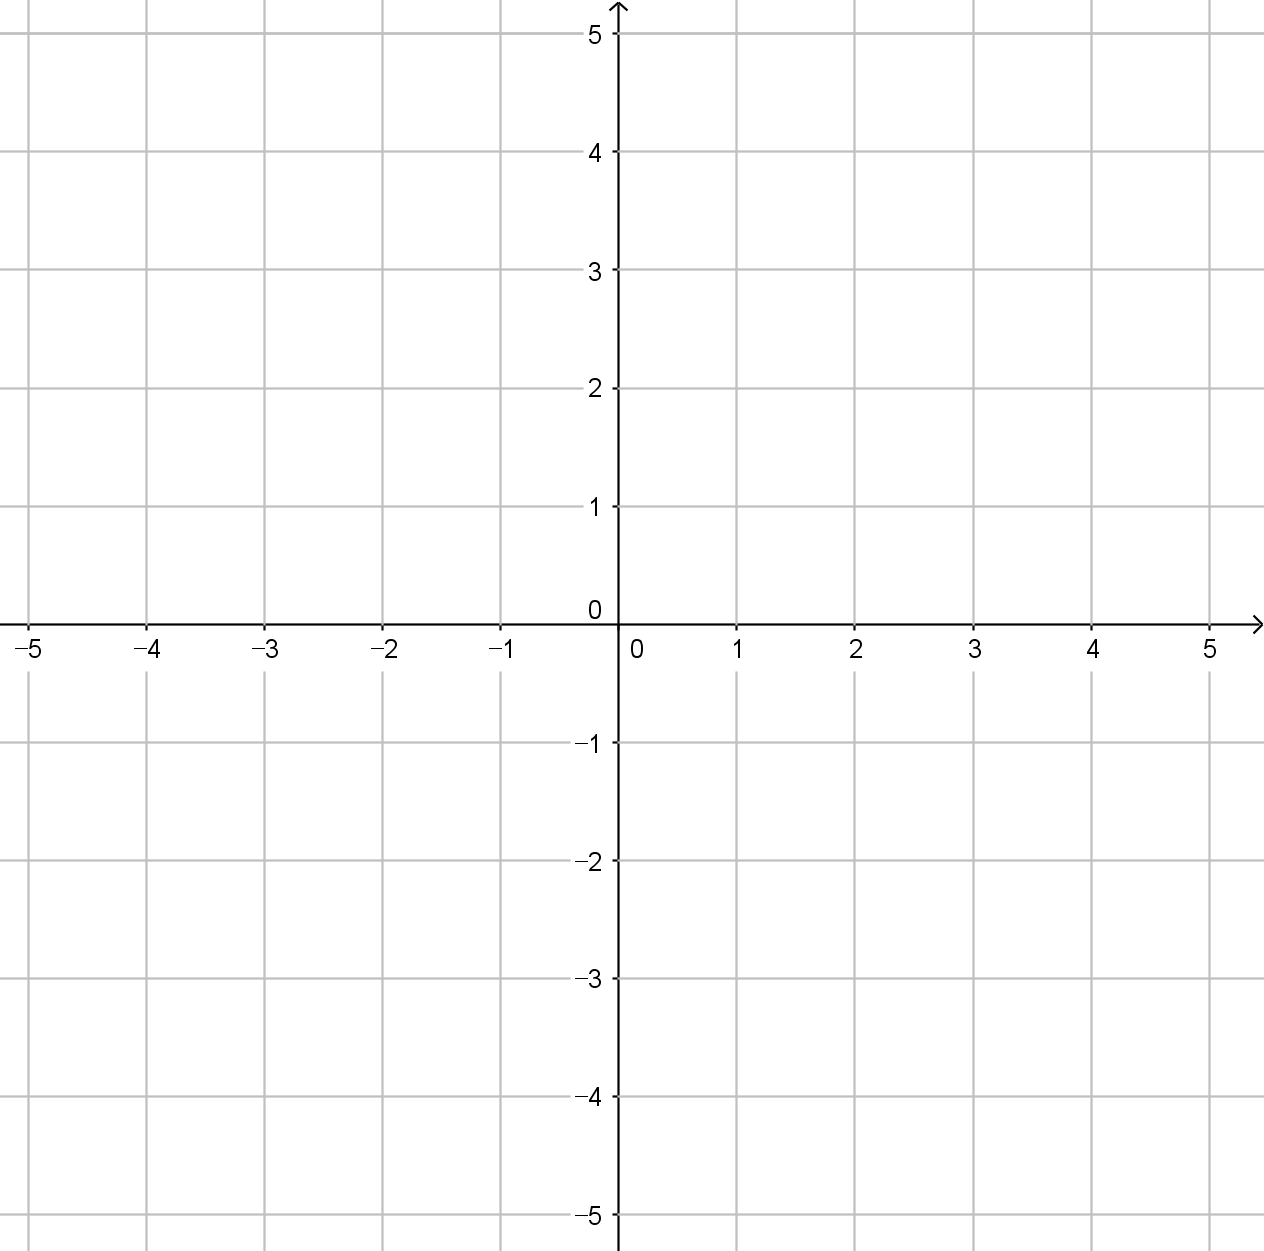
\includegraphics[width=0.9\textwidth]{55}
\end{minipage}
\begin{minipage}{0.45\textwidth}\centering
\(y=-\frac23x+1\)
\par\bigskip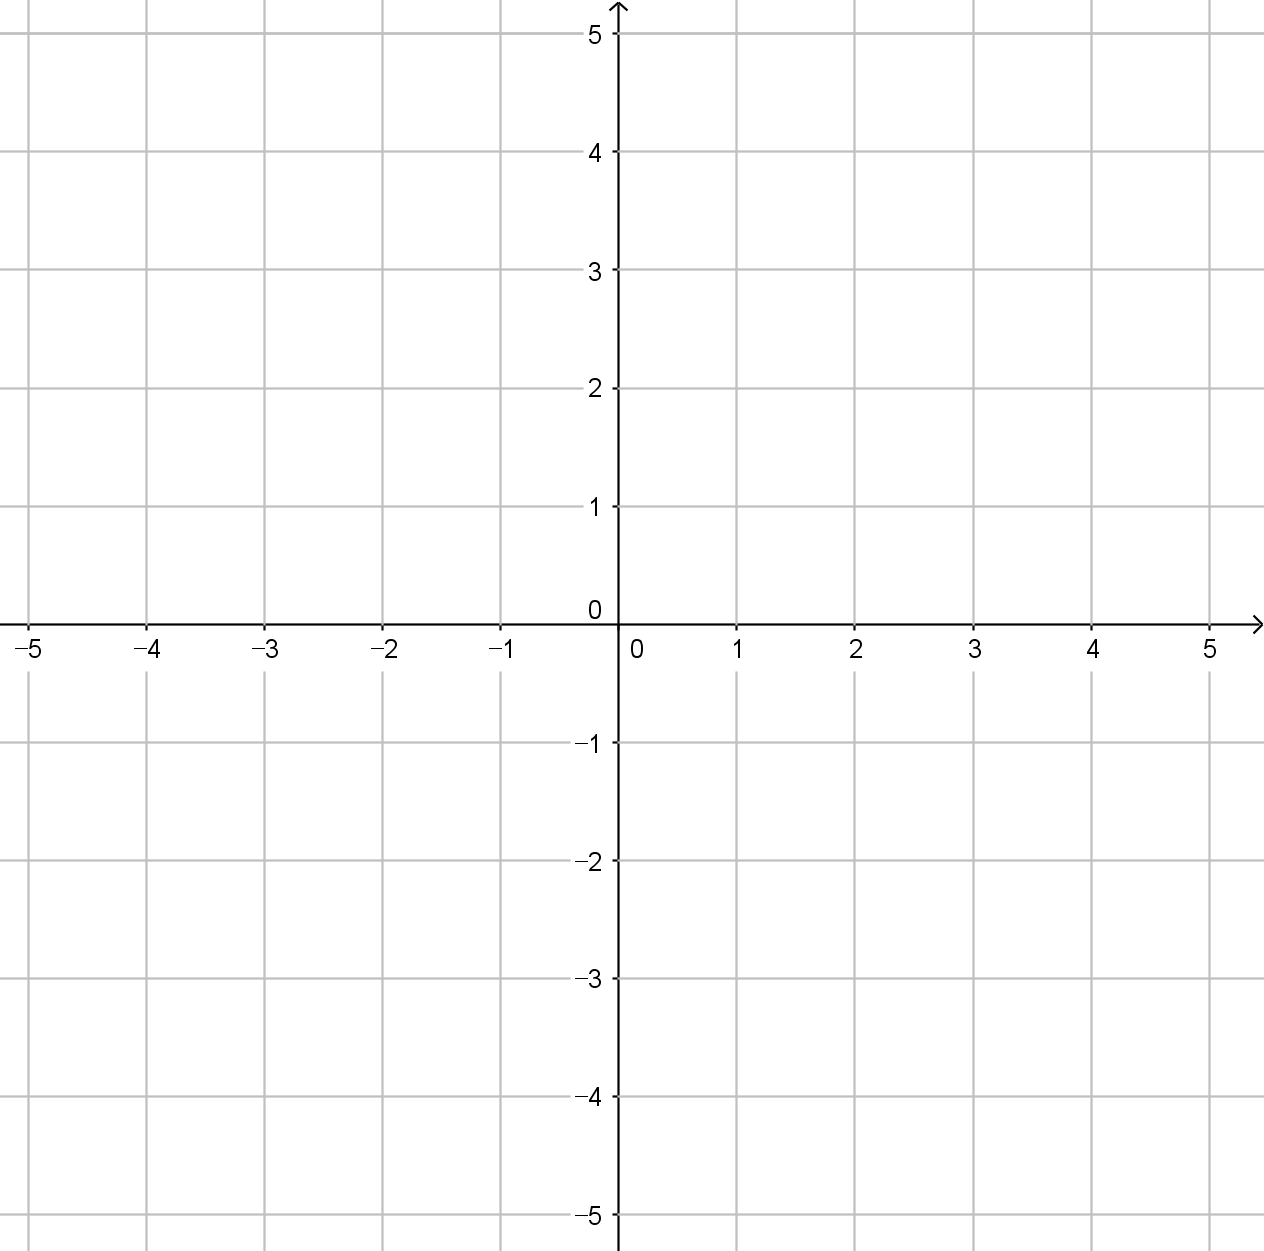
\includegraphics[width=0.9\textwidth]{55}
\end{minipage}\bigskip\bigskip\par


\clearpage
\begin{minipage}{0.45\textwidth}\centering
\(y=\frac32x+3\)
\par\bigskip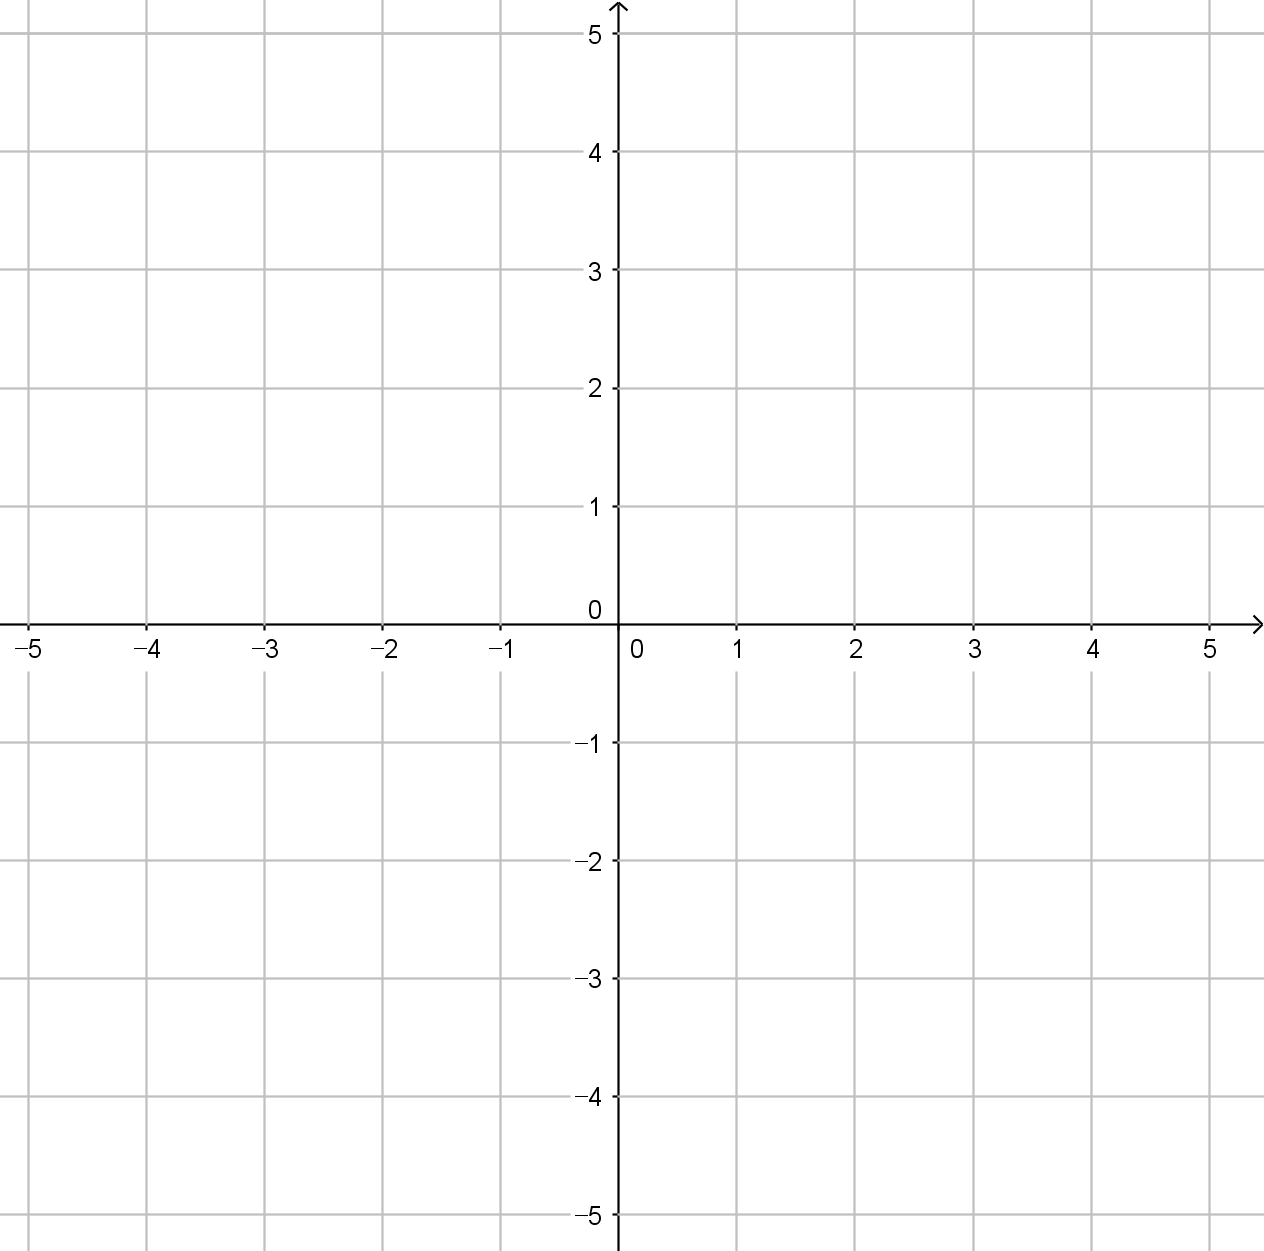
\includegraphics[width=0.9\textwidth]{55}
\end{minipage}
\begin{minipage}{0.45\textwidth}\centering
\(y=-\frac34x\)
\par\bigskip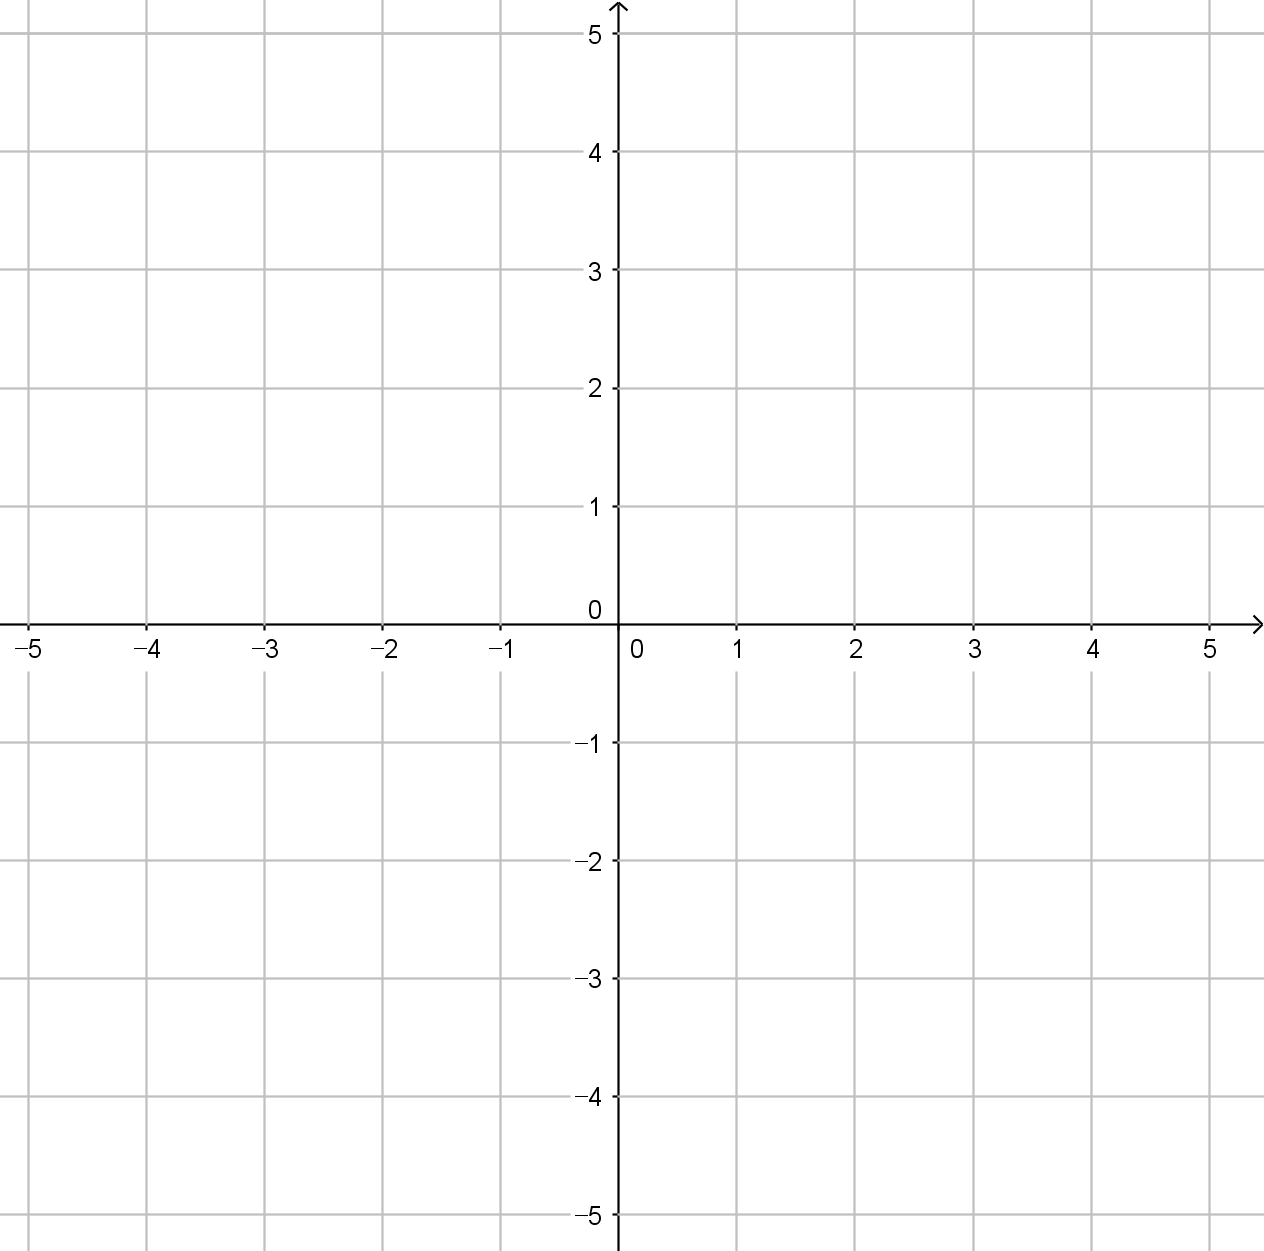
\includegraphics[width=0.9\textwidth]{55}
\end{minipage}\bigskip\bigskip\par
\begin{minipage}{0.45\textwidth}\centering
\(x+y=1\)
\par\bigskip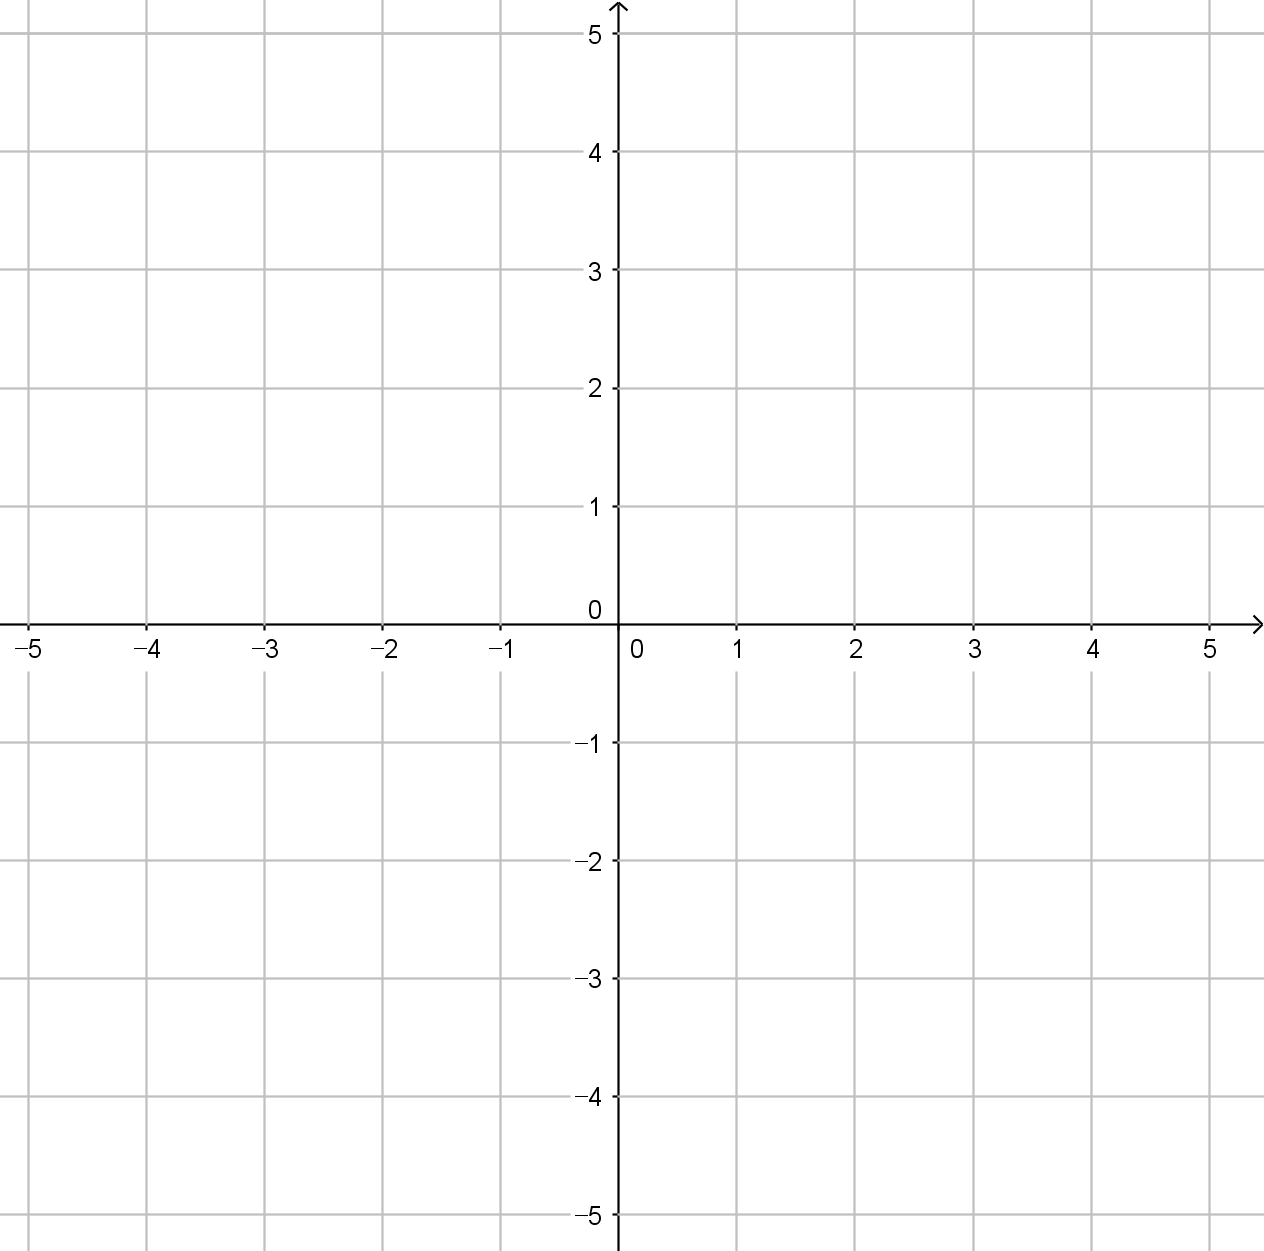
\includegraphics[width=0.9\textwidth]{55}
\end{minipage}
\begin{minipage}{0.45\textwidth}\centering
\(x+y=-2\)
\par\bigskip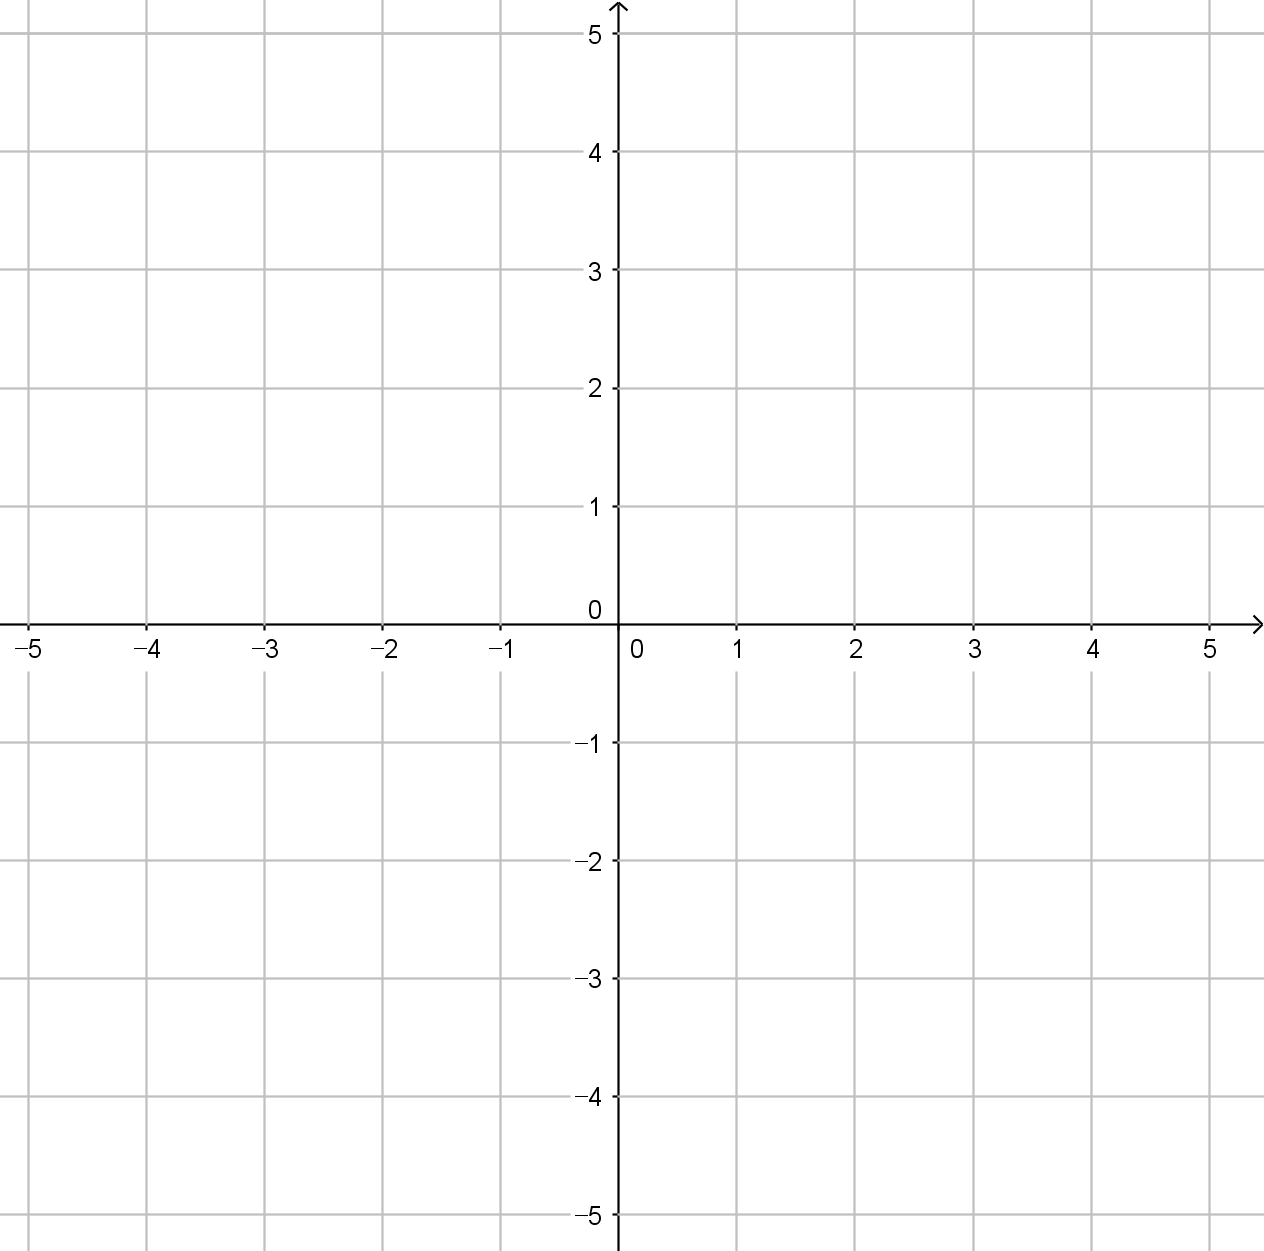
\includegraphics[width=0.9\textwidth]{55}
\end{minipage}\bigskip\bigskip\par
\begin{minipage}{0.45\textwidth}\centering
\(2x+y+2=0\)
\par\bigskip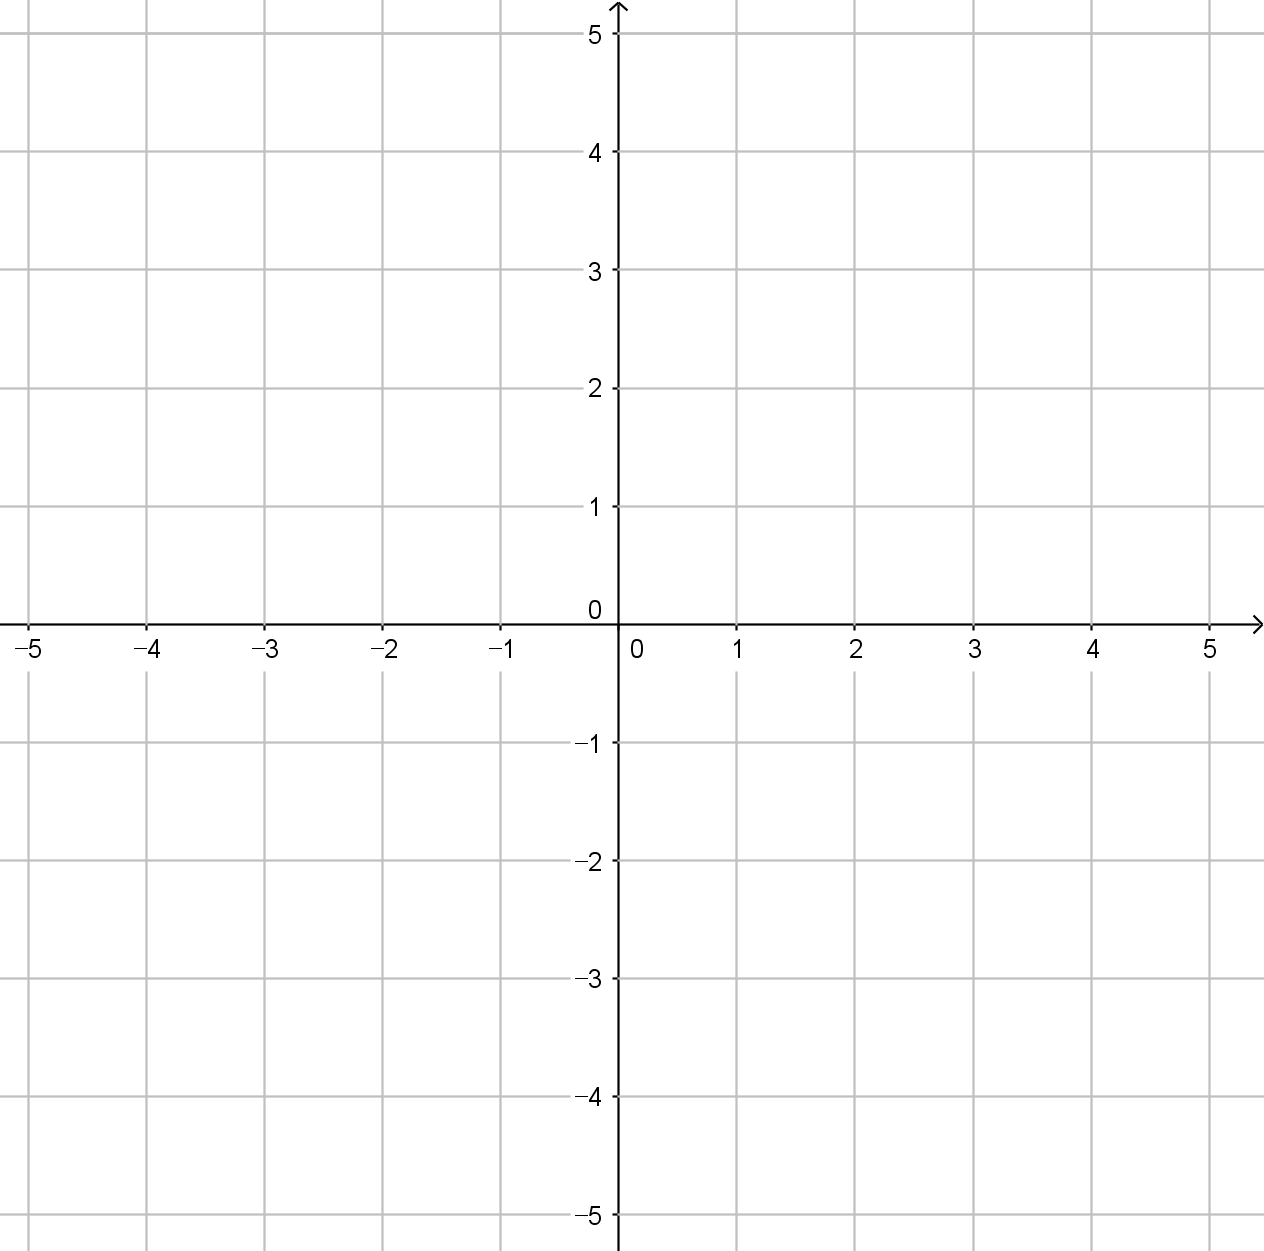
\includegraphics[width=0.9\textwidth]{55}
\end{minipage}
\begin{minipage}{0.45\textwidth}\centering
\(3x-2y+6=0\)
\par\bigskip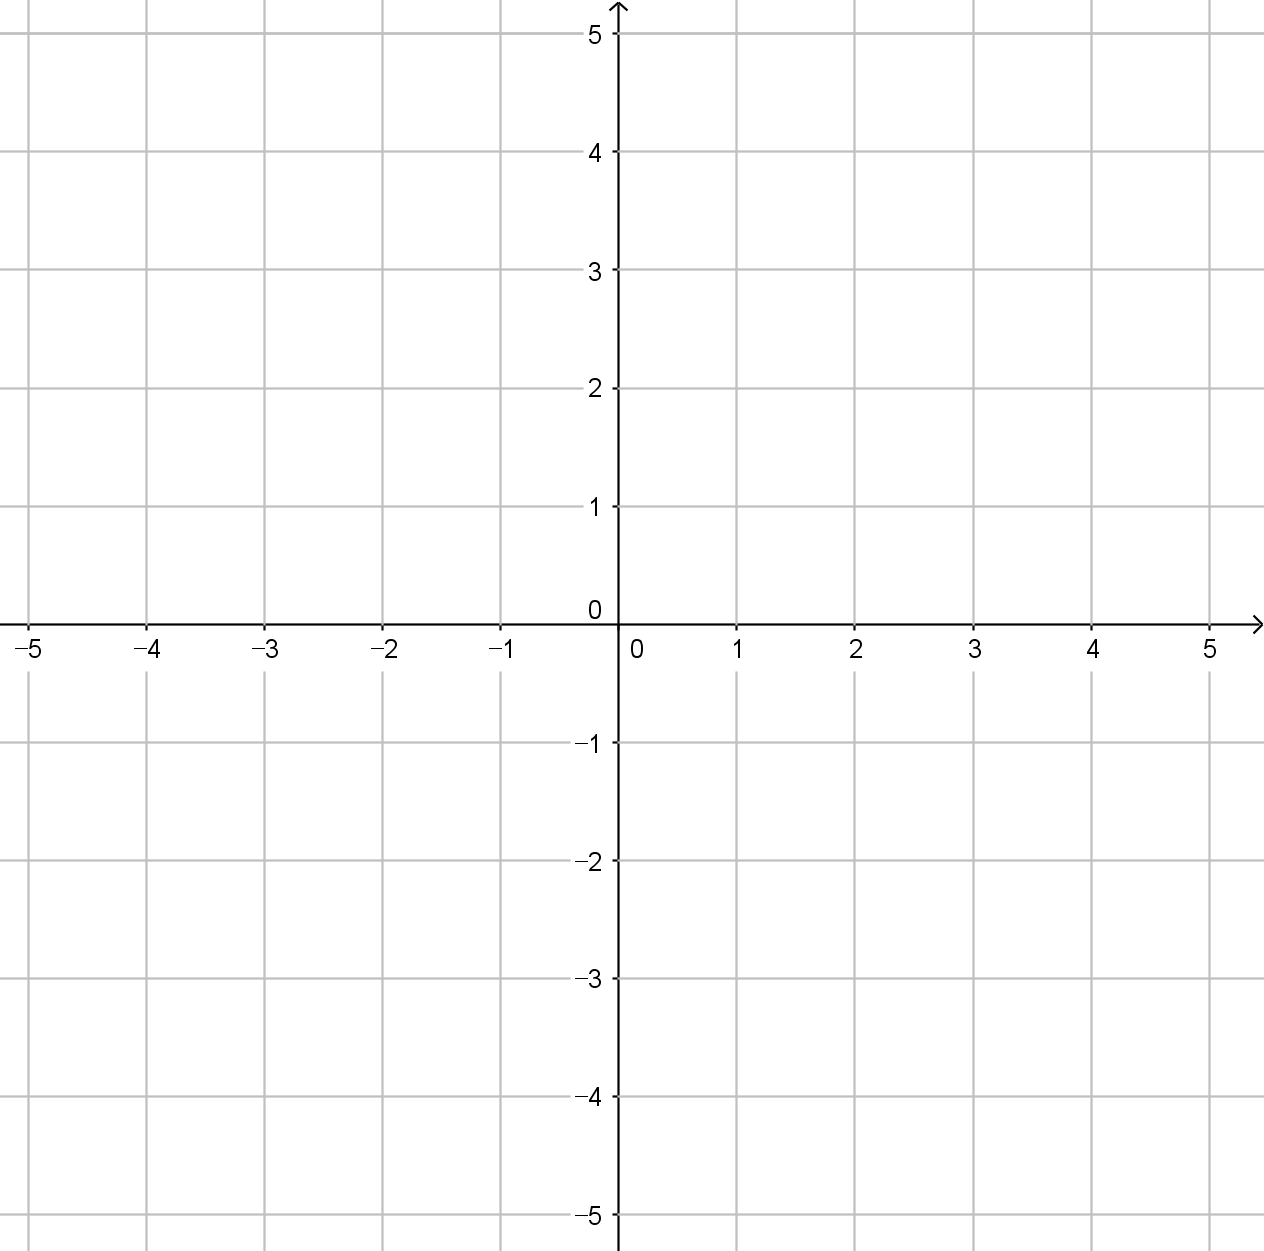
\includegraphics[width=0.9\textwidth]{55}
\end{minipage}\bigskip\bigskip\par


\clearpage
\begin{minipage}{0.45\textwidth}\centering
\(y=3\)
\par\bigskip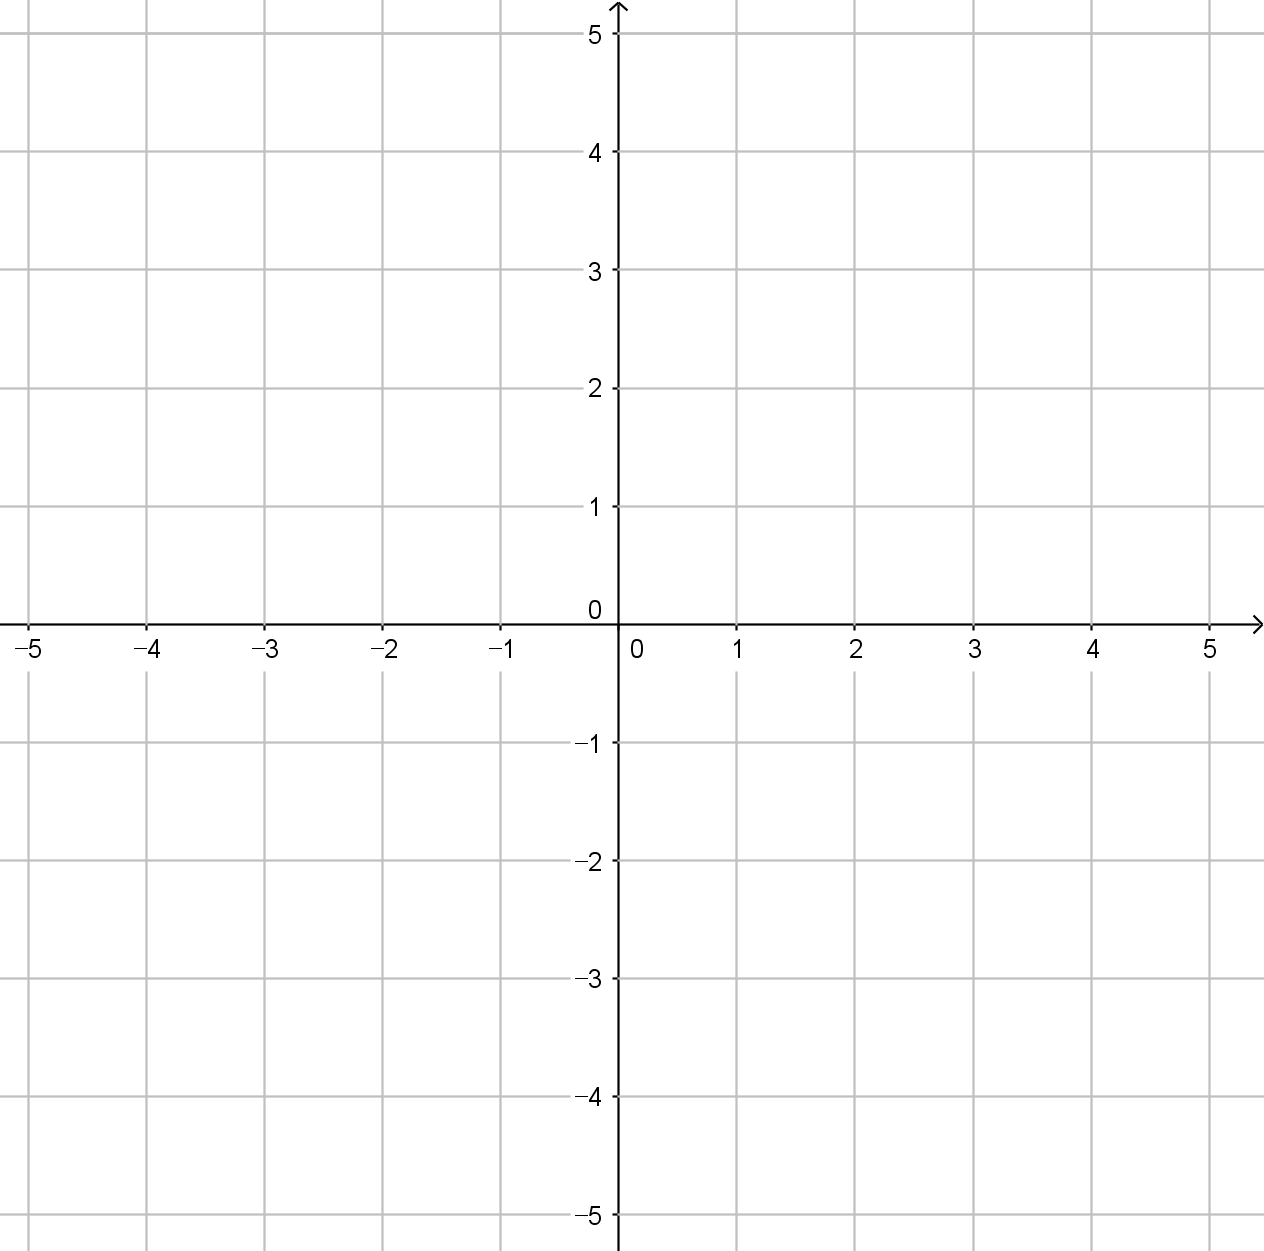
\includegraphics[width=0.9\textwidth]{55}
\end{minipage}
\begin{minipage}{0.45\textwidth}\centering
\(y=-1\)
\par\bigskip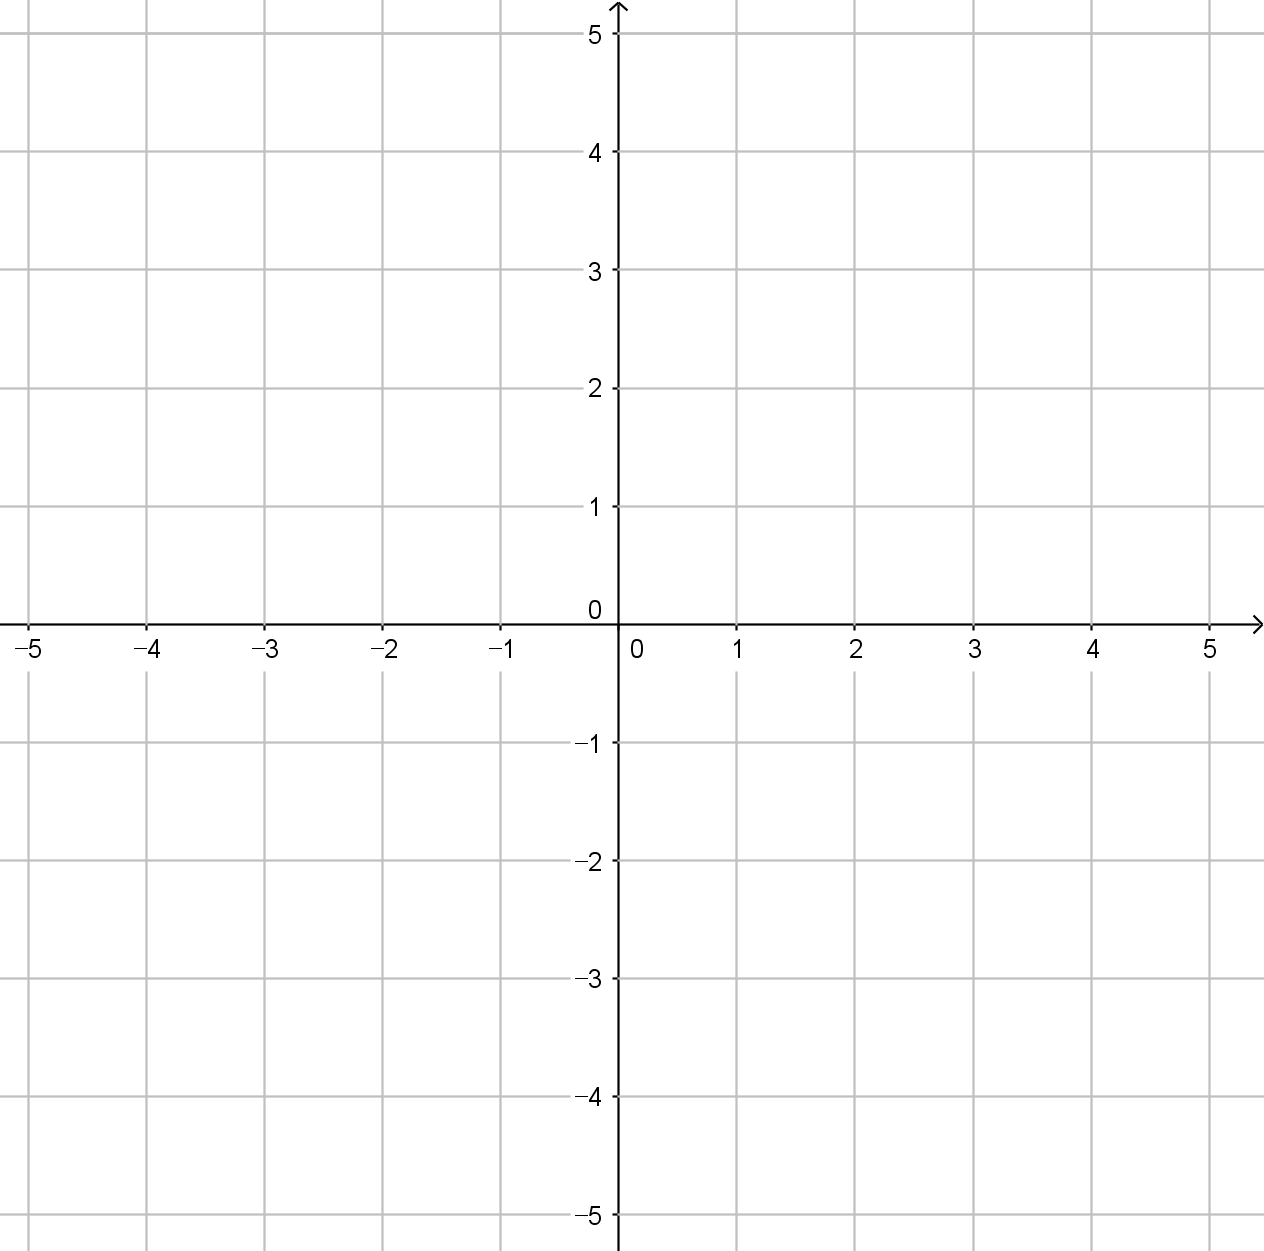
\includegraphics[width=0.9\textwidth]{55}
\end{minipage}\bigskip\bigskip\par
\begin{minipage}{0.45\textwidth}\centering
\(y=0\)
\par\bigskip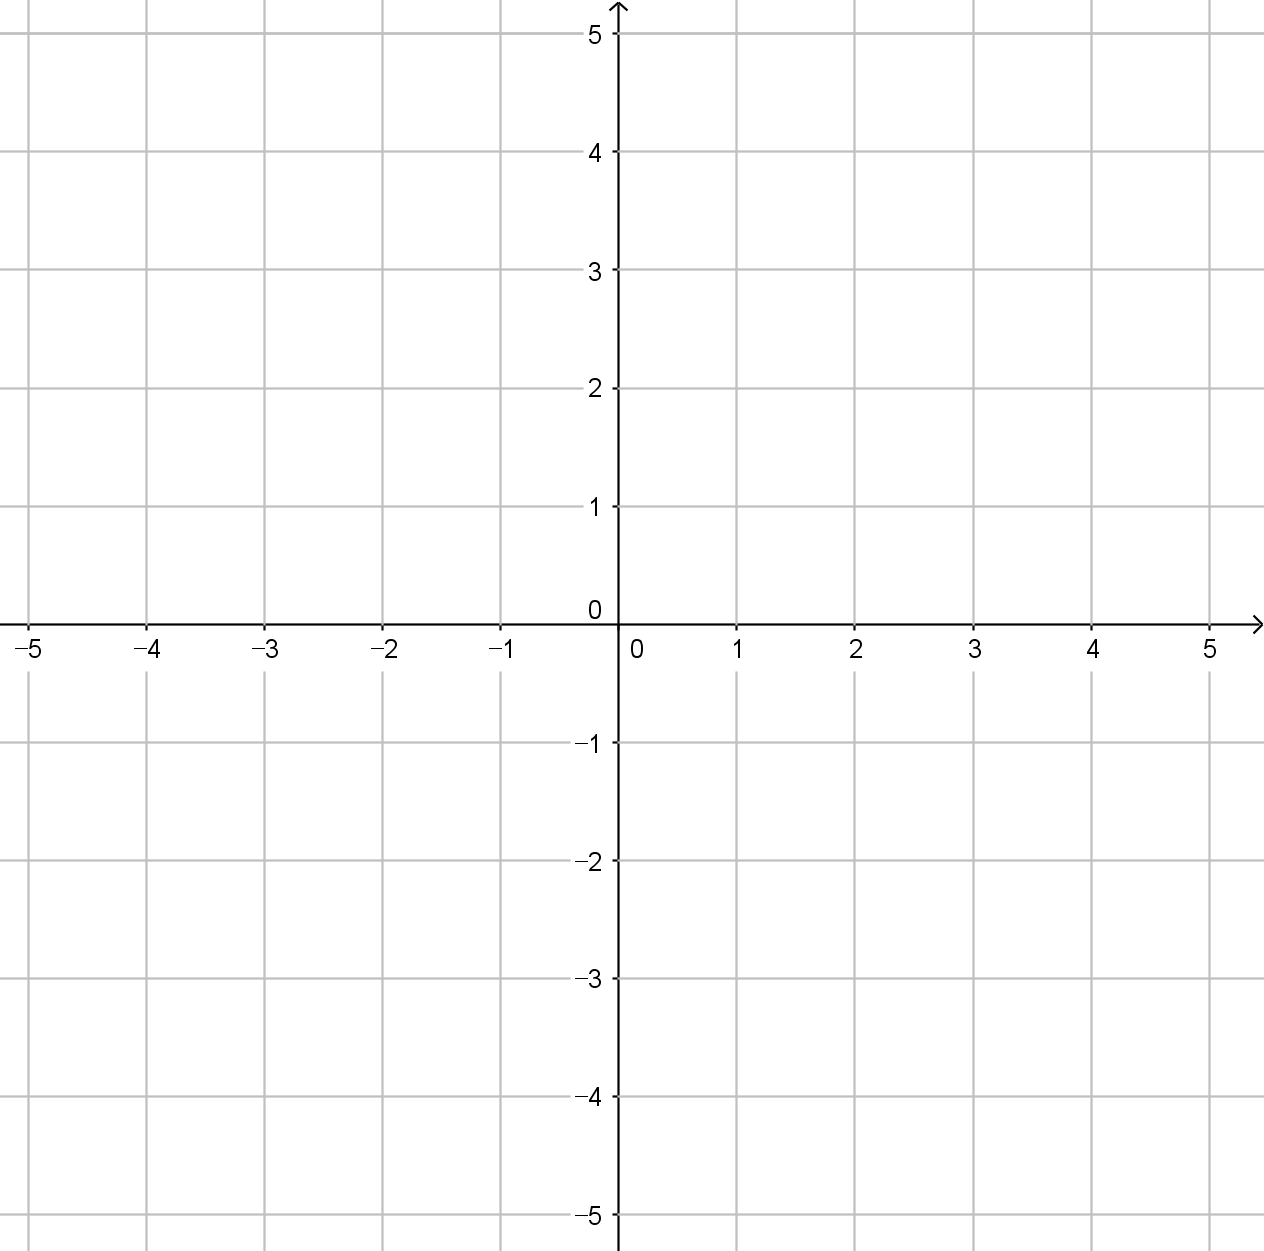
\includegraphics[width=0.9\textwidth]{55}
\end{minipage}
\begin{minipage}{0.45\textwidth}\centering
\(x=1\)
\par\bigskip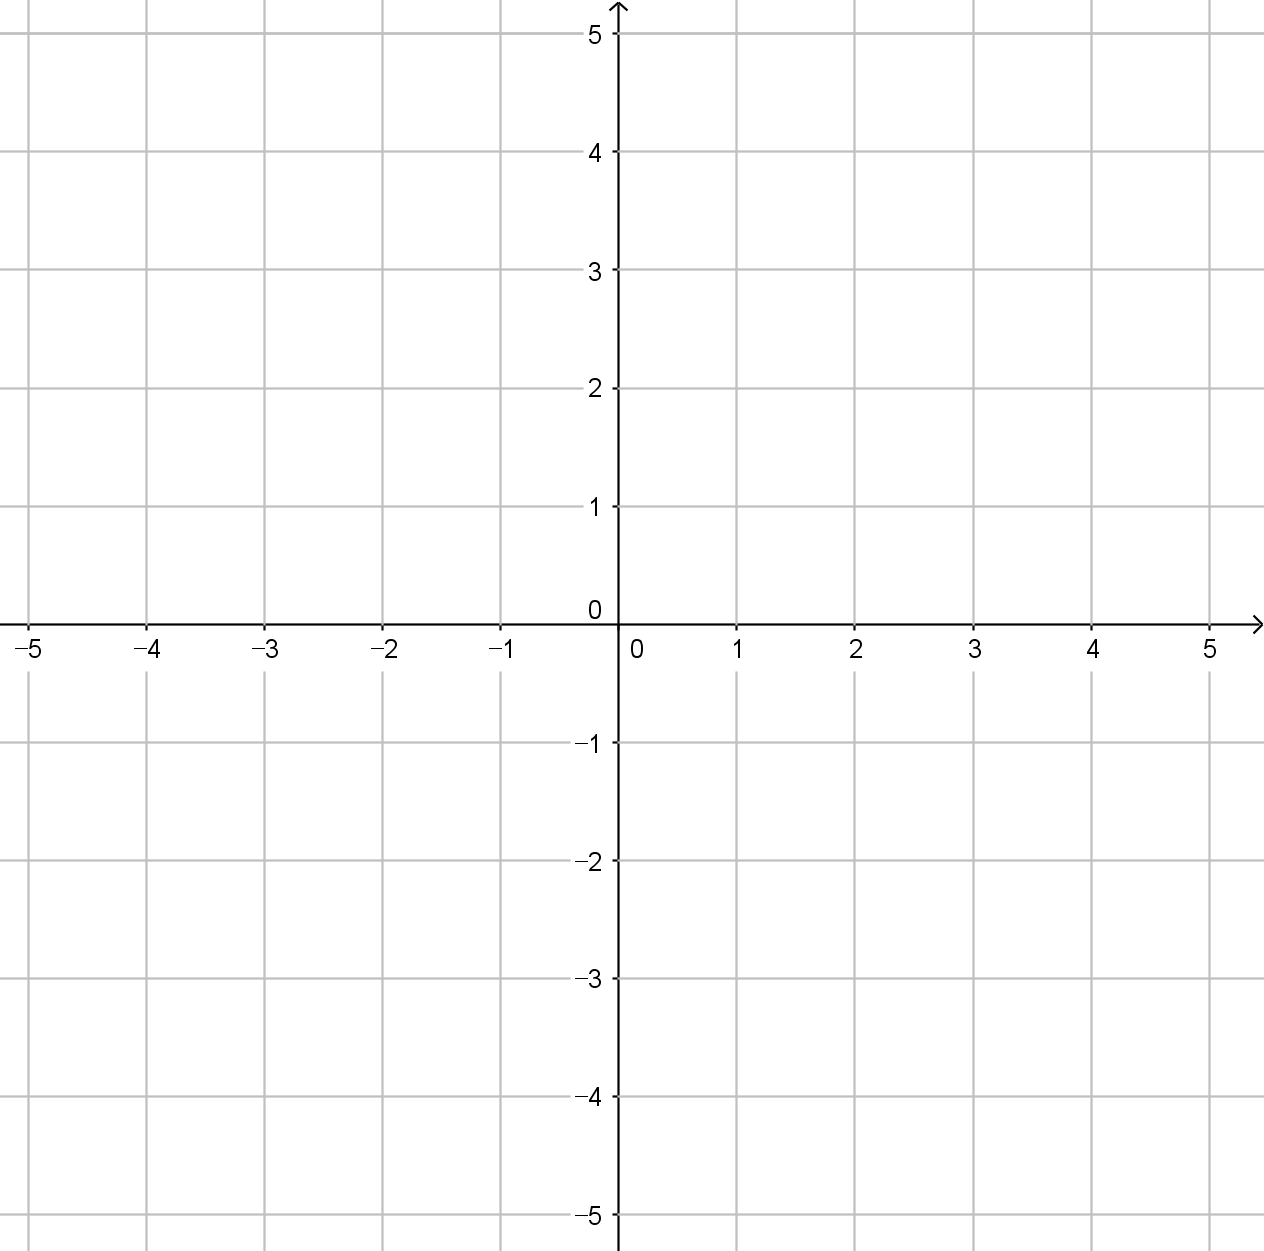
\includegraphics[width=0.9\textwidth]{55}
\end{minipage}\bigskip\bigskip\par
\begin{minipage}{0.45\textwidth}\centering
\(x=-2\)
\par\bigskip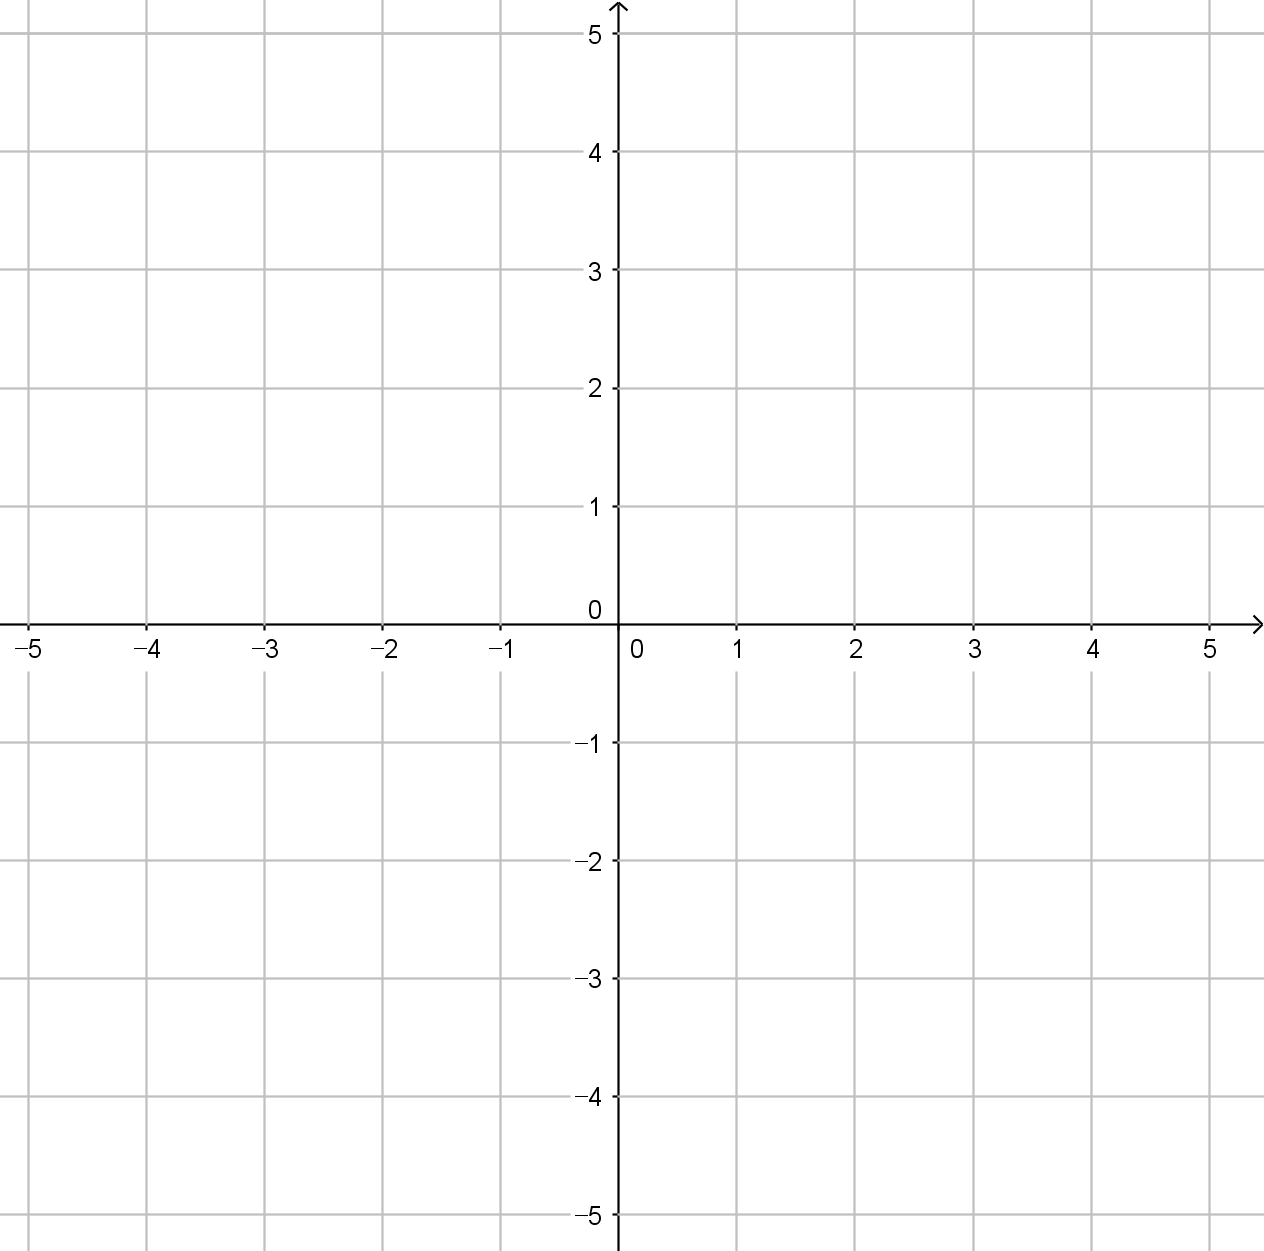
\includegraphics[width=0.9\textwidth]{55}
\end{minipage}
\begin{minipage}{0.45\textwidth}\centering
\(x=0\)
\par\bigskip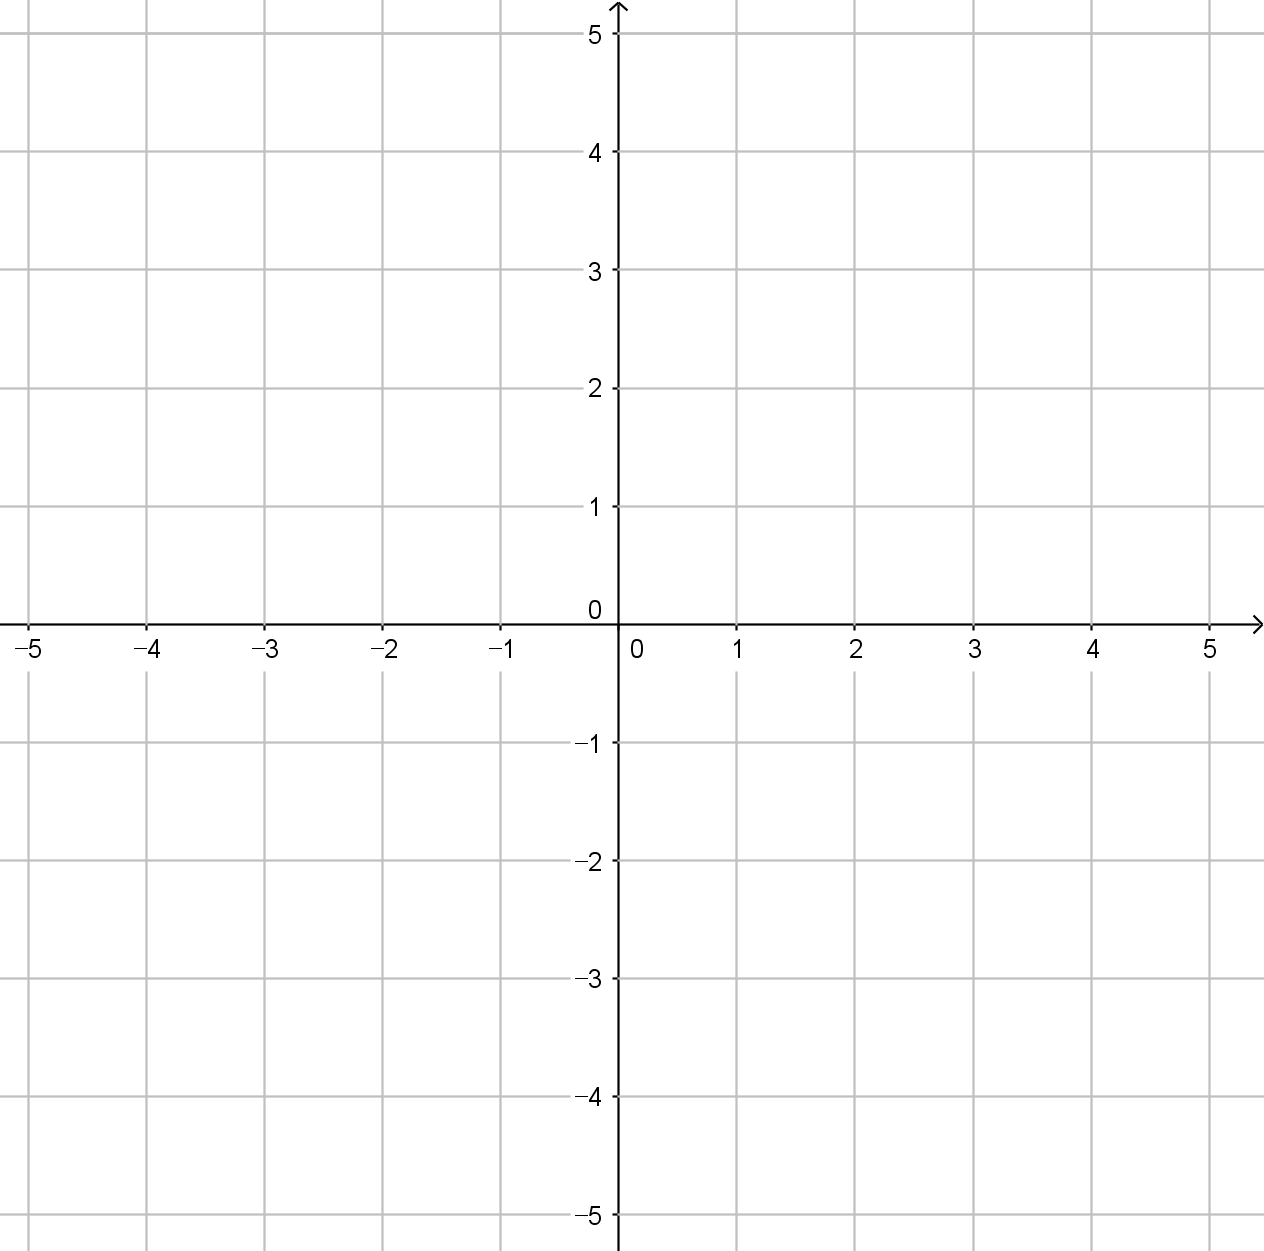
\includegraphics[width=0.9\textwidth]{55}
\end{minipage}\bigskip\bigskip\par


%%
\section*{답}

\begin{minipage}{0.45\textwidth}\centering
\(y=x\)
\par\bigskip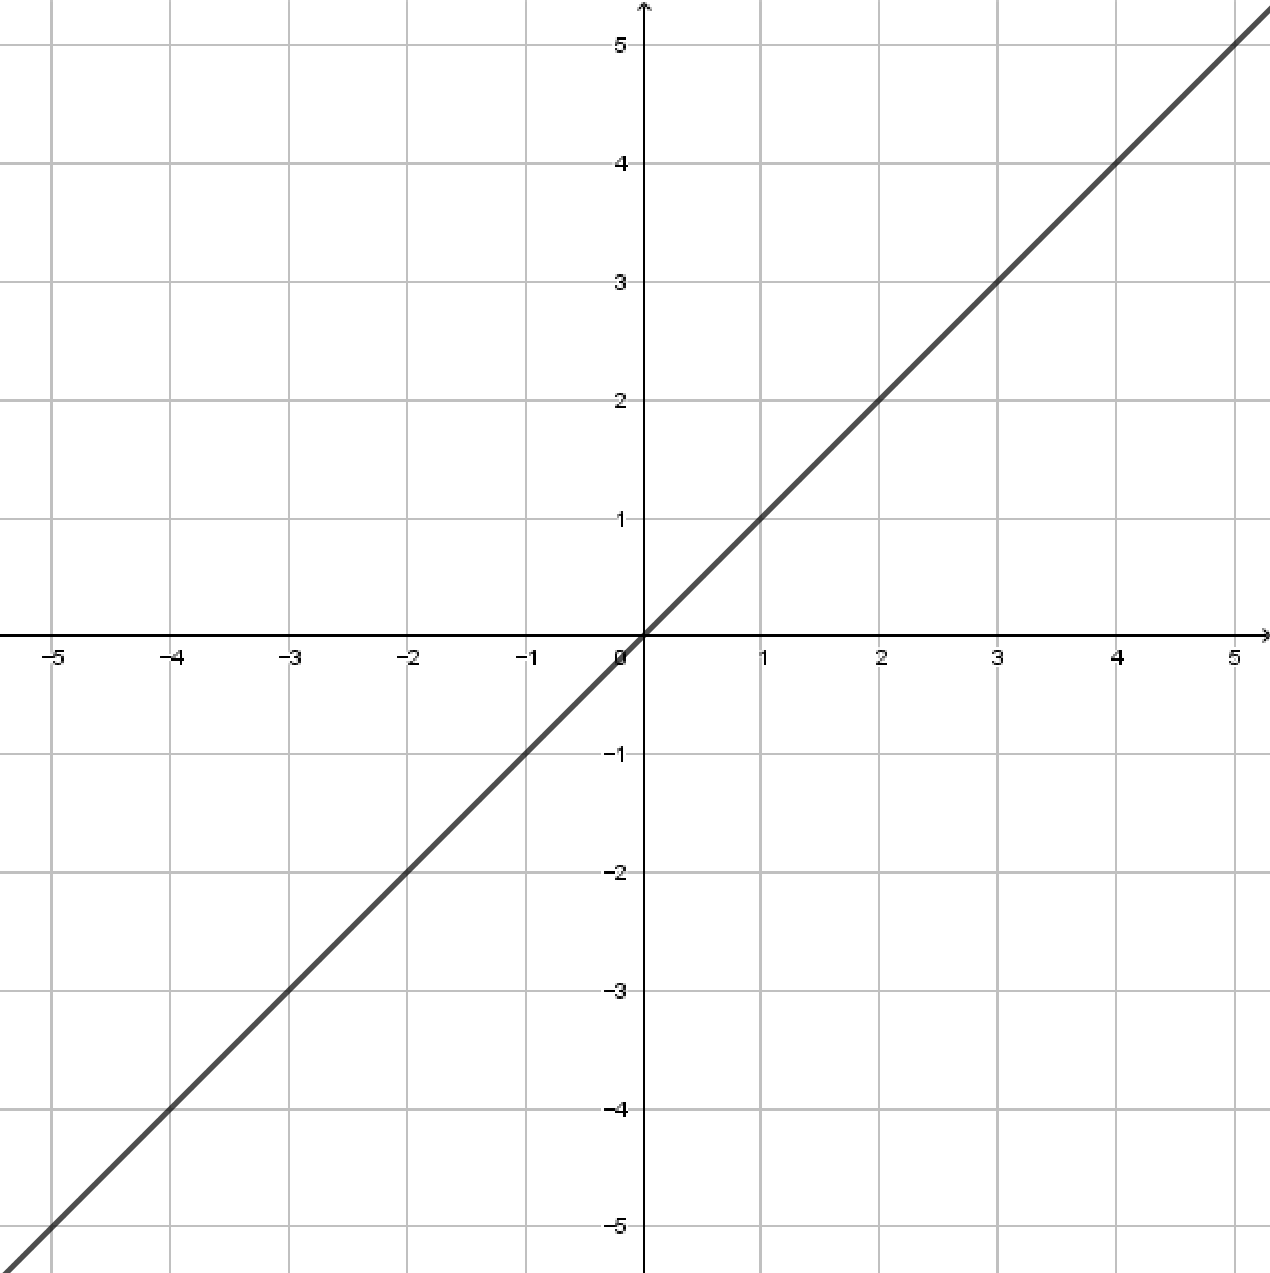
\includegraphics[width=0.9\textwidth]{img/1_line_1}
\end{minipage}
\begin{minipage}{0.45\textwidth}\centering
\(y=-x\)
\par\bigskip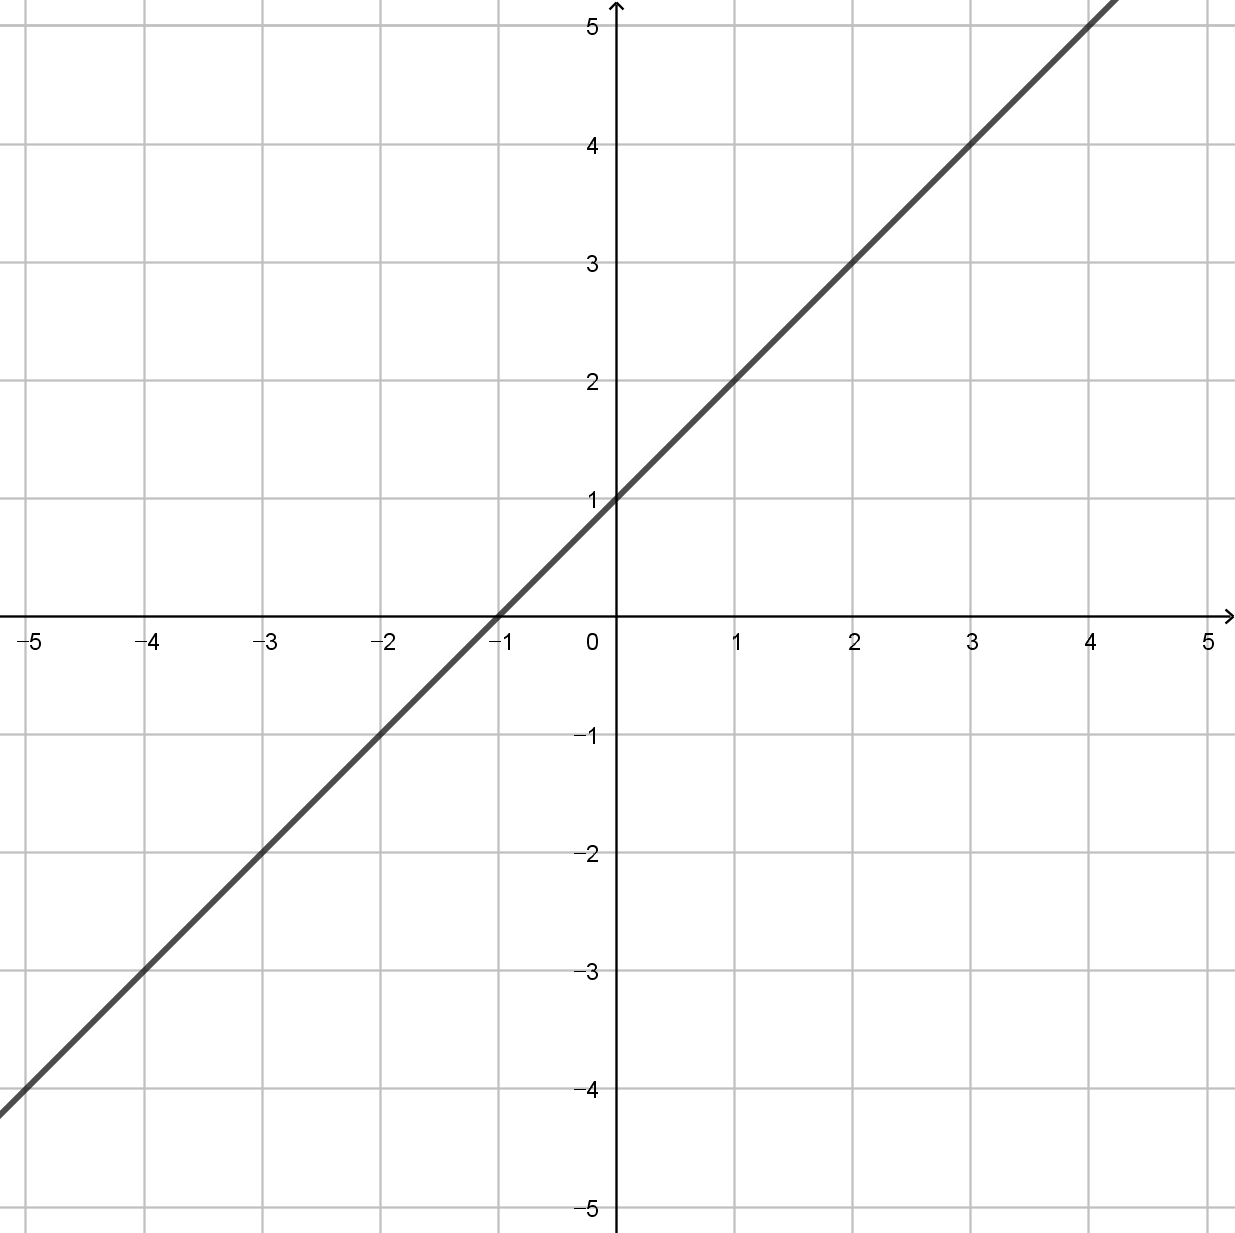
\includegraphics[width=0.9\textwidth]{img/1_line_2}
\end{minipage}\bigskip\bigskip\par
\begin{minipage}{0.45\textwidth}\centering
\(y=2x\)
\par\bigskip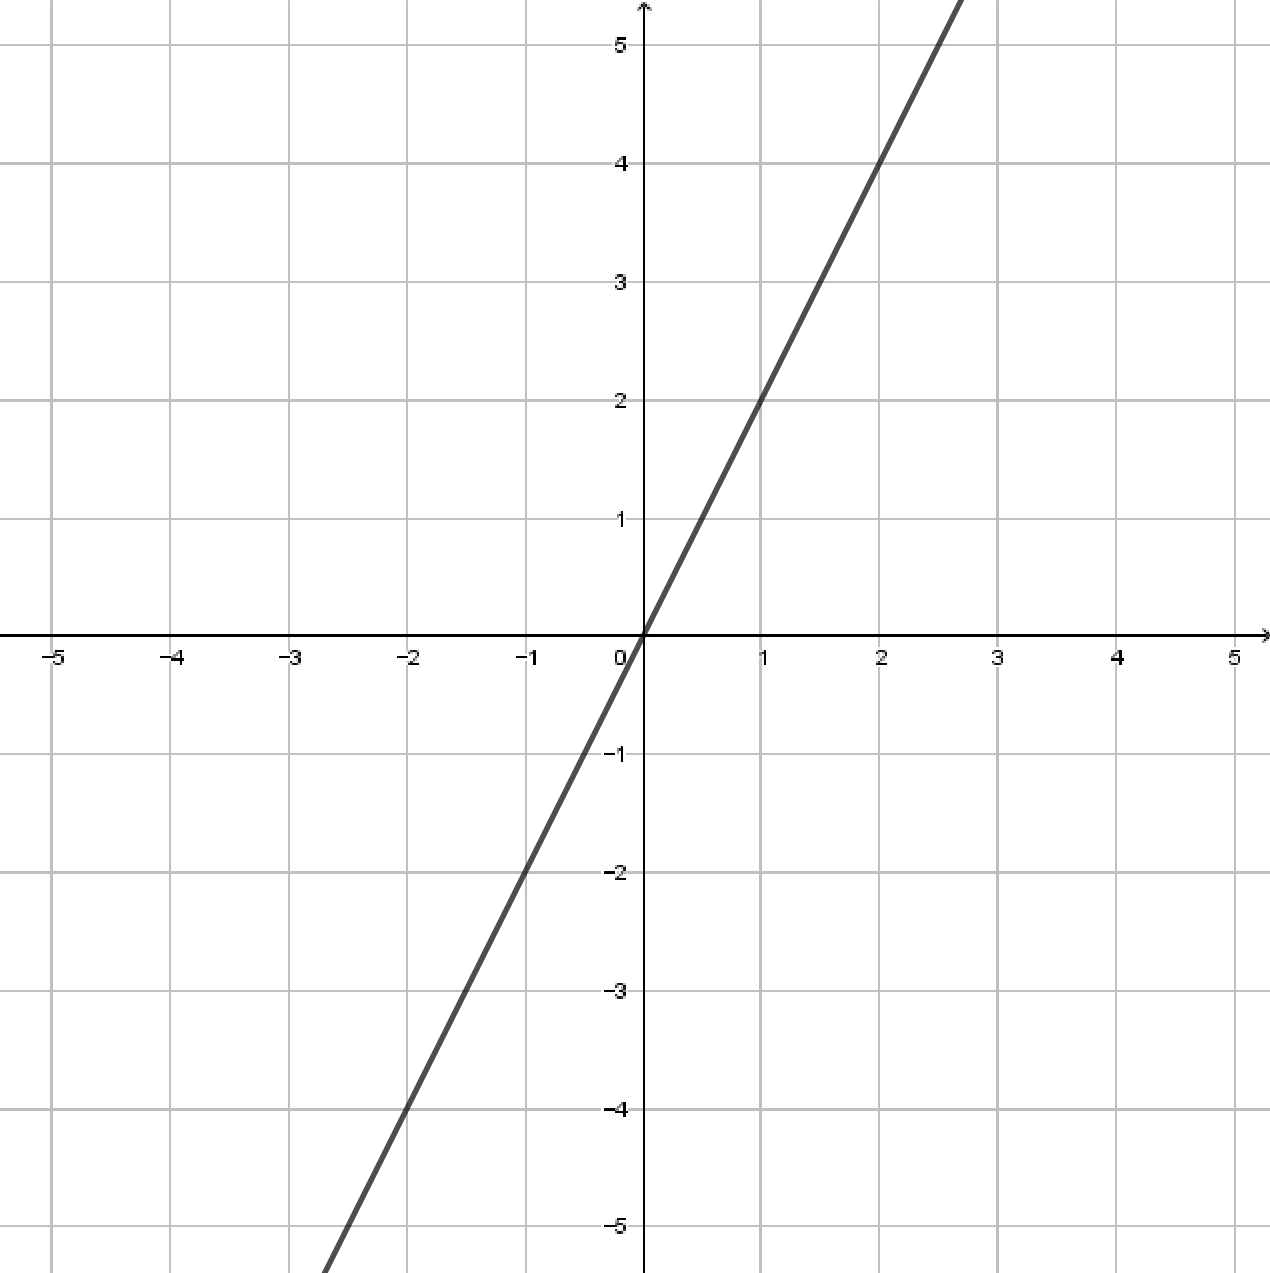
\includegraphics[width=0.9\textwidth]{img/1_line_3}
\end{minipage}
\begin{minipage}{0.45\textwidth}\centering
\(y=-2x\)
\par\bigskip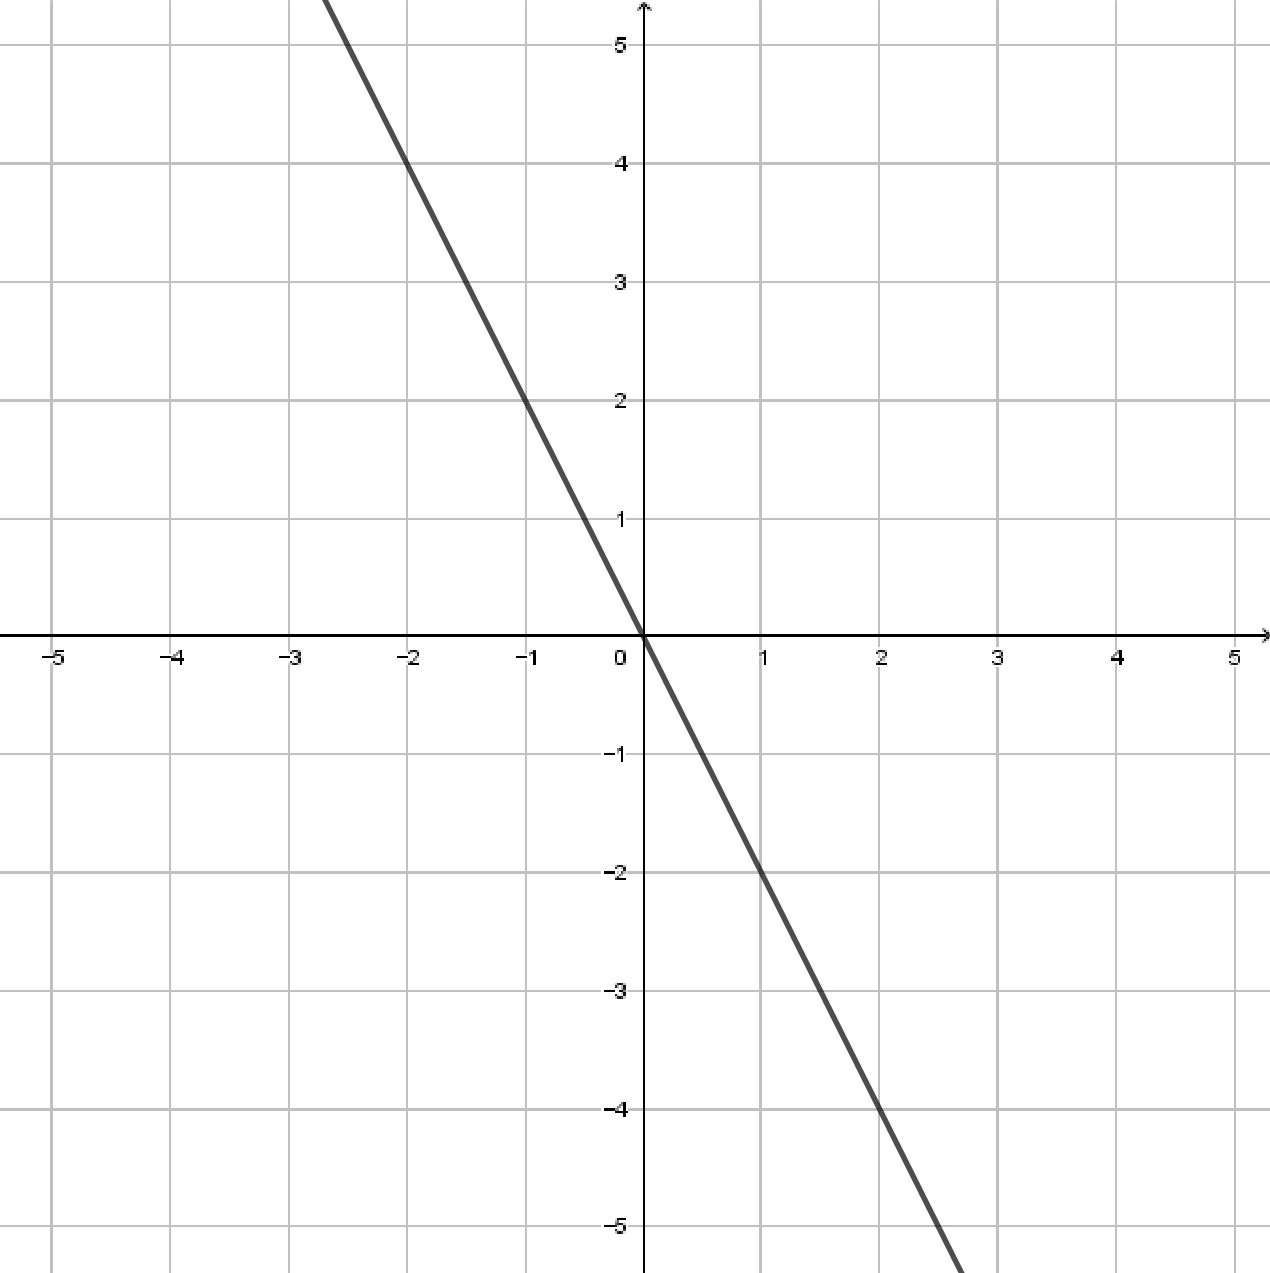
\includegraphics[width=0.9\textwidth]{img/1_line_4}
\end{minipage}\bigskip\bigskip\par

\clearpage
\begin{minipage}{0.45\textwidth}\centering
\(y=x+2\)
\par\bigskip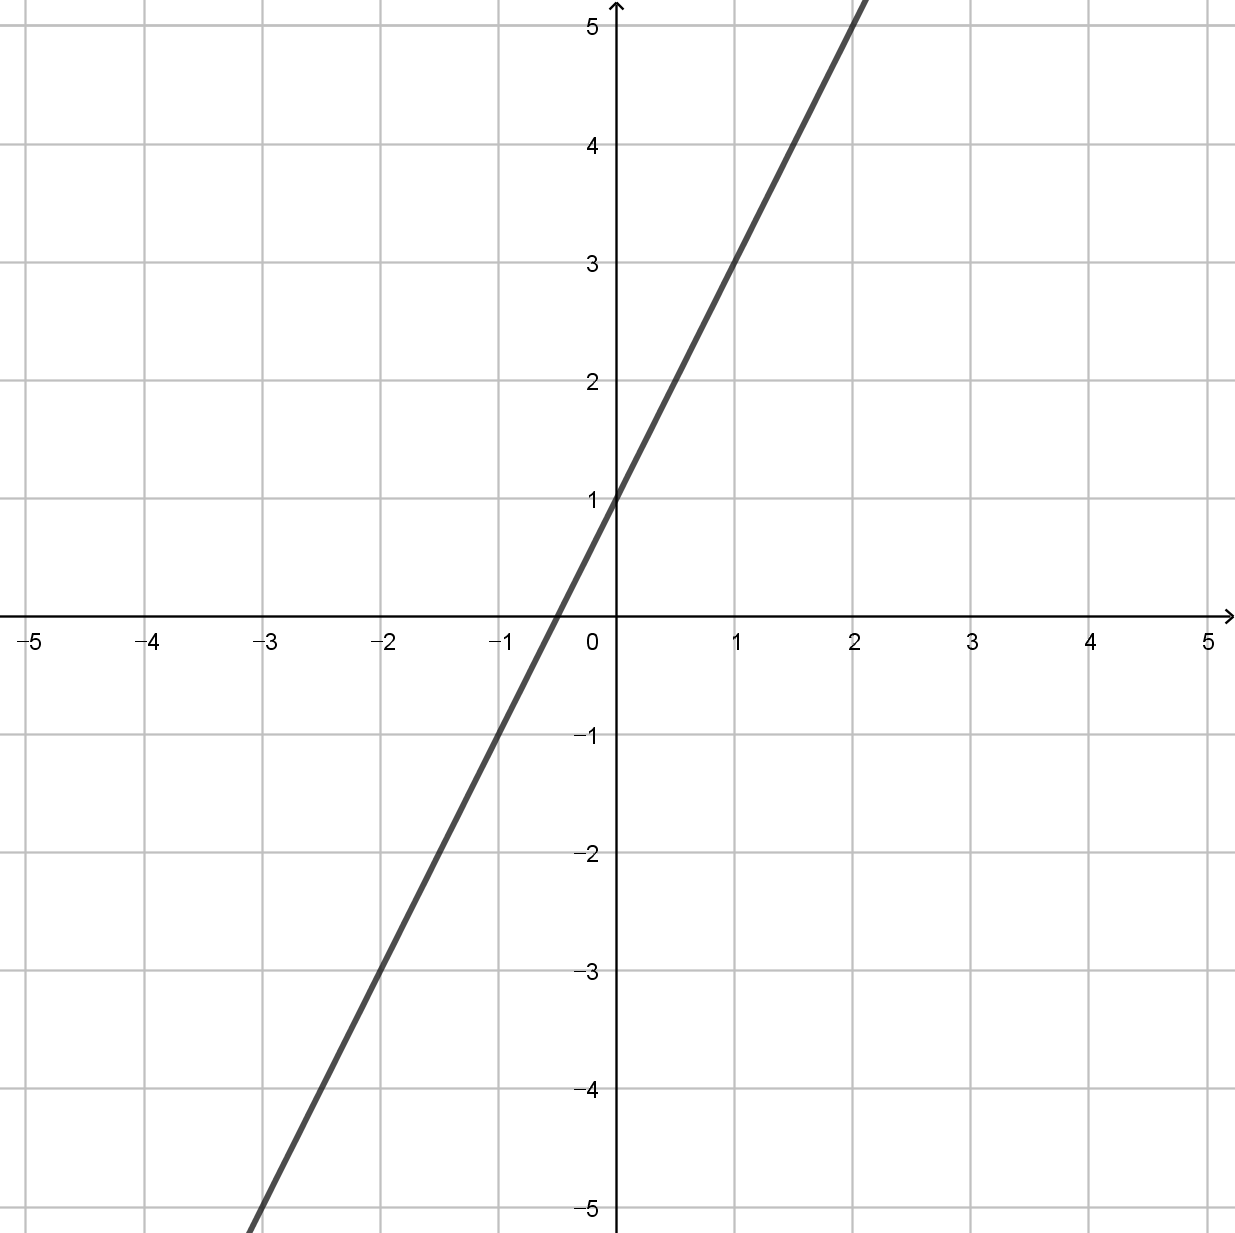
\includegraphics[width=0.9\textwidth]{img/1_line_5}
\end{minipage}
\begin{minipage}{0.45\textwidth}\centering
\(y=x+1\)
\par\bigskip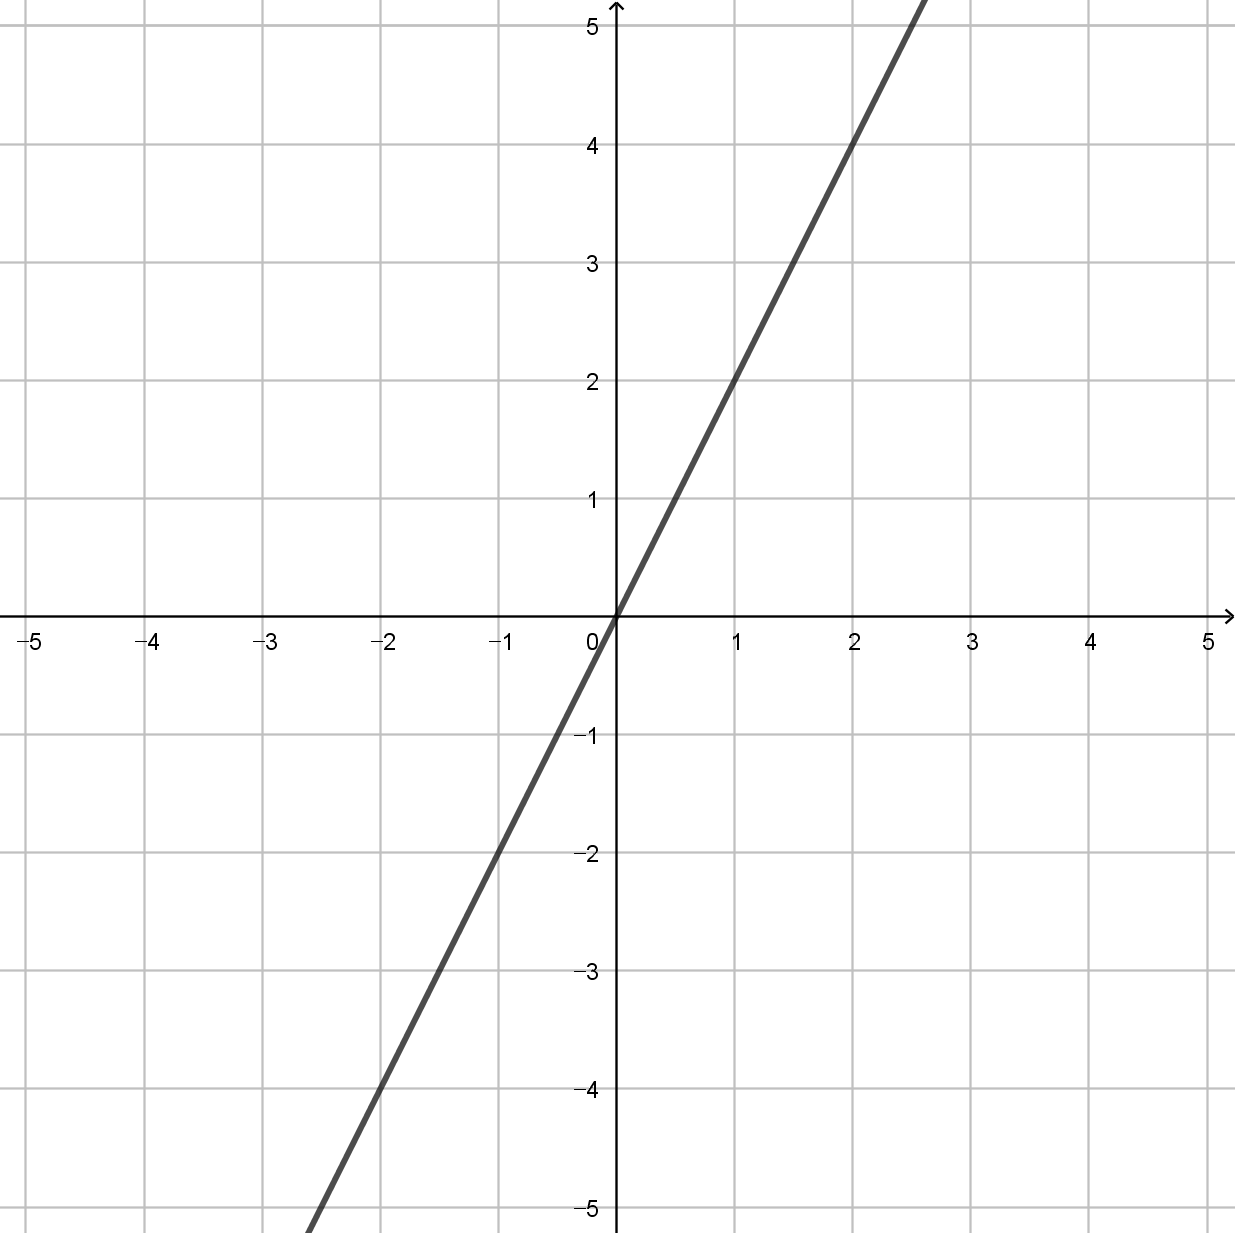
\includegraphics[width=0.9\textwidth]{img/1_line_6}
\end{minipage}\bigskip\bigskip\par
\begin{minipage}{0.45\textwidth}\centering
\(y=x-2\)
\par\bigskip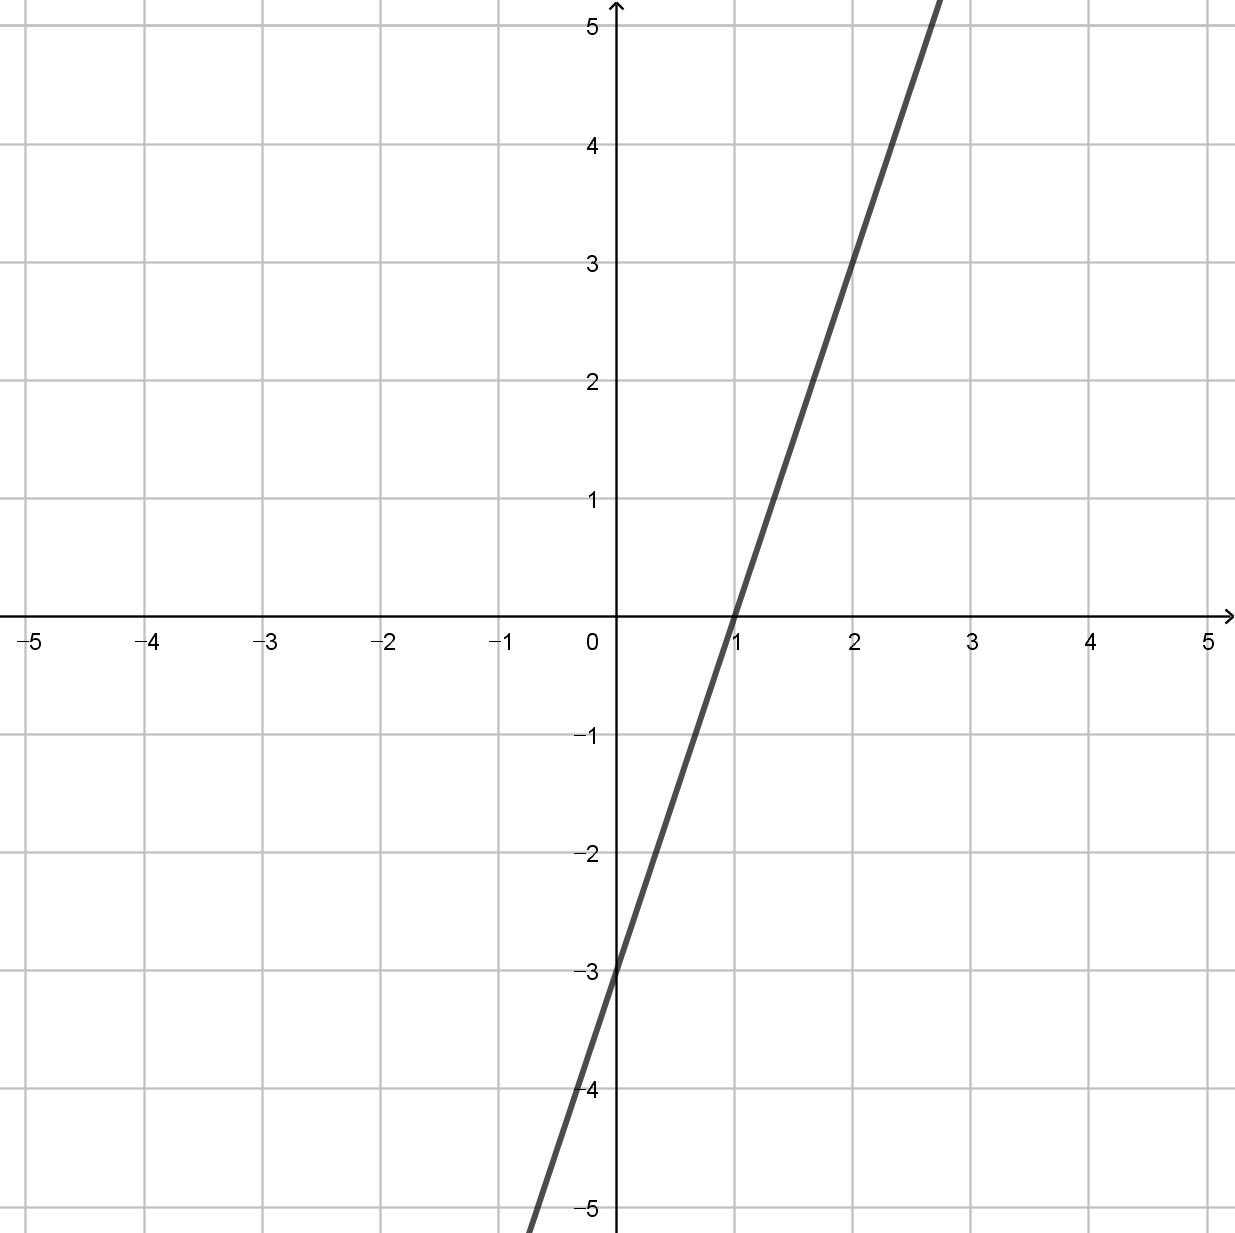
\includegraphics[width=0.9\textwidth]{img/1_line_7}
\end{minipage}
\begin{minipage}{0.45\textwidth}\centering
\(y=2x-2\)
\par\bigskip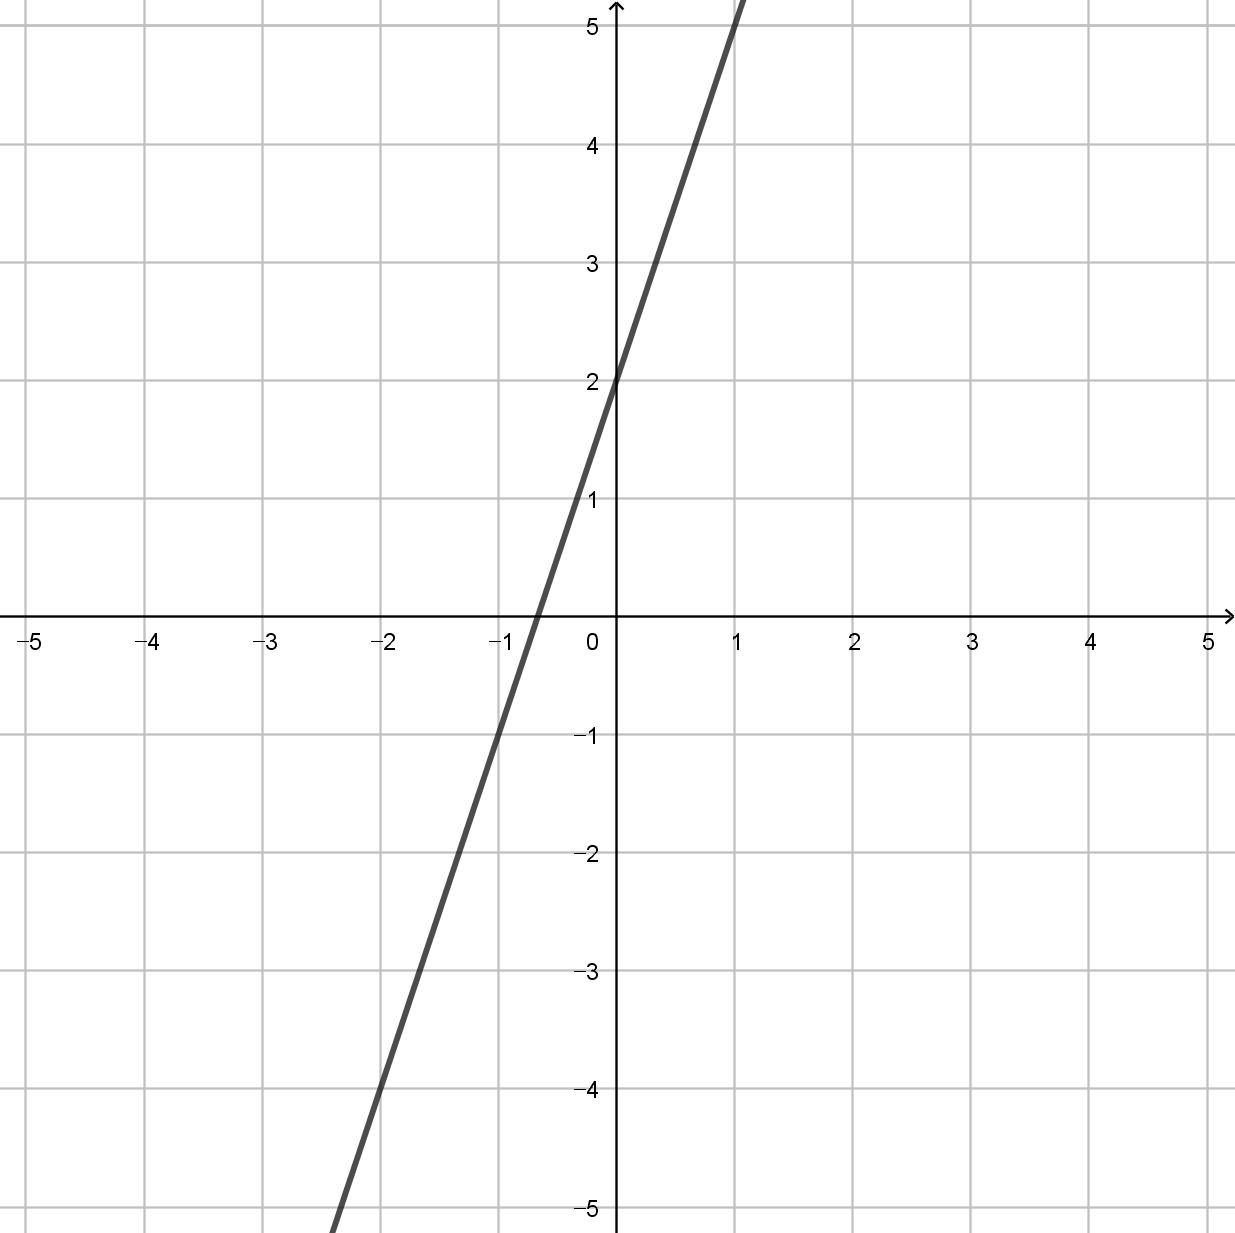
\includegraphics[width=0.9\textwidth]{img/1_line_8}
\end{minipage}\bigskip\bigskip\par
\begin{minipage}{0.45\textwidth}\centering
\(y=2x+1\)
\par\bigskip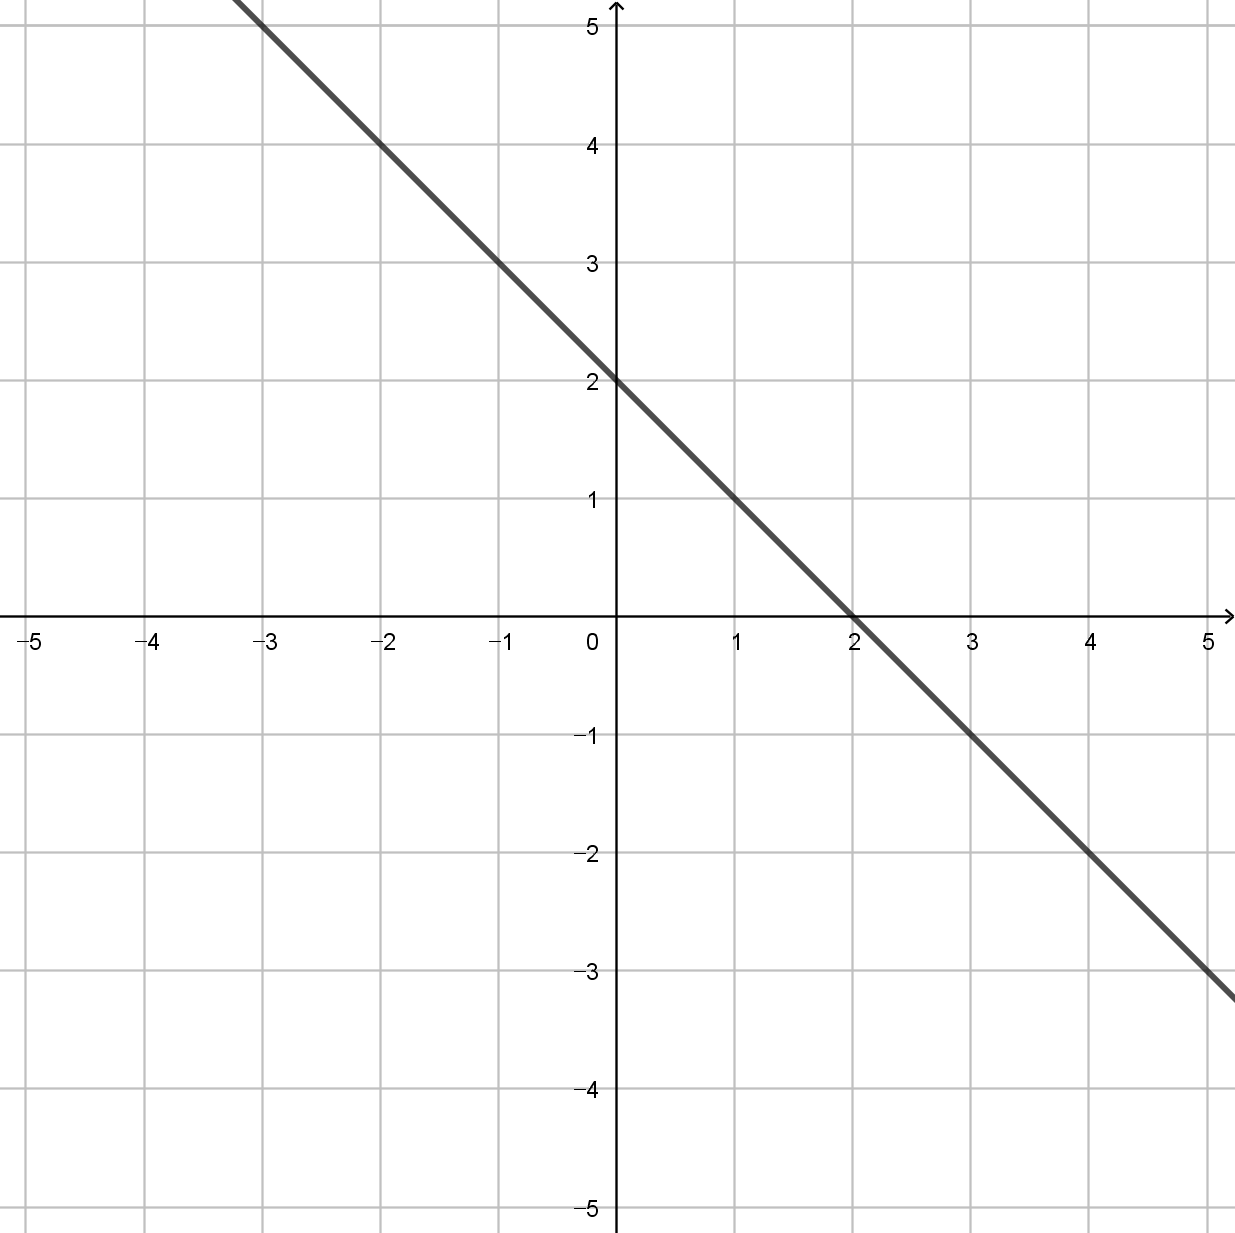
\includegraphics[width=0.9\textwidth]{img/1_line_9}
\end{minipage}
\begin{minipage}{0.45\textwidth}\centering
\(y=2x\)
\par\bigskip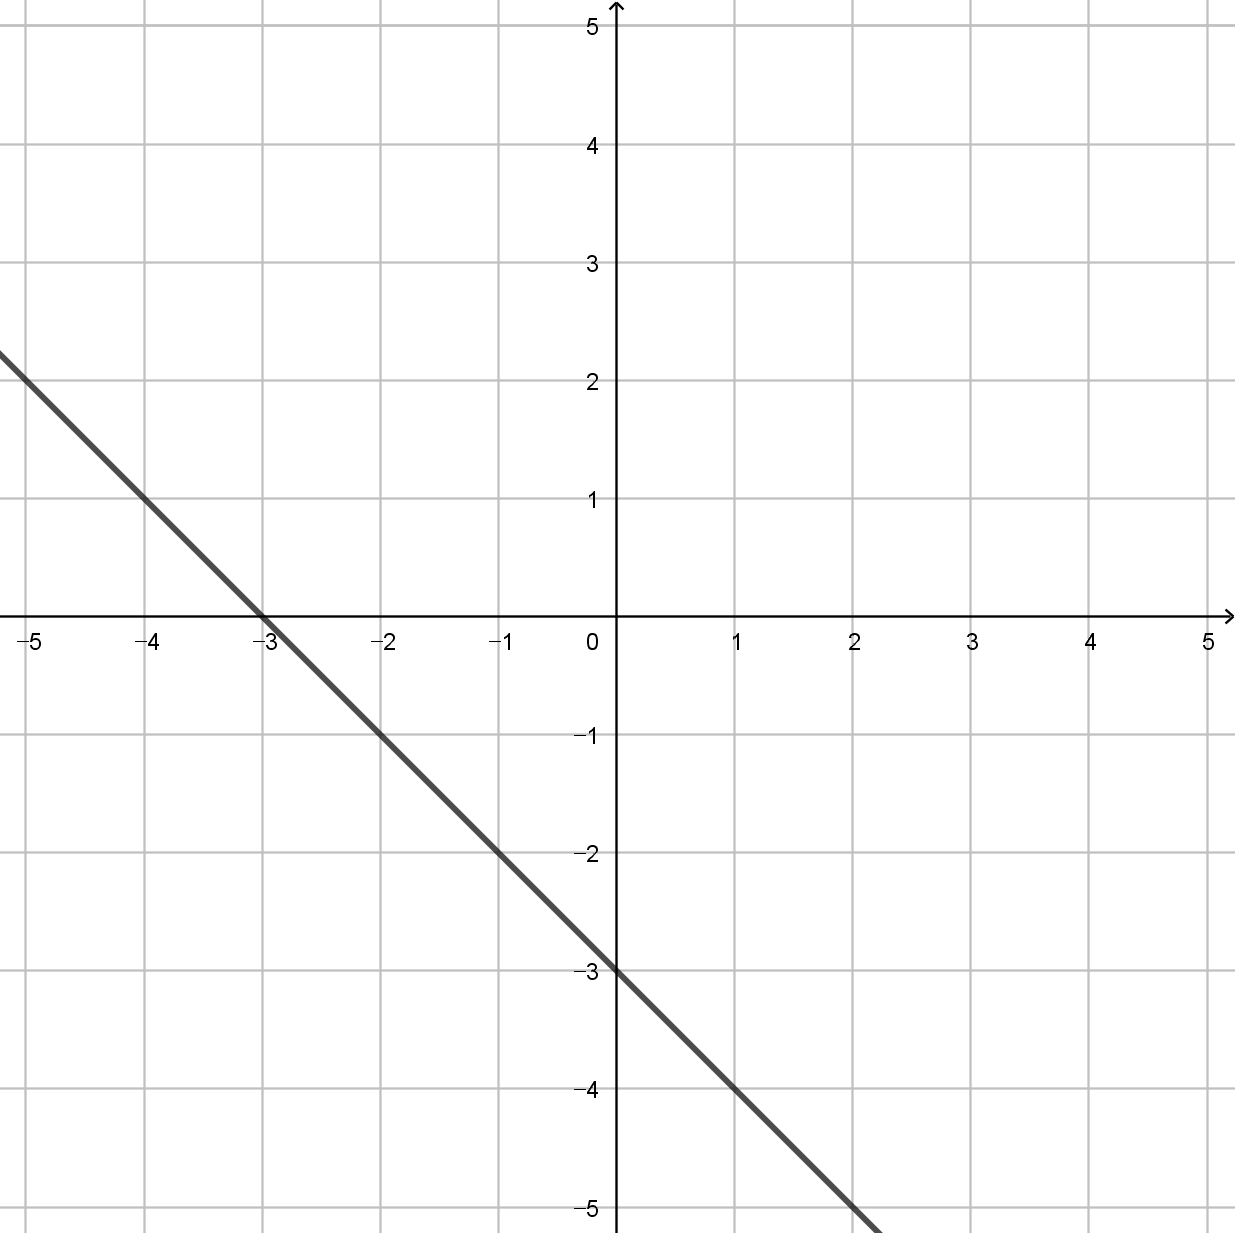
\includegraphics[width=0.9\textwidth]{img/1_line_10}
\end{minipage}\bigskip\bigskip\par

\clearpage
\begin{minipage}{0.45\textwidth}\centering
\(y=3x-3\)
\par\bigskip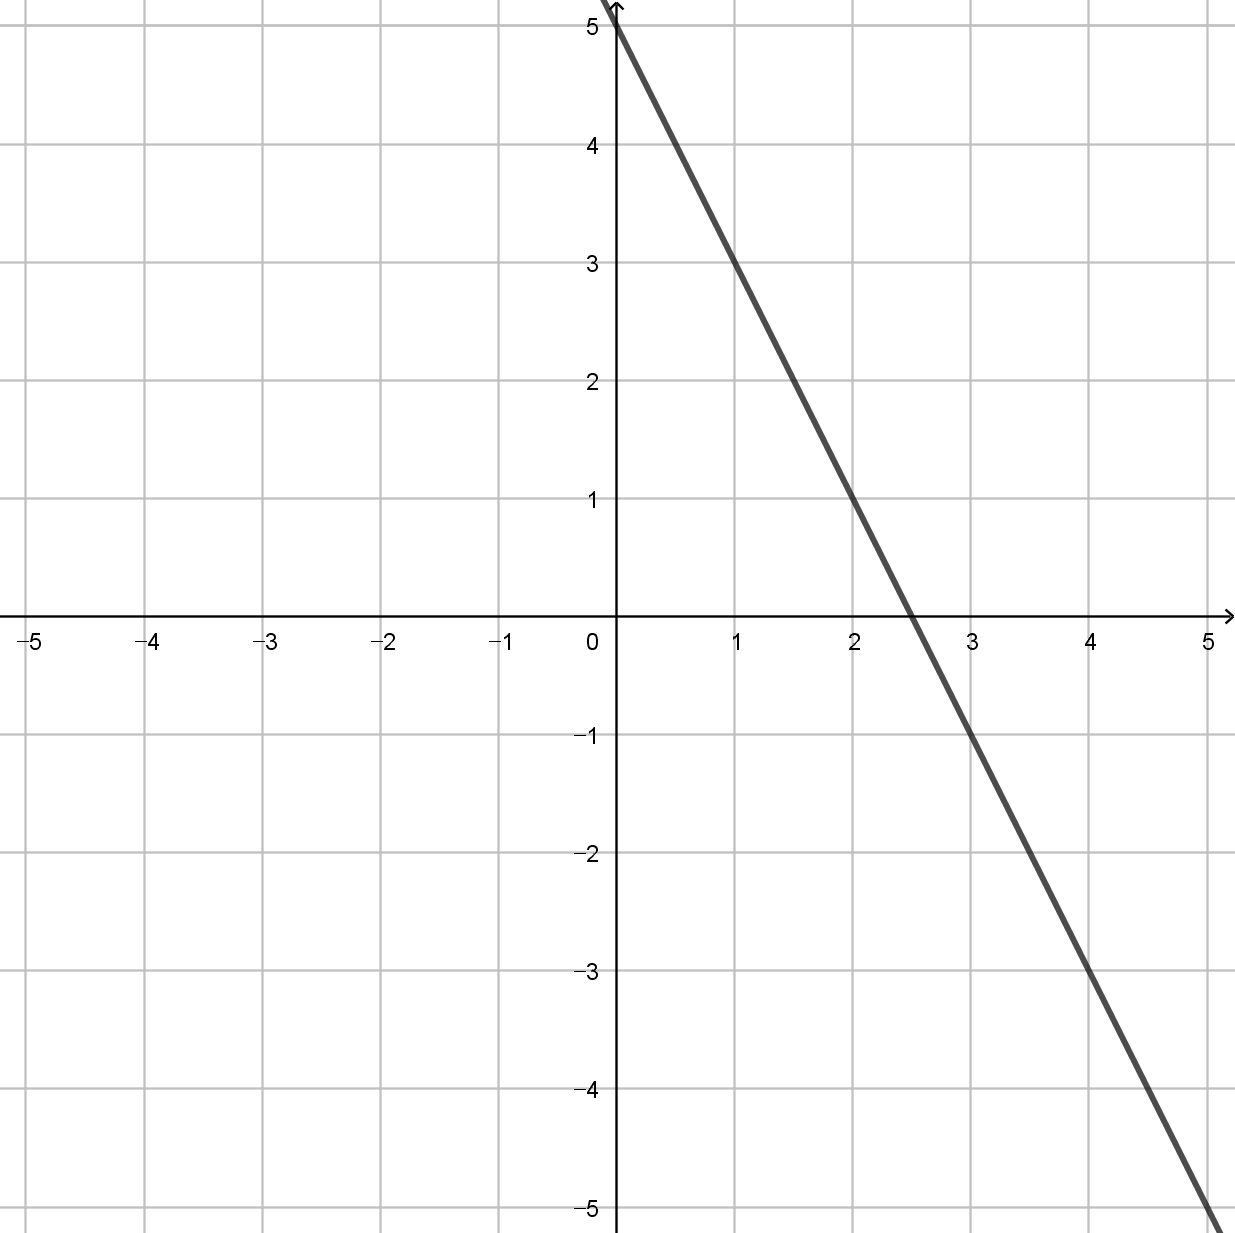
\includegraphics[width=0.9\textwidth]{img/1_line_11}
\end{minipage}
\begin{minipage}{0.45\textwidth}\centering
\(y=3x+2\)
\par\bigskip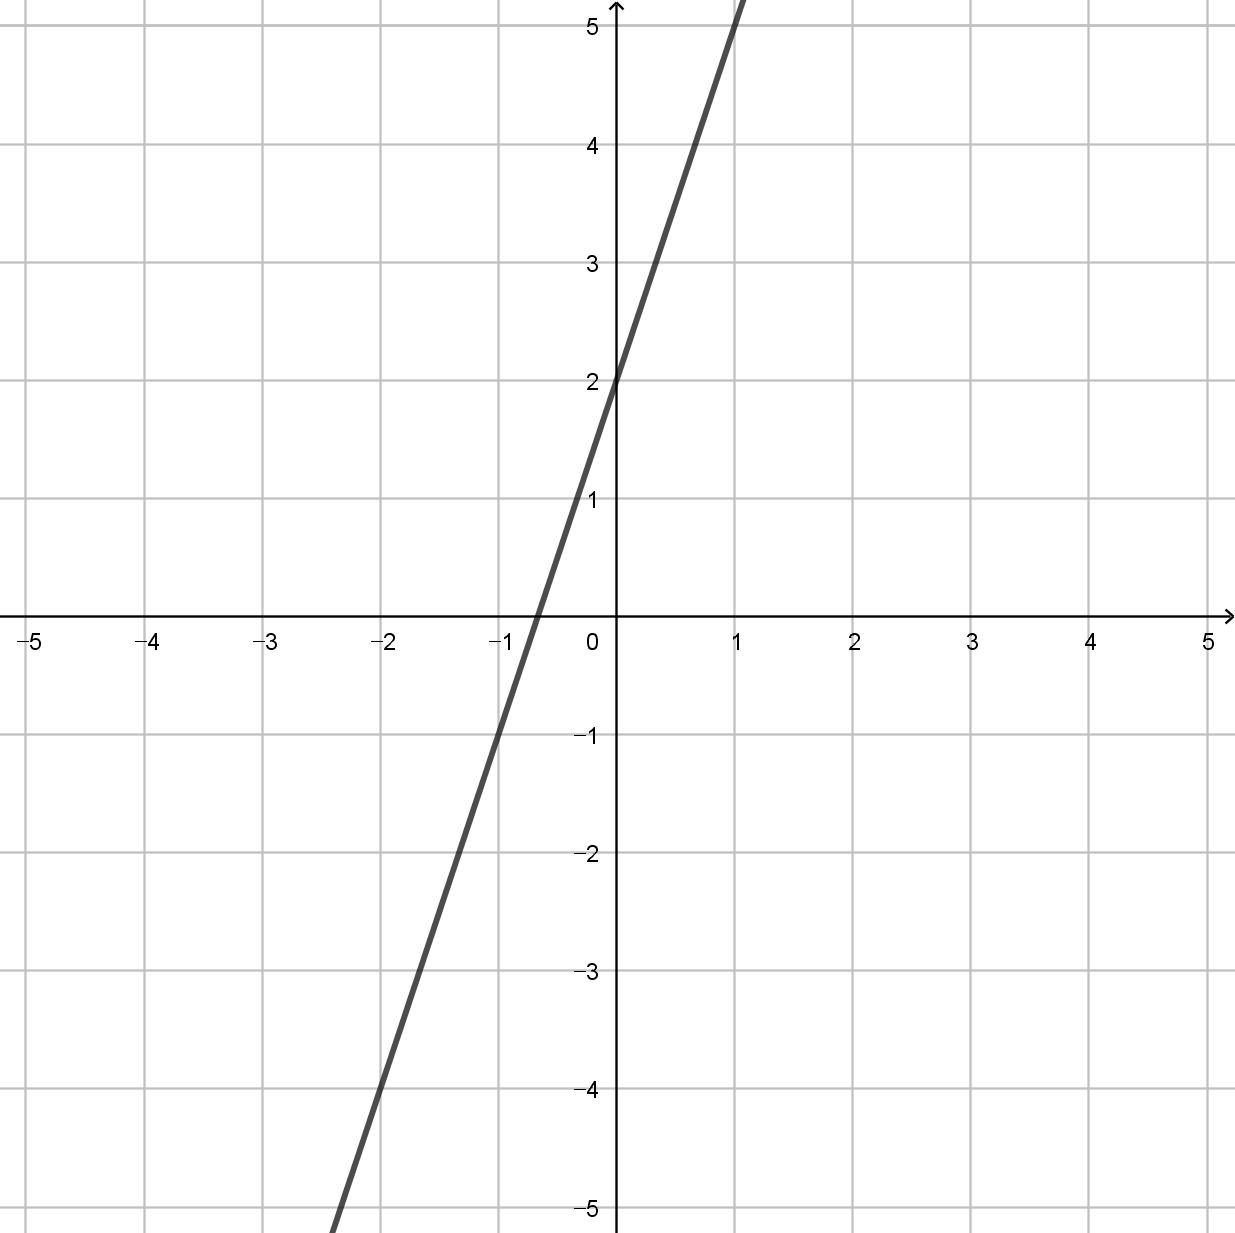
\includegraphics[width=0.9\textwidth]{img/1_line_12}
\end{minipage}\bigskip\bigskip\par
\begin{minipage}{0.45\textwidth}\centering
\(y=-x+2\)
\par\bigskip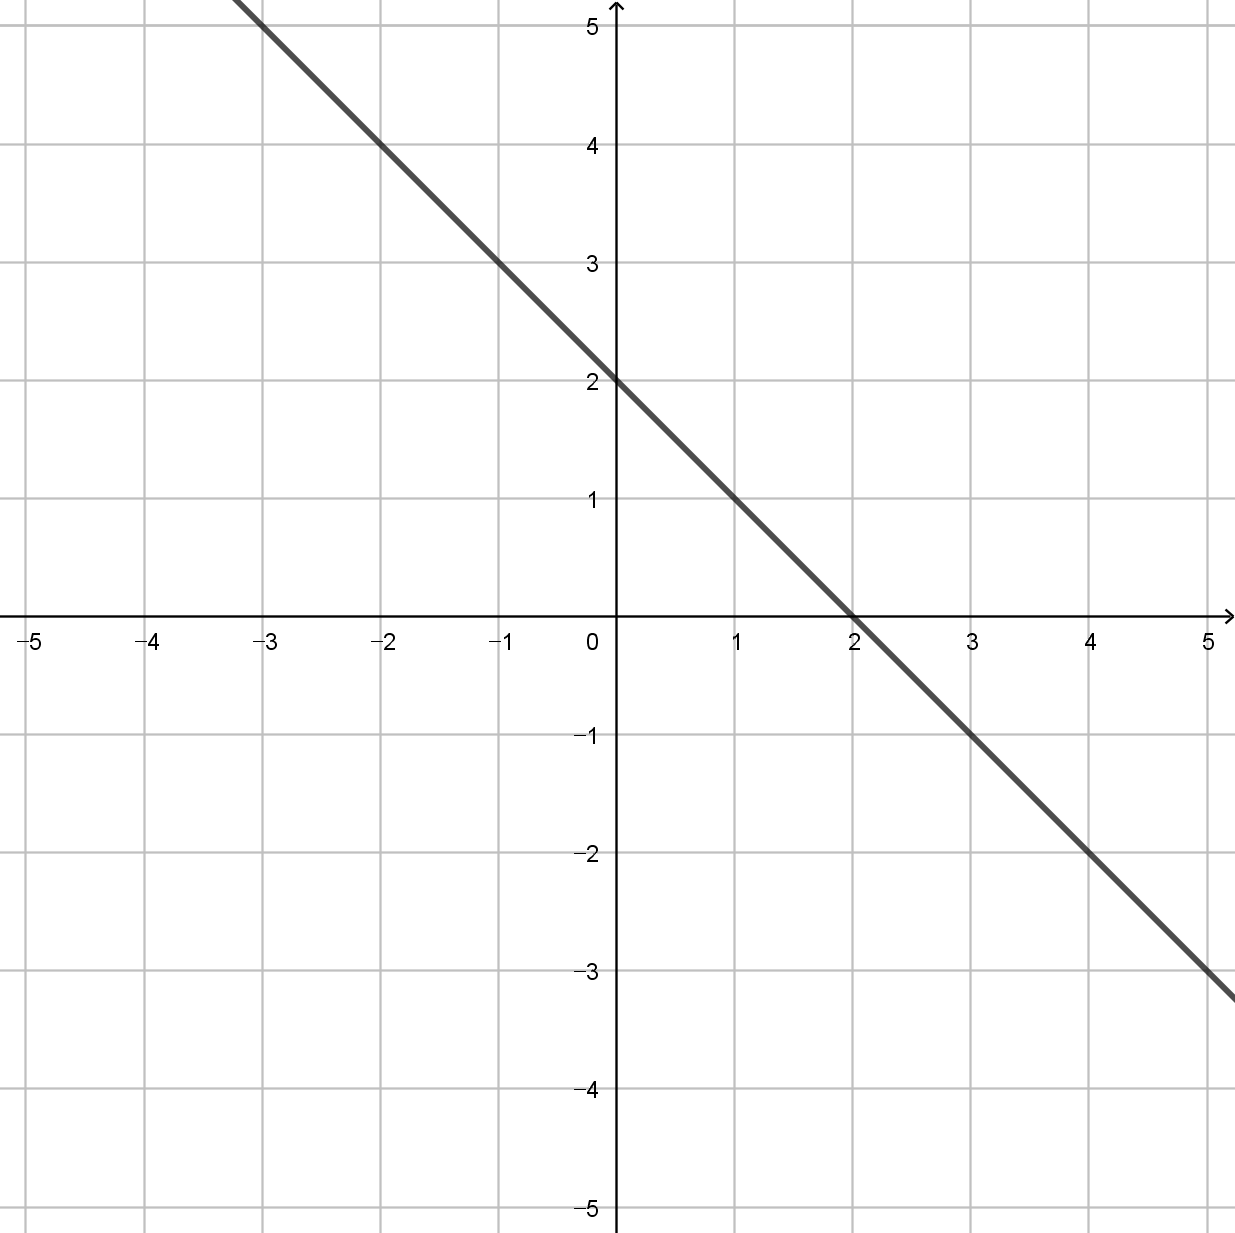
\includegraphics[width=0.9\textwidth]{img/1_line_13}
\end{minipage}
\begin{minipage}{0.45\textwidth}\centering
\(y=-x-3\)
\par\bigskip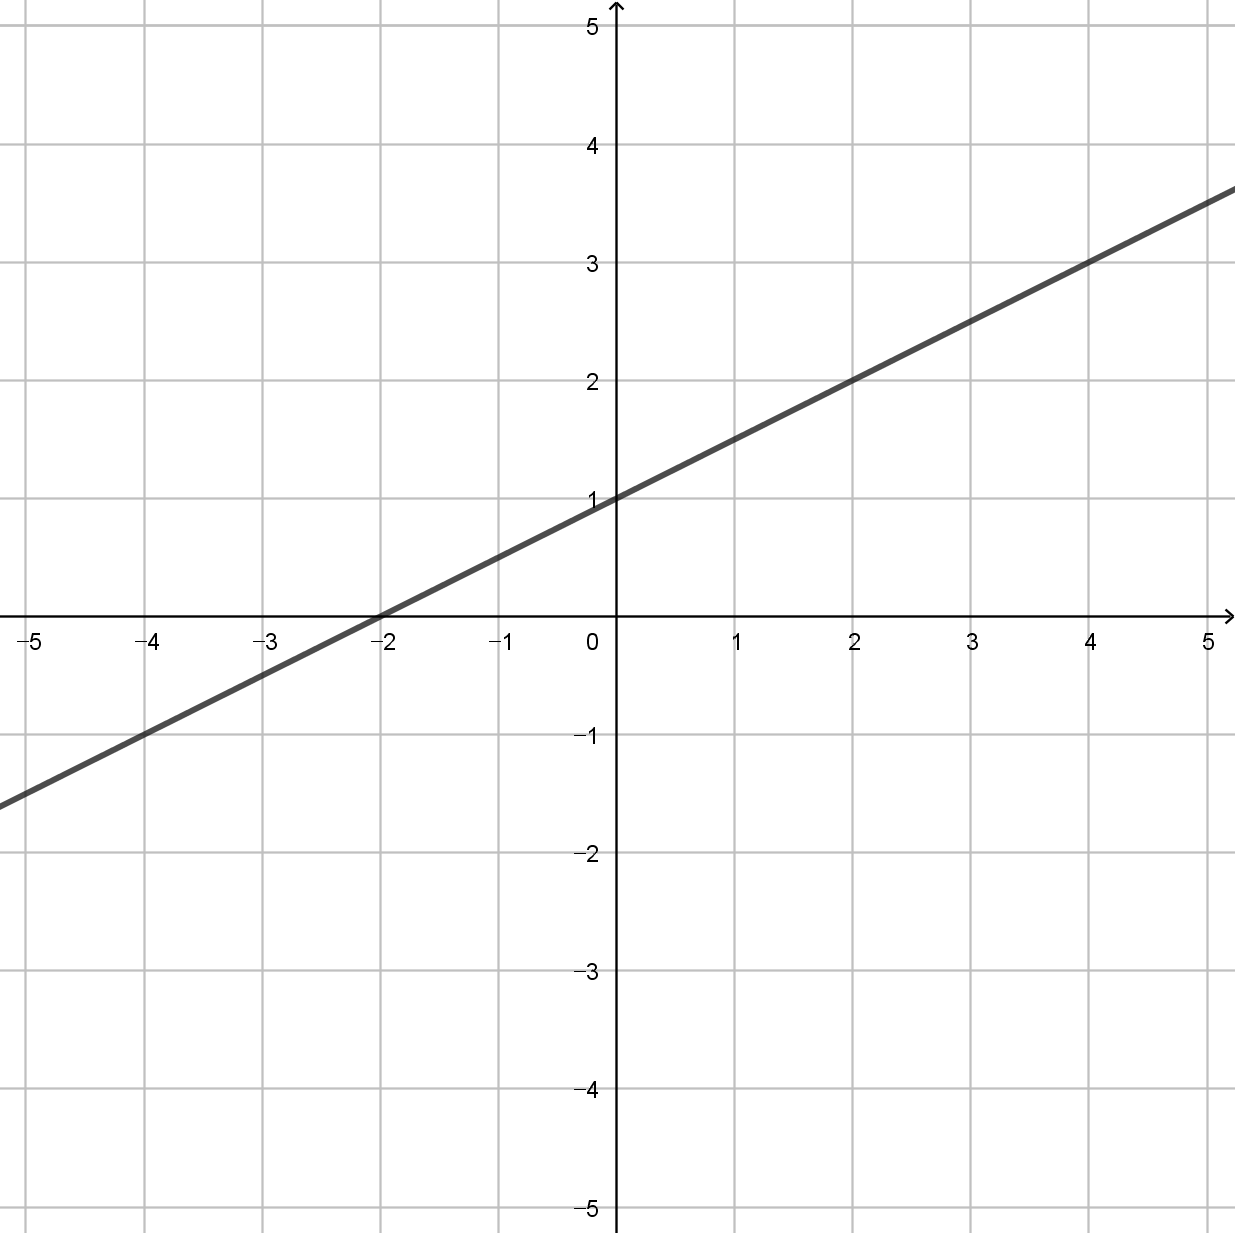
\includegraphics[width=0.9\textwidth]{img/1_line_14}
\end{minipage}\bigskip\bigskip\par
\begin{minipage}{0.45\textwidth}\centering
\(y=-2x+5\)
\par\bigskip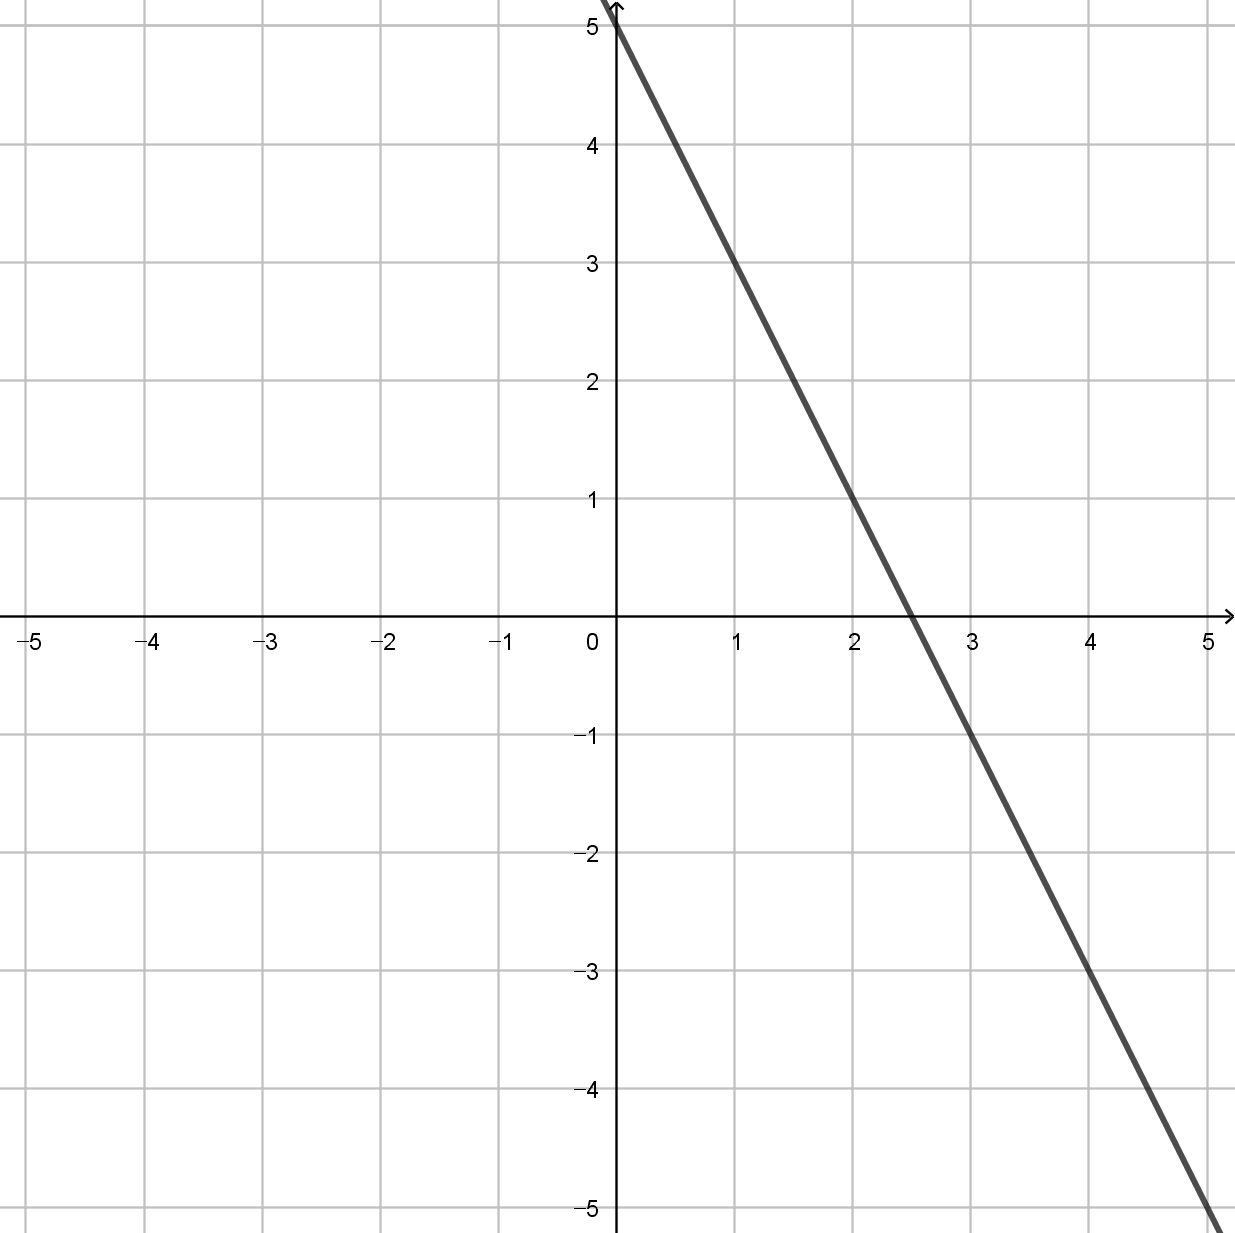
\includegraphics[width=0.9\textwidth]{img/1_line_15}
\end{minipage}
\begin{minipage}{0.45\textwidth}\centering
\(y=-3x+3\)
\par\bigskip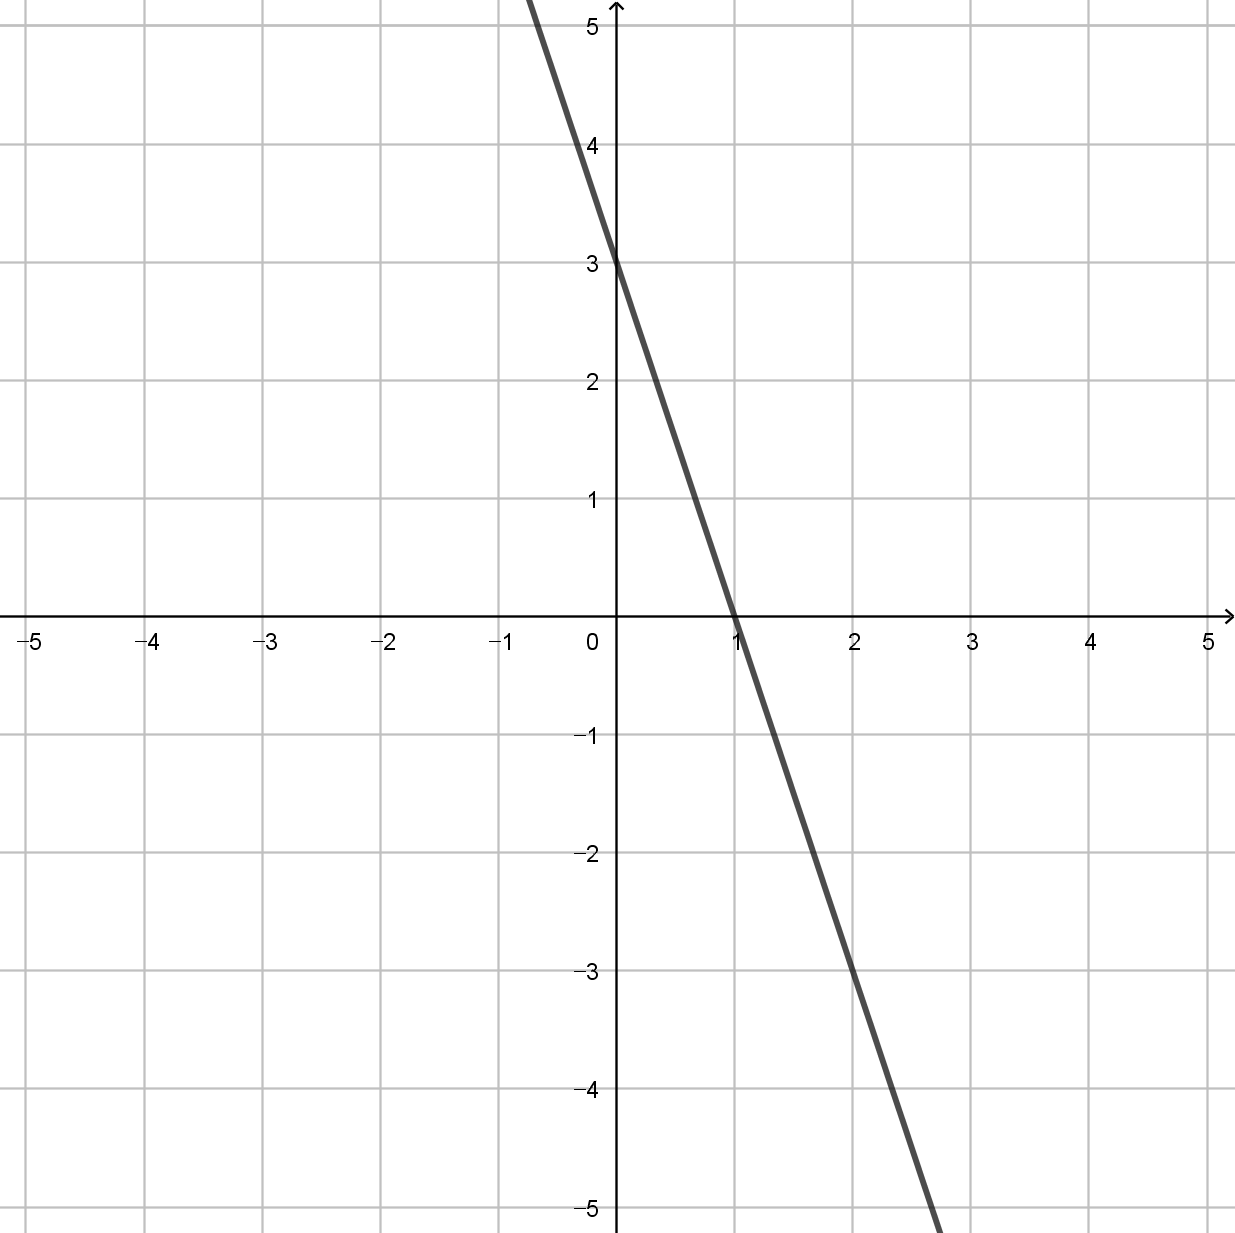
\includegraphics[width=0.9\textwidth]{img/1_line_16}
\end{minipage}\bigskip\bigskip\par


\clearpage
\begin{minipage}{0.45\textwidth}\centering
\(y=\frac12x-2\)
\par\bigskip\includegraphics[width=0.9\textwidth]{img/1_line_17}
\end{minipage}
\begin{minipage}{0.45\textwidth}\centering
\(y=\frac12x+1\)
\par\bigskip\includegraphics[width=0.9\textwidth]{img/1_line_18}
\end{minipage}\bigskip\bigskip\par
\begin{minipage}{0.45\textwidth}\centering
\(y=-\frac12x\)
\par\bigskip\includegraphics[width=0.9\textwidth]{img/1_line_19}
\end{minipage}
\begin{minipage}{0.45\textwidth}\centering
\(y=\frac13x-1\)
\par\bigskip\includegraphics[width=0.9\textwidth]{img/1_line_20}
\end{minipage}\bigskip\bigskip\par
\begin{minipage}{0.45\textwidth}\centering
\(y=\frac23x+2\)
\par\bigskip\includegraphics[width=0.9\textwidth]{img/1_line_21}
\end{minipage}
\begin{minipage}{0.45\textwidth}\centering
\(y=-\frac23x+1\)
\par\bigskip\includegraphics[width=0.9\textwidth]{img/1_line_22}
\end{minipage}\bigskip\bigskip\par


\clearpage
\begin{minipage}{0.45\textwidth}\centering
\(y=\frac32x+3\)
\par\bigskip\includegraphics[width=0.9\textwidth]{img/1_line_23}
\end{minipage}
\begin{minipage}{0.45\textwidth}\centering
\(y=-\frac34x\)
\par\bigskip\includegraphics[width=0.9\textwidth]{img/1_line_24}
\end{minipage}\bigskip\bigskip\par
\begin{minipage}{0.45\textwidth}\centering
\(x+y=1\)
\par\bigskip\includegraphics[width=0.9\textwidth]{img/1_line_25}
\end{minipage}
\begin{minipage}{0.45\textwidth}\centering
\(x+y=-2\)
\par\bigskip\includegraphics[width=0.9\textwidth]{img/1_line_26}
\end{minipage}\bigskip\bigskip\par
\begin{minipage}{0.45\textwidth}\centering
\(2x+y+2=0\)
\par\bigskip\includegraphics[width=0.9\textwidth]{img/1_line_27}
\end{minipage}
\begin{minipage}{0.45\textwidth}\centering
\(3x-2y+6=0\)
\par\bigskip\includegraphics[width=0.9\textwidth]{img/1_line_28}
\end{minipage}\bigskip\bigskip\par


\clearpage
\begin{minipage}{0.45\textwidth}\centering
\(y=3\)
\par\bigskip\includegraphics[width=0.9\textwidth]{img/1_line_29}
\end{minipage}
\begin{minipage}{0.45\textwidth}\centering
\(y=-1\)
\par\bigskip\includegraphics[width=0.9\textwidth]{img/1_line_30}
\end{minipage}\bigskip\bigskip\par
\begin{minipage}{0.45\textwidth}\centering
\(y=0\)
\par\bigskip\includegraphics[width=0.9\textwidth]{img/1_line_31}
\end{minipage}
\begin{minipage}{0.45\textwidth}\centering
\(x=1\)
\par\bigskip\includegraphics[width=0.9\textwidth]{img/1_line_32}
\end{minipage}\bigskip\bigskip\par
\begin{minipage}{0.45\textwidth}\centering
\(x=-2\)
\par\bigskip\includegraphics[width=0.9\textwidth]{img/1_line_33}
\end{minipage}
\begin{minipage}{0.45\textwidth}\centering
\(x=0\)
\par\bigskip\includegraphics[width=0.9\textwidth]{img/1_line_34}
\end{minipage}\bigskip\bigskip\par


\end{document}